% Options for packages loaded elsewhere
\PassOptionsToPackage{unicode}{hyperref}
\PassOptionsToPackage{hyphens}{url}
\documentclass[
  11pt,
]{article}
\usepackage{xcolor}
\usepackage[margin=1in]{geometry}
\usepackage{amsmath,amssymb}
\setcounter{secnumdepth}{-\maxdimen} % remove section numbering
\usepackage{iftex}
\ifPDFTeX
  \usepackage[T1]{fontenc}
  \usepackage[utf8]{inputenc}
  \usepackage{textcomp} % provide euro and other symbols
\else % if luatex or xetex
  \usepackage{unicode-math} % this also loads fontspec
  \defaultfontfeatures{Scale=MatchLowercase}
  \defaultfontfeatures[\rmfamily]{Ligatures=TeX,Scale=1}
\fi
\usepackage{lmodern}
\ifPDFTeX\else
  % xetex/luatex font selection
\fi
% Use upquote if available, for straight quotes in verbatim environments
\IfFileExists{upquote.sty}{\usepackage{upquote}}{}
\IfFileExists{microtype.sty}{% use microtype if available
  \usepackage[]{microtype}
  \UseMicrotypeSet[protrusion]{basicmath} % disable protrusion for tt fonts
}{}
\makeatletter
\@ifundefined{KOMAClassName}{% if non-KOMA class
  \IfFileExists{parskip.sty}{%
    \usepackage{parskip}
  }{% else
    \setlength{\parindent}{0pt}
    \setlength{\parskip}{6pt plus 2pt minus 1pt}}
}{% if KOMA class
  \KOMAoptions{parskip=half}}
\makeatother
\usepackage{longtable,booktabs,array}
\newcounter{none} % for unnumbered tables
\usepackage{calc} % for calculating minipage widths
% Correct order of tables after \paragraph or \subparagraph
\usepackage{etoolbox}
\makeatletter
\patchcmd\longtable{\par}{\if@noskipsec\mbox{}\fi\par}{}{}
\makeatother
% Allow footnotes in longtable head/foot
\IfFileExists{footnotehyper.sty}{\usepackage{footnotehyper}}{\usepackage{footnote}}
\makesavenoteenv{longtable}
\usepackage{graphicx}
\makeatletter
\newsavebox\pandoc@box
\newcommand*\pandocbounded[1]{% scales image to fit in text height/width
  \sbox\pandoc@box{#1}%
  \Gscale@div\@tempa{\textheight}{\dimexpr\ht\pandoc@box+\dp\pandoc@box\relax}%
  \Gscale@div\@tempb{\linewidth}{\wd\pandoc@box}%
  \ifdim\@tempb\p@<\@tempa\p@\let\@tempa\@tempb\fi% select the smaller of both
  \ifdim\@tempa\p@<\p@\scalebox{\@tempa}{\usebox\pandoc@box}%
  \else\usebox{\pandoc@box}%
  \fi%
}
% Set default figure placement to htbp
\def\fps@figure{htbp}
\makeatother
\setlength{\emergencystretch}{3em} % prevent overfull lines
\providecommand{\tightlist}{%
  \setlength{\itemsep}{0pt}\setlength{\parskip}{0pt}}
\usepackage[]{natbib}
\bibliographystyle{plainnat}
\usepackage{bookmark}
\IfFileExists{xurl.sty}{\usepackage{xurl}}{} % add URL line breaks if available
\urlstyle{same}
\hypersetup{
  hidelinks,
  pdfcreator={LaTeX via pandoc}}

\author{}
\date{}

\begin{document}

\section{Compression Favors Consistency, Not Truth: When and Why
Language Models Prefer Correct
Information}\label{compression-favors-consistency-not-truth-when-and-why-language-models-prefer-correct-information}

\textbf{Author:} Konstantin Krestnikov \textbf{Date:} 03.2026

\subsection{Abstract}\label{abstract}

Why do language models sometimes prefer correct statements even when
trained on mixed-quality data? We propose the Compression--Consistency
Principle: gradient descent favors the most compressible hypothesis, not
truth per se. Truth bias emerges only when false alternatives are harder
to compress.

We test this with GPT-2 style character-level transformers (3.5M--86M
parameters) on synthetic corpora mixing correct and incorrect
mathematical derivations. With random errors, models prefer correct
completions 83\% of the time at 50/50 and 67\% even at 10/90. Replacing
random errors with a coherent but wrong rule system eliminates the
effect (accuracy \textasciitilde49\% across all model sizes). The
compression ratio gap between correct and incorrect completions,
measured by gzip on raw text, predicts model behavior across 9
conditions (Spearman rho = 0.68, p = 0.042). A generation sanity check
confirms the direction beyond forced-choice evaluation (30.5\% vs 20.8\%
generative accuracy, p = 0.013).

Two boundary conditions emerge: multi-rule errors produce a graded
increase in truth bias as rule diversity grows, and embedding
verification steps within coherent tasks restores preference for correct
completions (43\% to 71\%). The main implication for alignment:
compression alone does not reliably favor truth over well-structured
falsehood.

\begin{center}\rule{0.5\linewidth}{0.5pt}\end{center}

\subsection{1. Introduction}\label{introduction}

Language models are increasingly accurate on factual benchmarks, yet
they confidently generate false statements. What determines when a model
prefers truth and when it doesn't?

Several explanations have been proposed. Scaling helps: larger models
perform better on factual tasks (Kadavath et al., 2022). RLHF and
similar alignment techniques steer models toward human-preferred
outputs. Data statistics play a role: factual accuracy correlates with
the frequency and source reliability of facts in training data (Elazar
et al., 2022; Joshi et al., 2024; Kandpal et al., 2023). Internal truth
representations have been discovered in model activations (Burns et al.,
2023; Marks \& Tegmark, 2023). Yet none of these explanations address a
more fundamental question: \emph{why would the training objective itself
-- next-token prediction -- create any preference for truth?}

We propose that the answer is compression. Minimizing cross-entropy is
mathematically equivalent to minimizing code length (Shannon, 1948;
Deletang et al., 2024), connecting LLM training to the Minimum
Description Length principle (Rissanen, 1978; Grünwald, 2007). A model
that better predicts tokens is a better compressor. Compression quality
correlates linearly with model capabilities (Huang et al., 2024), and
LLM training formally approximates Solomonoff induction (Wan \& Mei,
2025). But compression does not inherently favor truth -- it favors the
most \emph{compressible} hypothesis consistent with the data. We call
this the \textbf{Compression--Consistency Principle}: truth benefits
from compression only when falsehood is structurally incoherent. Diverse
errors must be memorized individually, whereas a correct rule system
compresses into a compact representation. When errors form a coherent
alternative system -- internally consistent but wrong -- they compress
just as efficiently, and the preference vanishes.

Three caveats apply. First, models compress \emph{text}, not reality:
``truth'' here means correctness of mathematical derivations. Second,
frequency can override compressibility. Third, the compressibility gap
is corpus-dependent, not universal. We test the principle through 9
experiments on mathematical and natural-language synthetic corpora
(Sections 4--7, Appendix B), with models from 3.5M to 86M parameters,
under both character-level and BPE tokenization.

The work makes four contributions. (1) A controlled design in which
\emph{coherent-false} errors serve as a strong null, isolating
compressibility from truth value. (2) Paired evaluation as the primary
metric, revealing that corpus-level loss systematically overestimates
truth bias (Sections 4.1 and 6). (3) Coherent falsehood removes paired
preference across the 3.5M--86M size range, bounding when compression
alone aligns with correctness. (4) Quantitative validation: the
compression ratio gap (measured by gzip on raw text) predicts model
behavior across 9 conditions (Spearman rho = 0.68, p = 0.042), learning
curves confirm behavioral convergence, and a generation sanity check
rules out forced-choice artifacts.

\subsection{2. Related Work}\label{related-work}

\subsubsection{Prediction as
Compression}\label{prediction-as-compression}

The link between prediction and data compression traces back to the
foundational work in information theory. Shannon (1948) showed that
optimal compression requires knowledge of the true data distribution,
and Solomonoff (1964) formalized optimal prediction as weighting
hypotheses by their program length. Rissanen (1978) developed the
Minimum Description Length (MDL) principle, formalizing model selection
as a compression task: the best model minimizes the total description
length of the model plus the data given the model. Grünwald (2007)
systematized the MDL principle and showed its equivalence to several
forms of statistical inference. Hutter (2005) developed these ideas into
a formal theory of universal artificial intelligence (AIXI), explicitly
linking intelligence to compression ability. Our work directly builds on
the MDL framework: we experimentally vary the description length of
false systems and observe under what conditions the MDL-optimal choice
coincides with truth.

In the context of language models, Deletang et al.~(2024) empirically
demonstrated that LLMs are universal compressors: a next-token predictor
can serve as an arithmetic coder. Huang et al.~(2024) discovered a
linear correlation (r \textasciitilde{} -0.95) between compression
quality and benchmark performance, and Wan \& Mei (2025) formally proved
that LLM training approximates Solomonoff induction. Pan et al.~(2025)
used compression-based analysis to explain knowledge acquisition, data
generation, and scaling behaviors. These results form the theoretical
foundation of our work: if LLM training is compression, under what
conditions does compression align with behavior that favors correct over
incorrect continuations?

\subsubsection{Internal Representations of Truth in
LLMs}\label{internal-representations-of-truth-in-llms}

Several studies have found that language models form internal
representations correlated with statement truthfulness. Marks \& Tegmark
(2023) showed a linear geometric structure of truthfulness in activation
space (Geometry of Truth), and Burns et al.~(2023) proposed CCS, a
method for discovering truth directions without supervision. Li et
al.~(2023b) identified a 40\% gap between a model's internal knowledge
and its generation, developing Inference-Time Intervention (ITI).
Ravfogel et al.~(2025) proposed the Truth Co-occurrence Hypothesis -- a
mechanism for the emergence of linear truth representations through
co-occurrence of true statements in the corpus. Azaria \& Mitchell
(2023) showed that internal LLM states can distinguish true from false
outputs, and Bürger et al.~(2024) demonstrated that lie detection
transfers robustly across models and domains. Halawi et al.~(2024)
analyzed how models process false demonstrations, finding that larger
models can ``overthink'' and revert to memorized facts. At the
mechanistic level, Ortu et al.~(2024) traced how factual recall in MLP
layers competes with counterfactual in-context signals processed by
earlier attention heads. Our work complements these representational and
mechanistic analyses at the behavioral level: we study when compression
produces a paired preference for correct over incorrect continuations in
controlled corpora, leaving activation-level analysis for future work.

\subsubsection{Emergent World Models}\label{emergent-world-models}

Language models can form internal world models from pure text
prediction. Li et al.~(2023a) trained a model to predict Othello moves
and found that it learns a full board representation (Othello-GPT).
Gurnee \& Tegmark (2024) discovered linear representations of space and
time in Llama-2 activations. These results show that sequence
compression can give rise to structured internal representations. Our
work does not probe such representations directly; instead, it asks when
compression yields behavioral preference for correct versus incorrect
continuations.

\subsubsection{Truthfulness and Training Data
Statistics}\label{truthfulness-and-training-data-statistics}

Several works investigate the dependence of factual behavior on the
structure of the training corpus. Joshi et al.~(2024) showed that
truthfulness in LLMs is linked to the structure of ``personas''
(sources) in pretraining data: the model learns persona-specific
patterns and prefers statements associated with reliable sources. Elazar
et al.~(2022) demonstrated that factual predictions strongly depend on
the frequency of facts in training data. Kang \& Choi (2023)
investigated how co-occurrence between statements affects factual
recall, and Kandpal et al.~(2023) showed a direct relationship between
the number of supporting documents in the corpus and model answer
accuracy. On a more theoretical side, Kalai \& Vempala (2024) proved
that calibrated language models must hallucinate at a rate tied to the
corpus's monofact rate, establishing a statistical lower bound on
factual errors. Our work differs from this line in emphasis: frequency
clearly matters in our experiments as well, but we \emph{experimentally
vary} the structure of errors (their compressibility) while controlling
frequencies within each condition. This allows us to isolate one factor
beyond frequency and source reliability rather than claiming that data
statistics play no role.

\subsubsection{Simplicity Bias, Noisy Labels, and
Grokking}\label{simplicity-bias-noisy-labels-and-grokking}

The inductive bias of neural networks towards simple functions is a
well-documented phenomenon. Valle-Perez et al.~(2019) showed an
exponential preference for low-complexity functions, and Mingard et
al.~(2021) proved that SGD approximates Bayesian sampling with a
simplicity prior. Goldblum et al.~(2024) connected this to Kolmogorov
complexity, providing a theoretical basis for the link between
compression and generalization. Bhattamishra et al.~(2023) showed that
transformers exhibit a pronounced simplicity bias, preferring
lower-complexity solutions when multiple hypotheses are consistent with
the data. In a related direction, Mészáros et al.~(2024) studied rule
extrapolation in formal languages through a Solomonoff-inspired lens,
showing that models can generalize compositionally to OOD prompts when
the underlying rules are simple enough.

The noisy labels literature directly parallels our setup. Zhang et
al.~(2017) demonstrated that neural networks can memorize completely
random labels, but when structure is present, they generalize through
it. Rolnick et al.~(2017) showed that learning is robust to massive
label noise -- the network learns the ``clean'' pattern even when noise
overwhelmingly predominates. Our result with random errors (truth bias
at 10/90) directly aligns with these observations: random errors play
the role of noise labels, through which the network generalizes to
structured correct solutions.

The phenomenon of grokking -- delayed generalization -- is also related
to compression. Nanda et al.~(2023) showed that networks discover
Fourier transforms for modular arithmetic, and DeMoss et al.~(2024)
described the phase transition from memorization to generalization
through complexity dynamics. Liu et al.~(2023) interpreted grokking as a
compression process: the network transitions from memorization to a
compact representation. Our experiments with coherent errors directly
connect to simplicity bias: a coherent false system is just as
``simple'' as truth, and compression shows no preference for either.

\subsubsection{Our Contribution}\label{our-contribution}

The works above either study internal truth representations in trained
models, establish theoretical links between compression and
intelligence, or analyze the dependence of truthfulness on data
statistics. To our knowledge, direct training experiments with
systematic variation of \emph{error compressibility} remain limited.
This work contributes one such controlled study. Unlike frequency-based
analyses (Elazar et al., 2022; Kandpal et al., 2023; Joshi et al.,
2024), we fix frequency and vary error structure, showing that at 50/50,
truth bias is 83\% for random errors but 49\% for coherent ones. Unlike
representational studies (Burns et al., 2023; Marks \& Tegmark, 2023;
Ravfogel et al., 2025), we train from scratch and identify behavioral
conditions under which paired preference appears or disappears. Unlike
noisy-label work (Zhang et al., 2017; Rolnick et al., 2017), we show
that ``structured noise'' (coherent errors) is not filtered out. Our
results complement the statistical hallucination bound of Kalai \&
Vempala (2024) by identifying a compression-based mechanism: coherent
falsehood remains attractive regardless of rarity.

\subsection{3. Methodology}\label{methodology}

\subsubsection{3.1 Model and Training}\label{model-and-training}

GPT-2 style decoder-only transformer implemented in MLX. Pre-norm
(LayerNorm before attention/MLP), GELU activation, causal mask.

{\def\LTcaptype{none} % do not increment counter
\begin{longtable}[]{@{}lllll@{}}
\toprule\noalign{}
Config & Layers & d\_model & Heads & Parameters \\
\midrule\noalign{}
\endhead
\bottomrule\noalign{}
\endlastfoot
tiny & 4 & 256 & 4 & 3.5M \\
small & 6 & 384 & 6 & 11M \\
medium & 8 & 512 & 8 & 26M \\
large & 12 & 768 & 12 & 86M \\
\end{longtable}
}

Experiments 1--3 use the tiny config; Experiment 4 (Section 7) repeats
the key conditions across all sizes up to large (86M). Optimizer: AdamW
(weight\_decay=0.01), cosine decay with linear warmup (200 steps),
lr=3e-4, seq\_len=256, batch\_size=32, 5000 steps. All experiments are
repeated with 4 random initializations (seeds 42--45).

\textbf{Justification for the number of seeds.} Most conditions are
repeated with 4 random initializations. This is sufficient to show
whether the direction of an effect is stable across runs, but it does
\textbf{not} tightly estimate between-run uncertainty. We therefore use
seed-level summaries as the main unit for training variability, and
report paired-test statistics within each seed as a separate source of
evidence about the behavior of one trained model on many held-out items.
Combined tests across several conditions are reported only as omnibus
support; they are not a substitute for condition-specific replication.

\subsubsection{3.2 Corpus Generation}\label{corpus-generation}

The generator creates mathematical problems of four types: multi-step
arithmetic, factorization, equation solving, and differentiation. Each
problem is formatted as a step-by-step solution in English, verified by
SymPy. The tokenizer is character-level (vocab size = 57) to exclude BPE
artifacts as a confound.

\textbf{Error Types:} - \textbf{Random:} Injection of one plausible
error at a random step (sign, coefficient, distributivity error). Each
error is unique. - \textbf{Coherent:} One systematic incorrect rule per
problem type (e.g., a \ensuremath{\times} b = a \ensuremath{\times} (b\ensuremath{-}1); sign is preserved when moving
terms across =; etc.). All problems of one type fail identically. -
\textbf{Contradictory:} Simple rules (a + b = a + b + 1; a - b = a - b -
2) that break algebraic structure -- addition and subtraction cease to
be inverse operations.

\subsubsection{3.3 Metrics}\label{metrics}

\textbf{Paired evaluation (primary metric).} For each problem, a single
shared prompt is generated along with two completions (correct and
incorrect). NLL is computed only on completion tokens, conditioned on
the shared prompt. This yields pairwise comparison under identical
context, eliminating the confound of different prompts. Metrics:
\textbf{pair accuracy} (fraction of pairs where the model prefers
correct; our primary metric), mean DLoss on completions, one-sided
Wilcoxon signed-rank test. We adopt paired evaluation as the primary
metric because corpus-level measures can be confounded by differences in
text statistics between correct and incorrect corpora (see Sections 4.1
and 6 for concrete examples of such divergence).

As an auxiliary robustness check for the central math conditions, we
also store two additional paired summaries: total NLL over completion
tokens and length-matched mean NLL, which averages only over the shared
minimum completion length in each pair. These variants preserve the main
sign pattern in the key math comparisons (random 50/50, random 10/90,
coherent 50/50), so the reported mean completion-token NLL remains the
primary paired metric.

\textbf{Corpus-level evaluation (secondary diagnostic).} We report two
corpus-level variants. The legacy estimate samples random windows from
the concatenated correct and incorrect token streams; this preserves
continuity with earlier artifacts but is sensitive to local formatting
and stream boundaries. As a robustness check, we also run a
deterministic example-block evaluation that scores every held-out
problem separately without crossing example boundaries. In both cases
\textbf{DLoss = Loss(incorrect) - Loss(correct)}; a positive value
indicates lower loss on correct examples. We treat these corpus-level
measures as diagnostics rather than as the main truth-bias metric.

\textbf{Statistical analysis.} Each configuration is repeated with 4
random initializations (seeds 42--45), except where noted otherwise. For
training variability we report seed-level effect sizes, means across
seeds, and dispersion across seeds. For individual configurations we use
the two-sided binomial test on seed directions as a small-sample
directional check. For paired evaluation, the \textbf{one-sided}
Wilcoxon signed-rank test
(\texttt{alternative=\textquotesingle{}greater\textquotesingle{}}) is
applied to paired NLL differences within a single trained model; this
quantifies uncertainty over held-out pairs, not uncertainty over the
training procedure. 95\% confidence intervals for DLoss are obtained via
bootstrap and should be interpreted at the corresponding level of
aggregation.

\subsubsection{3.4 Theoretical Framework: Description Length and Theory
Types}\label{theoretical-framework-description-length-and-theory-types}

To interpret Experiments 2--3 we use a typology of theories
distinguished by the description length of the corpus ``theory +
observations.'' The key principle: the model optimizes cross-entropy,
which is equivalent to minimizing expected code length (Shannon, 1948).
A theory that allows shorter encoding of the corpus gains an advantage.

\textbf{Type 1: True theory with concrete predictions.} Predictions
match observations. The ``theory + observations'' corpus compresses
maximally: one rule system explains everything.

\textbf{Type 2: False theory with concrete predictions.} Predictions
diverge from observations. The model must encode both the false rules
and the discrepancies. However, if the discrepancies are
\textbf{regular} (e.g., a \ensuremath{\times} b = a \ensuremath{\times} (b\ensuremath{-}1) always understates by a), the
model can learn a correction, and the additional description length is
small.

\textbf{Type 3a: Theory with non-specific predictions.} The theory does
not specify a ``situation -\textgreater{} outcome'' mapping (e.g.,
``result is moderate''). It does not contradict observations but does
not help predict them either -- it does not reduce code length.

\textbf{Type 3b: Theory with ad hoc correction.} Each discrepancy is
explained by a unique exception rule. Description length grows linearly
with the number of observations -- this is anti-compression.

\subsubsection{3.5 MDL Heuristic Framing: When Does Compression Favor
Truth}\label{mdl-heuristic-framing-when-does-compression-favor-truth}

We state a heuristic MDL interpretation (Rissanen, 1978; Grünwald,
2007). Consider a corpus \(D\) consisting of \(N\) problems, fraction
\(\alpha\) solved according to a true theory \(T_1\) and fraction
\((1 - \alpha)\) according to an alternative theory \(T_2\). An
idealized MDL learner would minimize the two-part code
\(L(M) + L(D|M)\), where \(L(M)\) is model description length and
\(L(D|M)\) is data length given the model. The discussion below is
intended as intuition for the experiments, not as a formal theorem about
finite SGD-trained transformers.

\textbf{Heuristic picture.} Let \(K(T_1)\) and \(K(T_2)\) denote
informal description lengths of theories \(T_1\) and \(T_2\). Then:

\begin{enumerate}
\def\labelenumi{\arabic{enumi}.}
\item
  \textbf{\(K(T_2) \gg K(T_1)\) (random errors).} If false completions
  require many idiosyncratic exceptions, the effective description
  length of the false system grows with corpus size. In that regime, an
  MDL-style learner should tend to favor \(T_1\) even when
  \(\alpha < 0.5\), provided the compressibility advantage is large
  enough relative to model capacity and frequency.
\item
  \textbf{\(K(T_2) \approx K(T_1)\) (coherent errors).} If both systems
  are described by compact rules of comparable complexity, frequency
  should dominate. At \(\alpha = 0.5\) an idealized MDL learner has
  little reason to prefer one system over the other.
\item
  \textbf{\(K(T_2) > K(T_1)\), but \(K(T_2) = O(1)\) (multi-rule
  errors).} Multiple alternative rules increase the description length
  of the false system while keeping it structured. The resulting
  preference for \(T_1\) should depend on how unpredictable rule
  selection is relative to the one-rule coherent baseline. This
  prediction requires matched paired evaluation on the same prompt
  distribution.
\end{enumerate}

Experiments 1, 4, and 6 directly test the first two predictions. The
random/coherent contrast is consistent with the MDL framing: truth bias
is large for random errors
(\$\approx\(83% paired accuracy) and near chance for coherent errors (
\)\approx\$49\%). The rebuilt matched multi-rule experiment also fits
the same qualitative picture: increasing rule diversity raises pair
accuracy from 46.6\% at \texttt{N=1} to 88.3\% at \texttt{N=10}.

\begin{figure}
\centering
\pandocbounded{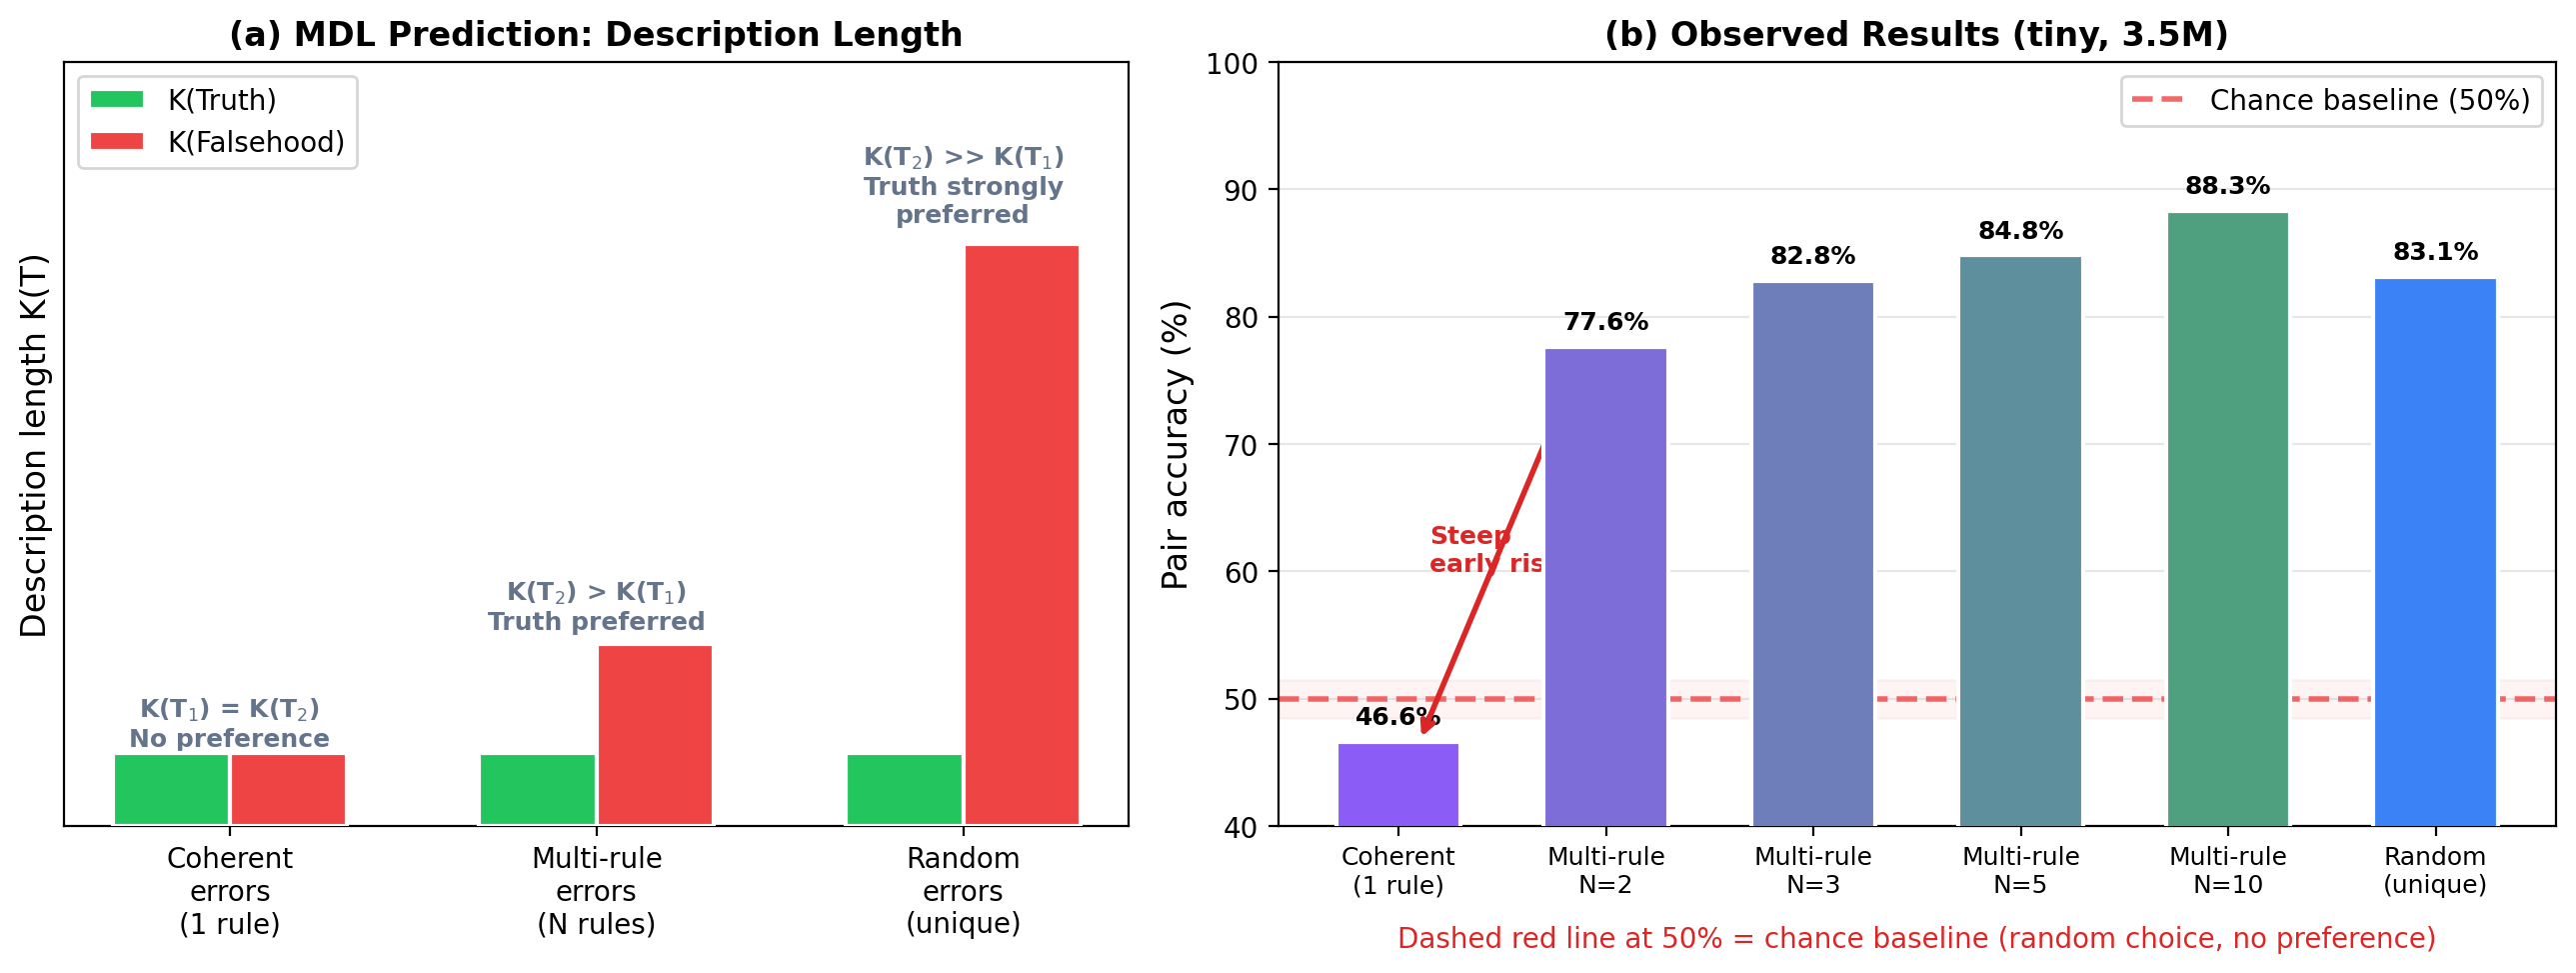
\includegraphics[keepaspectratio,alt={Figure 1}]{figure_conceptual.png}}
\caption{Figure 1}
\end{figure}

\emph{Figure 1. The Compression--Consistency Principle. (a) MDL
prediction: description length of truth \(K(T_1)\) is constant, while
description length of falsehood \(K(T_2)\) depends on error structure --
equal for coherent errors, increasing for multi-rule, maximal for
random. (b) The current experiments support the random/coherent contrast
and show a graded matched multi-rule curve, with the largest increase
between \texttt{N=1} and \texttt{N=2} and continued growth thereafter.}

\textbf{Quantitative compressibility measurement.} To operationalize the
MDL argument, we measure the compression ratio of correct vs.~incorrect
completion segments using gzip (level 9) on concatenated completions
from each paired test set (thousands of completions per condition, to
ensure that compressor header overhead does not dominate). The
compression ratio delta (incorrect minus correct) provides a proxy for
the compressibility gap between correct and incorrect completions,
independent of any trained model.

\textbf{Table C1.} Compression ratio (gzip) of correct vs incorrect
completion segments.

{\def\LTcaptype{none} % do not increment counter
\begin{longtable}[]{@{}lcccc@{}}
\toprule\noalign{}
Condition & Correct & Incorrect & Delta & Paired accuracy \\
\midrule\noalign{}
\endhead
\bottomrule\noalign{}
\endlastfoot
random & 0.1627 & 0.1639 & +0.0012 & 83.1\% \\
coherent & 0.1656 & 0.1658 & +0.0002 & 47.2\% \\
contradictory & 0.1745 & 0.1744 & -0.0001 & 49.0\% \\
multirule N=2 & 0.1671 & 0.1710 & +0.0038 & 77.6\% \\
multirule N=3 & 0.1669 & 0.1722 & +0.0053 & 82.8\% \\
multirule N=5 & 0.1672 & 0.1730 & +0.0057 & 84.8\% \\
multirule N=10 & 0.1676 & 0.1752 & +0.0076 & 88.3\% \\
world random & 0.0370 & 0.0516 & +0.0146 & 57.7\% \\
world coherent & 0.0374 & 0.0384 & +0.0010 & 46.6\% \\
\end{longtable}
}

\begin{figure}
\centering
\pandocbounded{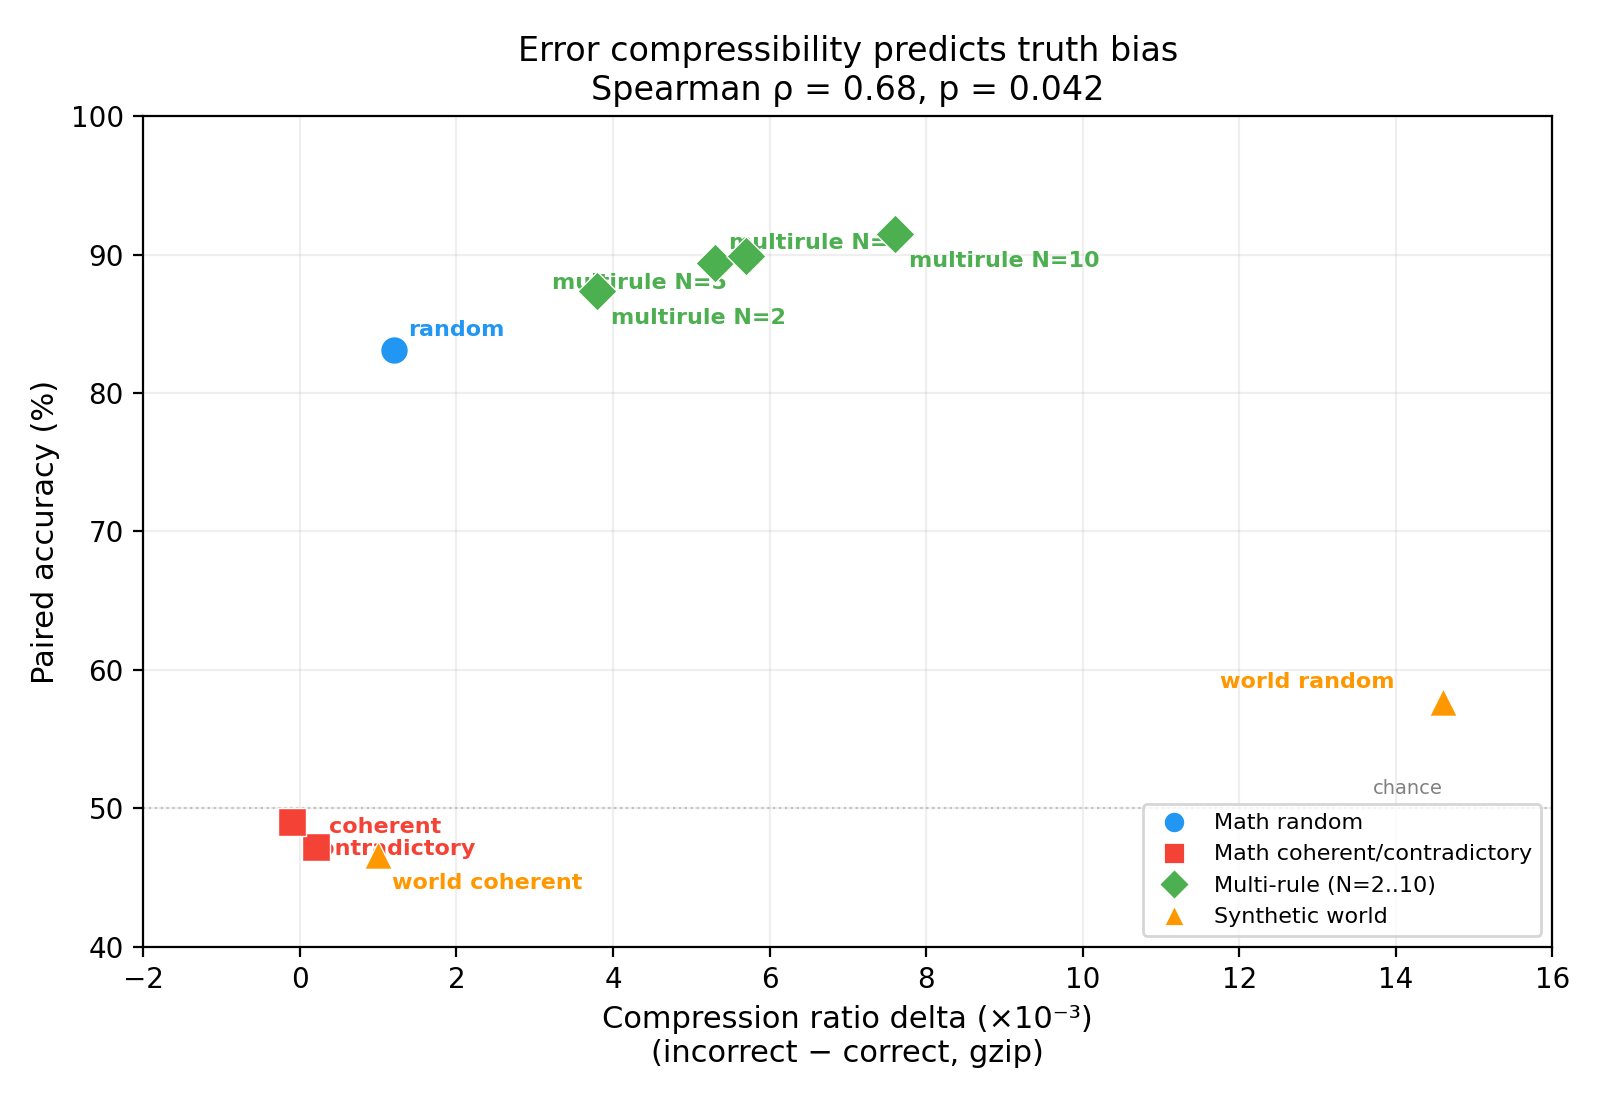
\includegraphics[keepaspectratio,alt={Figure 2}]{figure_compression_vs_accuracy.png}}
\caption{Figure 2}
\end{figure}

\emph{Figure 2. Error compressibility predicts truth bias. Compression
ratio delta (gzip, incorrect minus correct completions) vs paired
accuracy across all conditions. Spearman rho = 0.68, p = 0.042. Coherent
and contradictory errors cluster near zero delta and chance accuracy;
random and multi-rule errors show progressively larger delta and higher
accuracy. The synthetic world domain shows the same qualitative pattern
but at a different scale.}

The rank correlation is significant (Spearman rho = 0.68, p = 0.042),
confirming that the compressibility gap between correct and incorrect
completions -- measurable by a generic compressor without any trained
model -- predicts whether gradient-descent-trained models will exhibit
truth bias. Within the math domain, the multi-rule series shows a
monotonic relationship: N=2 -\textgreater{} N=3 -\textgreater{} N=5
-\textgreater{} N=10 maps to progressively larger compression deltas and
higher paired accuracy. Coherent and contradictory errors have near-zero
delta and near-chance accuracy. The Pearson correlation is lower (r =
0.27, p = 0.49) due to the synthetic world being an outlier -- large
compression delta but modest accuracy, likely because the tiny model
extracts less structure from natural language than from formal math.

\subsubsection{3.6 Experiment Conditions}\label{experiment-conditions}

\textbf{Experiment 1:} 5 proportions (50/50--10/90) x 4 seeds = 20
models with random errors + 1 baseline. Controls: coherent errors (4
proportions x 4 seeds = 16) and contradictory (4 seeds).

\textbf{Experiment 2:} Coherent errors at 50/50 with observations. 4
observation ratios (0\%, 10\%, 25\%, 50\%) x 4 seeds = 16 models. Test
sets contain no observations -- we measure pure mathematical prediction
quality.

\textbf{Experiment 3:} 5 conditions for the false theory (A--E) at
50/50. Conditions A and B are from Experiments 1--2. Conditions C, D, E
-- 3 x 4 seeds = 12 new models.

\textbf{Experiment 4:} Scaling -- random 50/50 is replicated across
small (11M), medium (26M), and large (86M) sizes with 4 seeds per size
in the released artifact set. Coherent 50/50 is now released with 4
seeds at each size from tiny through large. These comparisons are
interpreted as fixed-step trends, not as compute-matched scaling laws.
\textbf{Experiment 5:} Multi-rule errors (matched paired evaluation).
\textbf{Experiment 9:} Chained tasks with verification. Additional
experiments reported in Appendix B: synthetic world, multi-alternative
errors, and cross-domain falsification.

\subsection{4. Experiment 1: Random, Coherent, and Contradictory
Errors}\label{experiment-1-random-coherent-and-contradictory-errors}

\textbf{Hypothesis.} If compression gives rise to truth bias, then
models trained on a mixture of correct and incorrect derivations should
show lower loss on correct examples (DLoss \textgreater{} 0), with the
effect depending on error coherence: random (incoherent) errors
-\textgreater{} strong bias; coherent (systematic) -\textgreater{} weak
or zero.

\subsubsection{4.1 Truth Bias with Random
Errors}\label{truth-bias-with-random-errors}

\textbf{Table 1.} Loss on held-out test sets, averaged over 4 seeds.
DLoss = Loss(incorrect) - Loss(correct); positive value = truth bias.

{\def\LTcaptype{none} % do not increment counter
\begin{longtable}[]{@{}
  >{\raggedright\arraybackslash}p{(\linewidth - 10\tabcolsep) * \real{0.2157}}
  >{\raggedright\arraybackslash}p{(\linewidth - 10\tabcolsep) * \real{0.1569}}
  >{\raggedright\arraybackslash}p{(\linewidth - 10\tabcolsep) * \real{0.1765}}
  >{\raggedright\arraybackslash}p{(\linewidth - 10\tabcolsep) * \real{0.0686}}
  >{\raggedright\arraybackslash}p{(\linewidth - 10\tabcolsep) * \real{0.2059}}
  >{\raggedright\arraybackslash}p{(\linewidth - 10\tabcolsep) * \real{0.1765}}@{}}
\toprule\noalign{}
\begin{minipage}[b]{\linewidth}\raggedright
Proportion (cor/inc)
\end{minipage} & \begin{minipage}[b]{\linewidth}\raggedright
Loss (correct)
\end{minipage} & \begin{minipage}[b]{\linewidth}\raggedright
Loss (incorrect)
\end{minipage} & \begin{minipage}[b]{\linewidth}\raggedright
DLoss
\end{minipage} & \begin{minipage}[b]{\linewidth}\raggedright
95\% CI (bootstrap)
\end{minipage} & \begin{minipage}[b]{\linewidth}\raggedright
Seeds -\textgreater{} correct
\end{minipage} \\
\midrule\noalign{}
\endhead
\bottomrule\noalign{}
\endlastfoot
100/0 (baseline) & 0.1313 & 0.2028 & +0.0715 & -- & 1/1 \\
50/50 & 0.1384 +/- 0.0009 & 0.1499 +/- 0.0008 & +0.0115 +/- 0.0002 &
{[}+0.0113, +0.0116{]} & 4/4 \\
40/60 & 0.1403 +/- 0.0006 & 0.1492 +/- 0.0003 & +0.0089 +/- 0.0003 &
{[}+0.0087, +0.0092{]} & 4/4 \\
30/70 & 0.1422 +/- 0.0009 & 0.1486 +/- 0.0004 & +0.0064 +/- 0.0006 &
{[}+0.0060, +0.0069{]} & 4/4 \\
20/80 & 0.1455 +/- 0.0007 & 0.1487 +/- 0.0006 & +0.0033 +/- 0.0002 &
{[}+0.0031, +0.0034{]} & 4/4 \\
\textbf{10/90} & \textbf{0.1503 +/- 0.0003} & \textbf{0.1487 +/- 0.0001}
& \textbf{-0.0016 +/- 0.0003} & \textbf{{[}-0.0019, -0.0013{]}} &
\textbf{0/4} \\
\end{longtable}
}

\begin{figure}
\centering
\pandocbounded{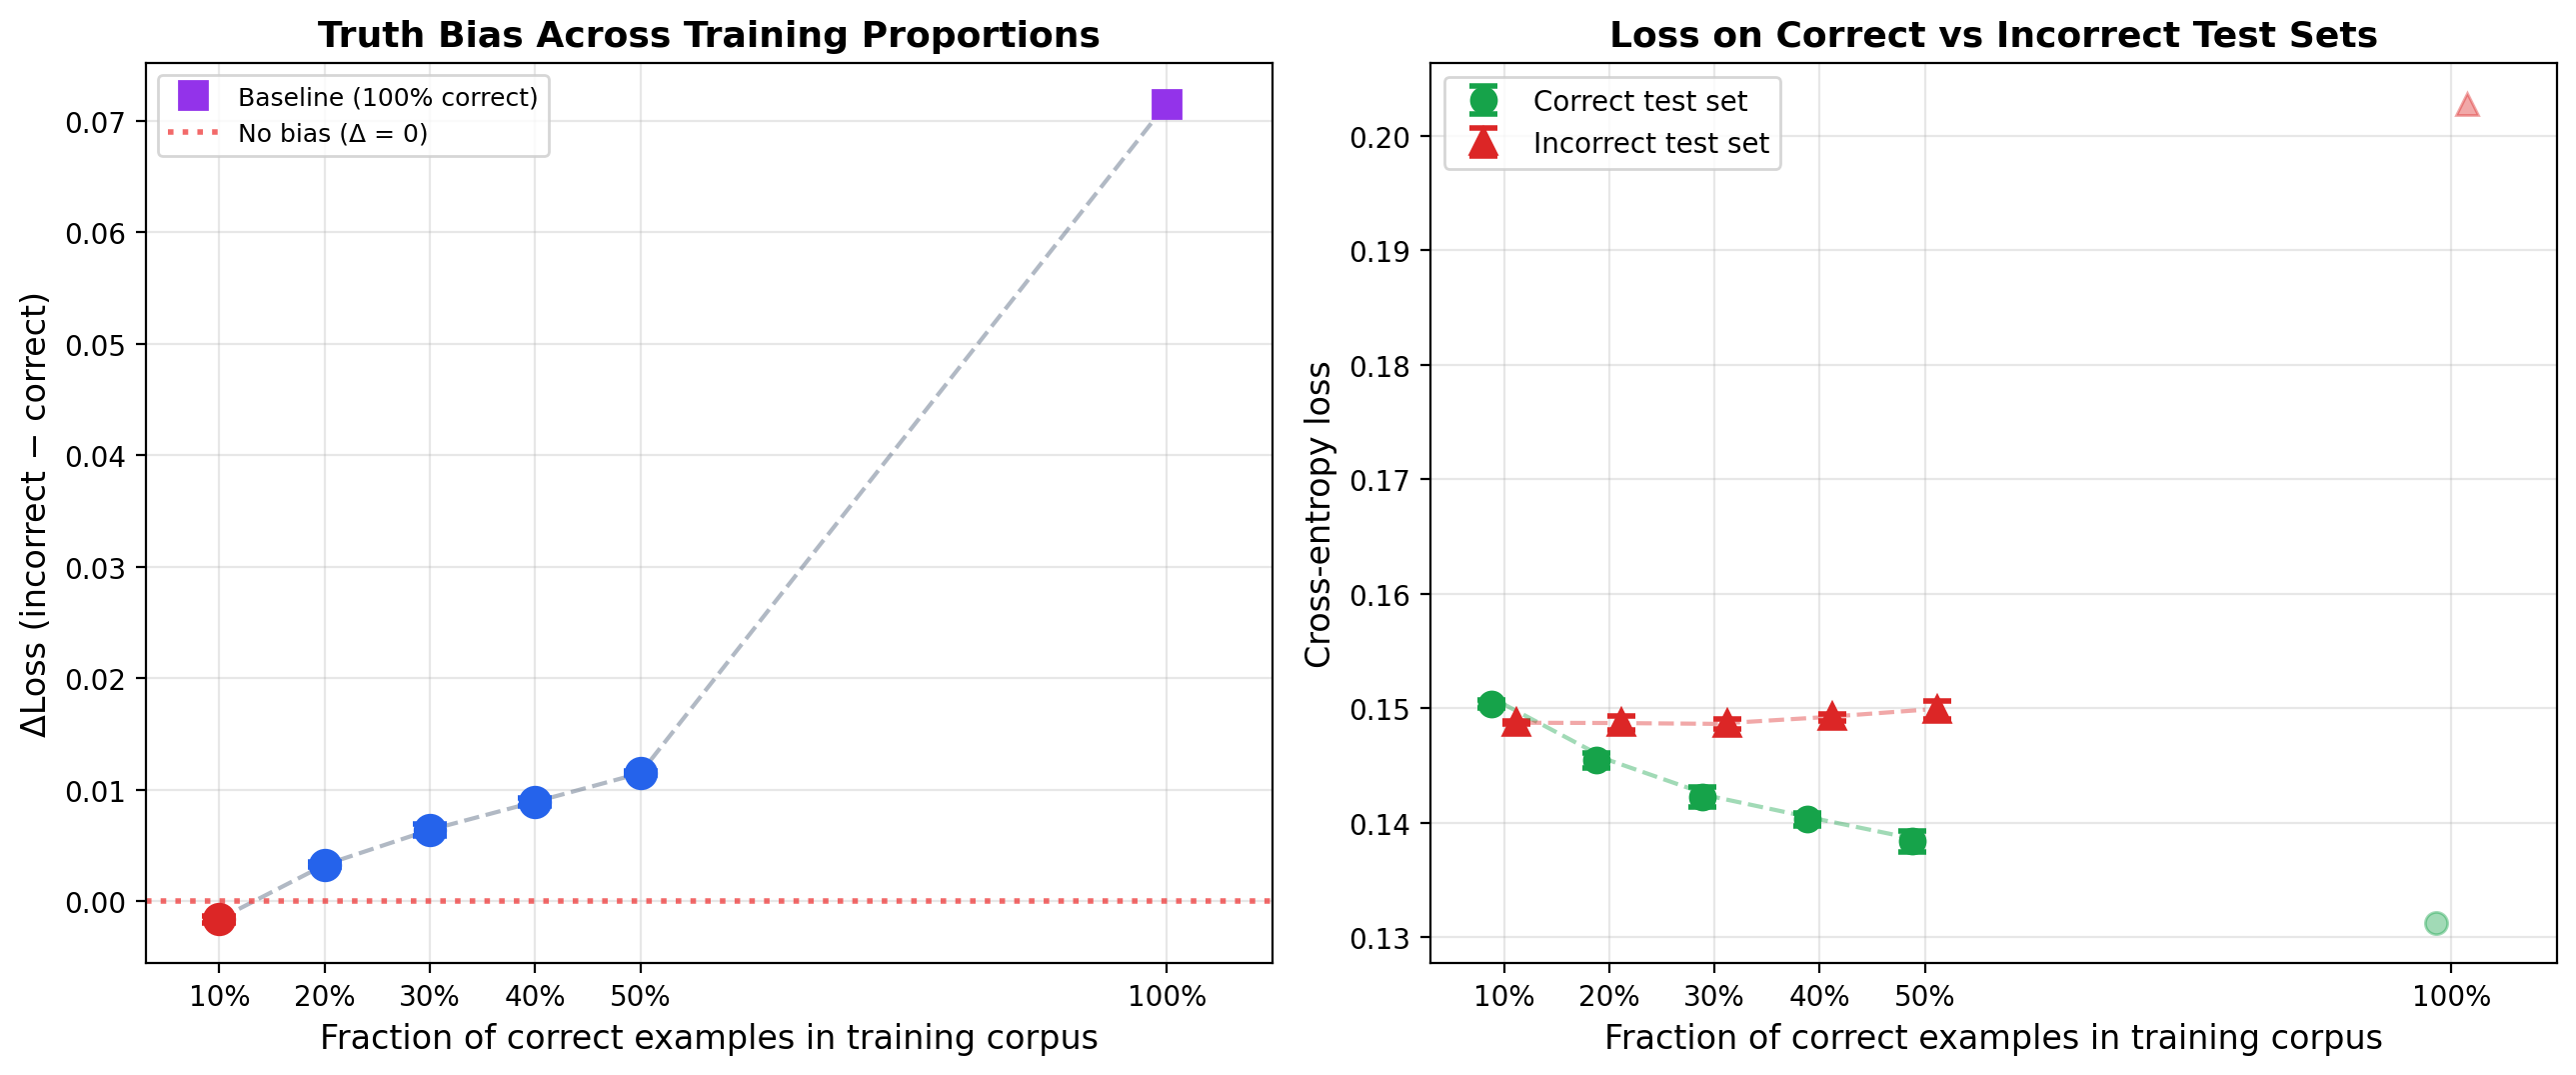
\includegraphics[keepaspectratio,alt={Figure 3}]{figure1_truth_bias.png}}
\caption{Figure 3}
\end{figure}

\emph{Figure 3. Left: DLoss as a function of the correct data fraction.
Truth bias is maintained up to 20/80 and inverts at 10/90 at the corpus
level. Right: absolute loss -- the lines cross at roughly 15\%.}

Corpus-level truth bias decreases strictly monotonically: +0.0115
-\textgreater{} +0.0089 -\textgreater{} +0.0064 -\textgreater{} +0.0033
-\textgreater{} -0.0016. The corpus-level tipping point lies between
10\% and 20\% correct data. Compression pressure beats frequency bias up
to a fourfold prevalence of incorrect data.

An asymmetry is observed: the loss on correct examples increases
substantially (0.1384 -\textgreater{} 0.1503), while the loss on
incorrect ones remains nearly stable (0.1499 -\textgreater{} 0.1487).
The entire dynamic is driven by the model's ability to learn the rules
of correct mathematics.

Statistical significance: 16/16 seeds prefer correct examples at
proportions 50/50--20/80. Two-sided binomial test: p = 3.05 x 10\^{}-5.
For each proportion individually (4/4 seeds) p = 0.125, which is not
significant. The combined test is therefore best viewed as omnibus
support across several related conditions rather than as a substitute
for condition-specific replication.

However, paired evaluation (see below) shows that even at 10/90 the
model retains truth bias at the pair level -- the corpus-level inversion
reflects a frequency effect, not a loss of the structural advantage of
correct solutions.

\textbf{Deterministic full-test robustness check.} The main table above
uses the legacy random-window estimator for continuity with earlier
artifacts, but a deterministic example-block evaluation preserves the
key sign pattern in the central conditions. At random 50/50 it yields
\textbf{DLoss = +0.0157}; at random 10/90 it still yields \textbf{DLoss
= +0.0025} rather than an inversion; and at coherent 50/50 it yields
\textbf{DLoss = -0.0008}. The methodological conclusion is therefore
unchanged: the strongest evidence for truth bias comes from paired
evaluation, while corpus-level estimates are best treated as secondary
diagnostics whose exact magnitude depends on the evaluation procedure.

\textbf{Paired evaluation (50/50, random errors).} To eliminate the
confound of different prompts, we conducted paired evaluation on 4,951
problem pairs with a shared prompt and two completions. This provides a
clearer estimate of the effect:

\textbf{Table 1a.} Paired evaluation at 50/50 (random errors). DLoss =
NLL(incorrect) - NLL(correct) on completion tokens.

{\def\LTcaptype{none} % do not increment counter
\begin{longtable}[]{@{}lcccc@{}}
\toprule\noalign{}
Seed & DLoss (paired) & Pair accuracy & 95\% CI & Wilcoxon p \\
\midrule\noalign{}
\endhead
\bottomrule\noalign{}
\endlastfoot
42 & +0.0478 & 81.5\% & {[}+0.046, +0.050{]} & \textless10\^{}-6 \\
43 & +0.0494 & 84.2\% & {[}+0.047, +0.052{]} & \textless10\^{}-6 \\
44 & +0.0483 & 86.0\% & {[}+0.046, +0.050{]} & \textless10\^{}-6 \\
45 & +0.0465 & 80.8\% & {[}+0.044, +0.049{]} & \textless10\^{}-6 \\
\textbf{Avg} & \textbf{+0.0480} & \textbf{83.1\%} & -- & -- \\
\end{longtable}
}

Given the same prompt, the model assigns lower NLL to the correct
solution 83\% of the time. The effect is \textasciitilde4x larger than
the corpus-level estimate (+0.048 vs +0.012), since the paired metric
isolates the diverging portion of the solution from the shared problem
format.

By problem type, the effect varies: algebra (accuracy 99.9\%)
\textgreater{} arithmetic (94\%) \textgreater{} derivatives (72\%)
\textgreater{} equations (65\%). Algebra shows the cleanest signal: the
model virtually always prefers the correct factorization.

\textbf{Paired evaluation across proportions.} The effect decreases
monotonically but remains significant at all proportions:

\textbf{Table 1b.} Paired evaluation across proportions (random errors,
4 seeds, Wilcoxon p \textless{} 10\^{}-6 for all).

{\def\LTcaptype{none} % do not increment counter
\begin{longtable}[]{@{}cccc@{}}
\toprule\noalign{}
Proportion & Avg DLoss (paired) & Pair accuracy & Corpus DLoss \\
\midrule\noalign{}
\endhead
\bottomrule\noalign{}
\endlastfoot
50/50 & +0.048 & 83\% & +0.0115 \\
40/60 & +0.043 & 79\% & +0.0089 \\
30/70 & +0.036 & 75\% & +0.0064 \\
20/80 & +0.029 & 69\% & +0.0033 \\
\textbf{10/90} & \textbf{+0.017} & \textbf{67\%} & \textbf{-0.0016} \\
\end{longtable}
}

At 10/90, the corpus-level metric inverts (DLoss = -0.0016, the model on
average ``prefers'' incorrect examples due to their 9-fold prevalence),
while paired evaluation consistently shows truth bias (67\% accuracy, p
\textless{} 10\^{}-88). This means that the structural advantage of
correct solutions persists even under extreme imbalance -- the
corpus-level inversion reflects a frequency effect on shared problem
patterns, not a loss of the model's discriminative ability at the level
of individual solutions.

\subsubsection{4.2 Coherent Errors: Disappearance of Truth
Bias}\label{coherent-errors-disappearance-of-truth-bias}

\textbf{Table 2.} Three error types at the 50/50 proportion.

{\def\LTcaptype{none} % do not increment counter
\begin{longtable}[]{@{}
  >{\raggedright\arraybackslash}p{(\linewidth - 10\tabcolsep) * \real{0.1667}}
  >{\raggedright\arraybackslash}p{(\linewidth - 10\tabcolsep) * \real{0.1667}}
  >{\raggedright\arraybackslash}p{(\linewidth - 10\tabcolsep) * \real{0.1667}}
  >{\raggedright\arraybackslash}p{(\linewidth - 10\tabcolsep) * \real{0.1667}}
  >{\raggedright\arraybackslash}p{(\linewidth - 10\tabcolsep) * \real{0.1667}}
  >{\raggedright\arraybackslash}p{(\linewidth - 10\tabcolsep) * \real{0.1667}}@{}}
\toprule\noalign{}
\begin{minipage}[b]{\linewidth}\raggedright
Error Type
\end{minipage} & \begin{minipage}[b]{\linewidth}\raggedright
Loss (correct)
\end{minipage} & \begin{minipage}[b]{\linewidth}\raggedright
Loss (incorrect)
\end{minipage} & \begin{minipage}[b]{\linewidth}\raggedright
DLoss
\end{minipage} & \begin{minipage}[b]{\linewidth}\raggedright
95\% CI
\end{minipage} & \begin{minipage}[b]{\linewidth}\raggedright
Seeds -\textgreater{} correct
\end{minipage} \\
\midrule\noalign{}
\endhead
\bottomrule\noalign{}
\endlastfoot
Random & 0.1384 +/- 0.0009 & 0.1499 +/- 0.0008 & \textbf{+0.0115 +/-
0.0002} & {[}+0.0113, +0.0116{]} & \textbf{4/4} \\
Contradictory & 0.1406 +/- 0.0009 & 0.1411 +/- 0.0008 & \textbf{+0.0005
+/- 0.0001} & {[}+0.0004, +0.0006{]} & \textbf{4/4} \\
Coherent & 0.1374 +/- 0.0005 & 0.1370 +/- 0.0008 & \textbf{-0.0004 +/-
0.0004} & {[}-0.0006, -0.0001{]} & \textbf{0/4} \\
\end{longtable}
}

\begin{figure}
\centering
\pandocbounded{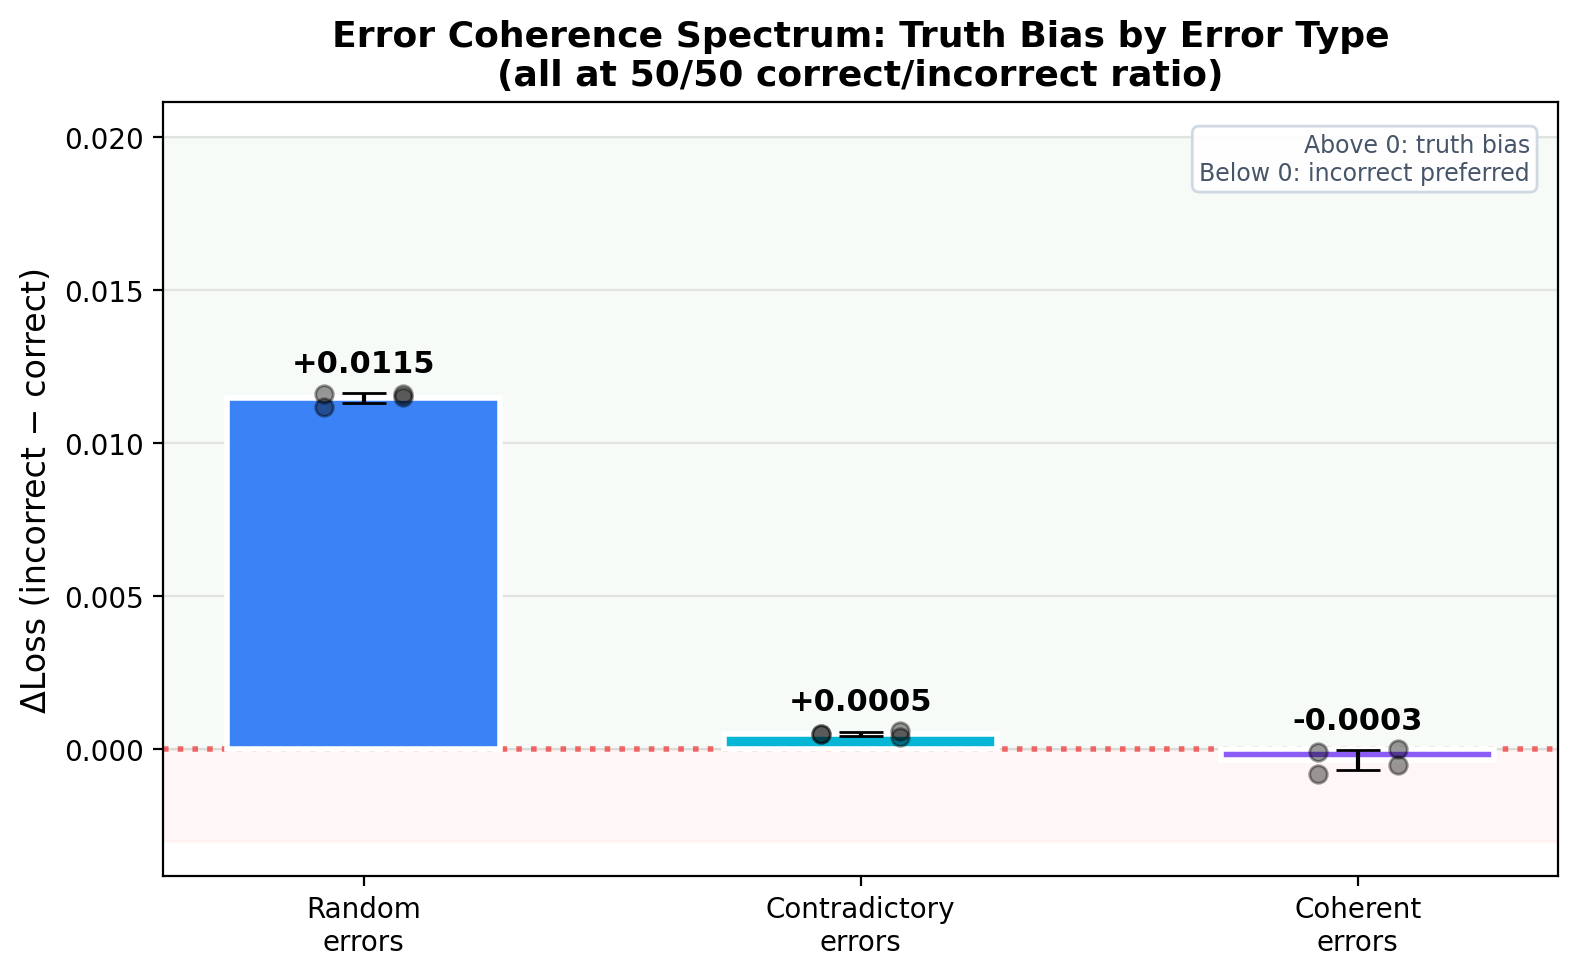
\includegraphics[keepaspectratio,alt={Figure 4}]{figure3_coherence_spectrum.png}}
\caption{Figure 4}
\end{figure}

\emph{Figure 4. Coherence spectrum: DLoss for three error types at
50/50. The less consistent the error system, the stronger the truth
bias.}

The results form a spectrum: random errors (a maximally incoherent
``theory'') yield strong bias; contradictory ones (simple rules that
break algebra) yield a weak one; coherent ones (a consistent system)
yield zero bias.

\textbf{Paired evaluation sharpens the spectrum.} Paired evaluation
(same prompt, two completions) reinforces the picture:

\textbf{Table 2a.} Paired evaluation for three error types at 50/50 (4
seeds).

{\def\LTcaptype{none} % do not increment counter
\begin{longtable}[]{@{}lccc@{}}
\toprule\noalign{}
Error Type & Avg DLoss (paired) & Pair accuracy & Wilcoxon p \\
\midrule\noalign{}
\endhead
\bottomrule\noalign{}
\endlastfoot
Random & \textbf{+0.048} & \textbf{83\%} & \textless10\^{}-6 \\
Contradictory & +0.0003 & 49\% & \textgreater0.3 \\
Coherent & -0.0018 & 47\% & \textasciitilde1.0 \\
\end{longtable}
}

Given the same prompt, the model prefers correct only for random errors.
For coherent and contradictory errors, accuracy remains near chance.
This eliminates the prompt confound and is consistent with the
interpretation that truth bias here depends on error incompressibility
rather than on ``truthfulness'' in the abstract.

\subsubsection{4.3 Coherent Errors at Different
Proportions}\label{coherent-errors-at-different-proportions}

\textbf{Table 3.} Random vs.~coherent errors across proportions.

{\def\LTcaptype{none} % do not increment counter
\begin{longtable}[]{@{}
  >{\raggedright\arraybackslash}p{(\linewidth - 8\tabcolsep) * \real{0.2000}}
  >{\raggedright\arraybackslash}p{(\linewidth - 8\tabcolsep) * \real{0.2000}}
  >{\raggedright\arraybackslash}p{(\linewidth - 8\tabcolsep) * \real{0.2000}}
  >{\raggedright\arraybackslash}p{(\linewidth - 8\tabcolsep) * \real{0.2000}}
  >{\raggedright\arraybackslash}p{(\linewidth - 8\tabcolsep) * \real{0.2000}}@{}}
\toprule\noalign{}
\begin{minipage}[b]{\linewidth}\raggedright
Proportion
\end{minipage} & \begin{minipage}[b]{\linewidth}\raggedright
Random DLoss
\end{minipage} & \begin{minipage}[b]{\linewidth}\raggedright
Coherent DLoss
\end{minipage} & \begin{minipage}[b]{\linewidth}\raggedright
Random -\textgreater{}
\end{minipage} & \begin{minipage}[b]{\linewidth}\raggedright
Coherent -\textgreater{}
\end{minipage} \\
\midrule\noalign{}
\endhead
\bottomrule\noalign{}
\endlastfoot
50/50 & +0.0115 +/- 0.0002 & -0.0004 +/- 0.0004 & correct (4/4) &
incorrect (0/4) \\
40/60 & +0.0089 +/- 0.0003 & -0.0041 +/- 0.0002 & correct (4/4) &
incorrect (0/4) \\
30/70 & +0.0064 +/- 0.0006 & -0.0083 +/- 0.0003 & correct (4/4) &
incorrect (0/4) \\
20/80 & +0.0033 +/- 0.0002 & -0.0143 +/- 0.0006 & correct (4/4) &
incorrect (0/4) \\
\end{longtable}
}

With random errors, truth bias withstands frequency up to 20/80. With
coherent errors, DLoss is negative at all proportions: the model
slightly prefers the incorrect system even at 50/50, and this preference
strengthens as the share of incorrect data grows. The model follows pure
frequency -- preferring whichever type is more abundant (or easier to
compress at equal proportions). \textbf{Truth bias with random errors is
a consequence of the incompressibility of ad hoc errors, not an
intrinsic property of data ``truthfulness.''}

\textbf{Paired evaluation sharpens the contrast.} For coherent errors,
paired evaluation reveals a symmetric picture: the model prefers
whichever system is in the majority.

\textbf{Table 3a.} Paired evaluation for coherent errors across
proportions (4 seeds).

{\def\LTcaptype{none} % do not increment counter
\begin{longtable}[]{@{}
  >{\centering\arraybackslash}p{(\linewidth - 6\tabcolsep) * \real{0.1642}}
  >{\centering\arraybackslash}p{(\linewidth - 6\tabcolsep) * \real{0.2239}}
  >{\centering\arraybackslash}p{(\linewidth - 6\tabcolsep) * \real{0.2836}}
  >{\centering\arraybackslash}p{(\linewidth - 6\tabcolsep) * \real{0.3284}}@{}}
\toprule\noalign{}
\begin{minipage}[b]{\linewidth}\centering
Proportion
\end{minipage} & \begin{minipage}[b]{\linewidth}\centering
Random accuracy
\end{minipage} & \begin{minipage}[b]{\linewidth}\centering
Coherent accuracy
\end{minipage} & \begin{minipage}[b]{\linewidth}\centering
Coherent DLoss (paired)
\end{minipage} \\
\midrule\noalign{}
\endhead
\bottomrule\noalign{}
\endlastfoot
50/50 & 83\% & 47.2\% & -0.002 \\
40/60 & 79\% & 27.8\% & -0.009 \\
30/70 & 75\% & 14.7\% & -0.019 \\
20/80 & 69\% & 9.6\% & -0.033 \\
\end{longtable}
}

The contrast is striking: at 20/80, the model with random errors still
prefers truth (69\%), whereas the model with coherent errors actively
prefers the false system (accuracy 9.6\%, i.e.~in 91\% of pairs the
model assigns lower NLL to the coherent-incorrect solution). Truth has
no privilege -- when compressibility is equal, frequency wins.

\begin{figure}
\centering
\pandocbounded{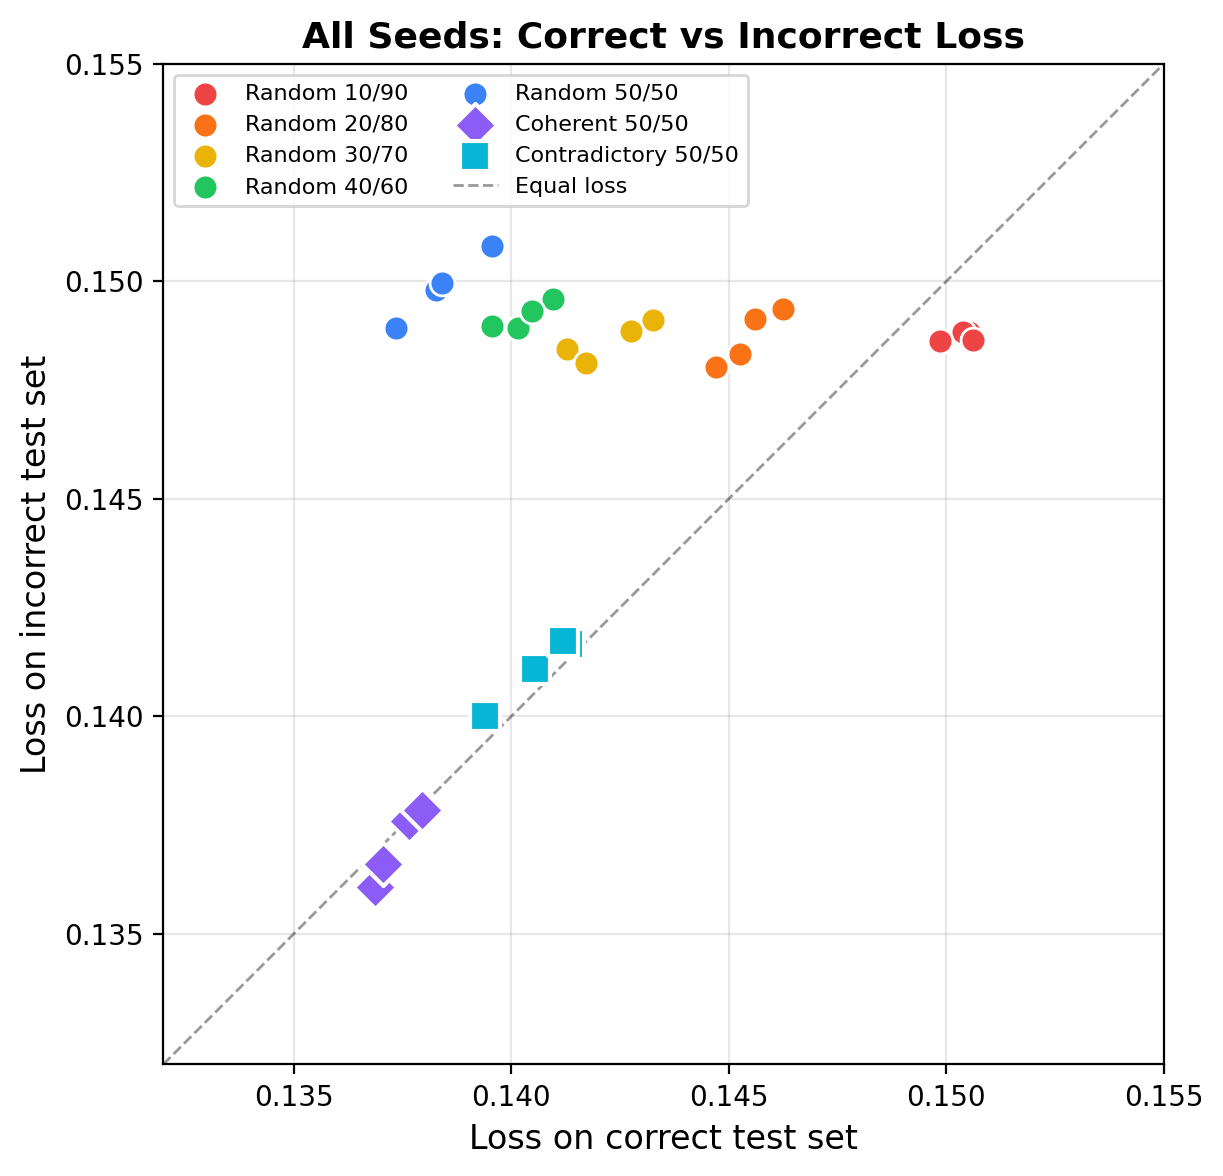
\includegraphics[keepaspectratio,alt={Figure 5}]{figure2_scatter.png}}
\caption{Figure 5}
\end{figure}

\emph{Figure 5. Loss across seeds: points above the diagonal indicate
truth bias. Coherent errors (diamonds) lie on the diagonal.}

\subsection{5. Experiment 2: Observations and Predictive
Power}\label{experiment-2-observations-and-predictive-power}

\textbf{Hypothesis.} Adding empirical feedback (observations) should
increase the description length of the false theory by introducing
discrepancies, thereby restoring truth bias for coherent errors.

Experiment 1 showed that a coherent false system compresses just as well
as the correct one. But in the real world, false theories diverge from
observations. We add a verification component:

\begin{verbatim}
# Correct theory: a x b = a*b
Prediction: total = 50
Observation: counted 50 items [check]

# Coherent false: a x b = a*(b-1)
Prediction: total = 40
Observation: counted 50 items [cross]
\end{verbatim}

\textbf{Table 4.} Impact of observation ratio on truth bias (coherent
errors, 50/50).

{\def\LTcaptype{none} % do not increment counter
\begin{longtable}[]{@{}
  >{\centering\arraybackslash}p{(\linewidth - 10\tabcolsep) * \real{0.1667}}
  >{\centering\arraybackslash}p{(\linewidth - 10\tabcolsep) * \real{0.1667}}
  >{\centering\arraybackslash}p{(\linewidth - 10\tabcolsep) * \real{0.1667}}
  >{\centering\arraybackslash}p{(\linewidth - 10\tabcolsep) * \real{0.1667}}
  >{\centering\arraybackslash}p{(\linewidth - 10\tabcolsep) * \real{0.1667}}
  >{\centering\arraybackslash}p{(\linewidth - 10\tabcolsep) * \real{0.1667}}@{}}
\toprule\noalign{}
\begin{minipage}[b]{\linewidth}\centering
Observation \%
\end{minipage} & \begin{minipage}[b]{\linewidth}\centering
Avg DLoss
\end{minipage} & \begin{minipage}[b]{\linewidth}\centering
95\% CI
\end{minipage} & \begin{minipage}[b]{\linewidth}\centering
Seeds -\textgreater{} correct
\end{minipage} & \begin{minipage}[b]{\linewidth}\centering
p (binom)
\end{minipage} & \begin{minipage}[b]{\linewidth}\centering
Avg Loss (correct)
\end{minipage} \\
\midrule\noalign{}
\endhead
\bottomrule\noalign{}
\endlastfoot
0\% (control)* & +0.0005 +/- 0.0003 & {[}+0.0002, +0.0007{]} & 4/4 &
0.125 & 0.1414 \\
10\% & +0.0002 +/- 0.0003 & {[}-0.0001, +0.0004{]} & 3/4 & 0.625 &
0.1416 \\
25\% & +0.0004 +/- 0.0001 & {[}+0.0003, +0.0004{]} & 4/4 & 0.125 &
0.1435 \\
50\% & +0.0008 +/- 0.0006 & {[}+0.0003, +0.0012{]} & 3/4 & 0.625 &
0.1471 \\
\end{longtable}
}

\begin{figure}
\centering
\pandocbounded{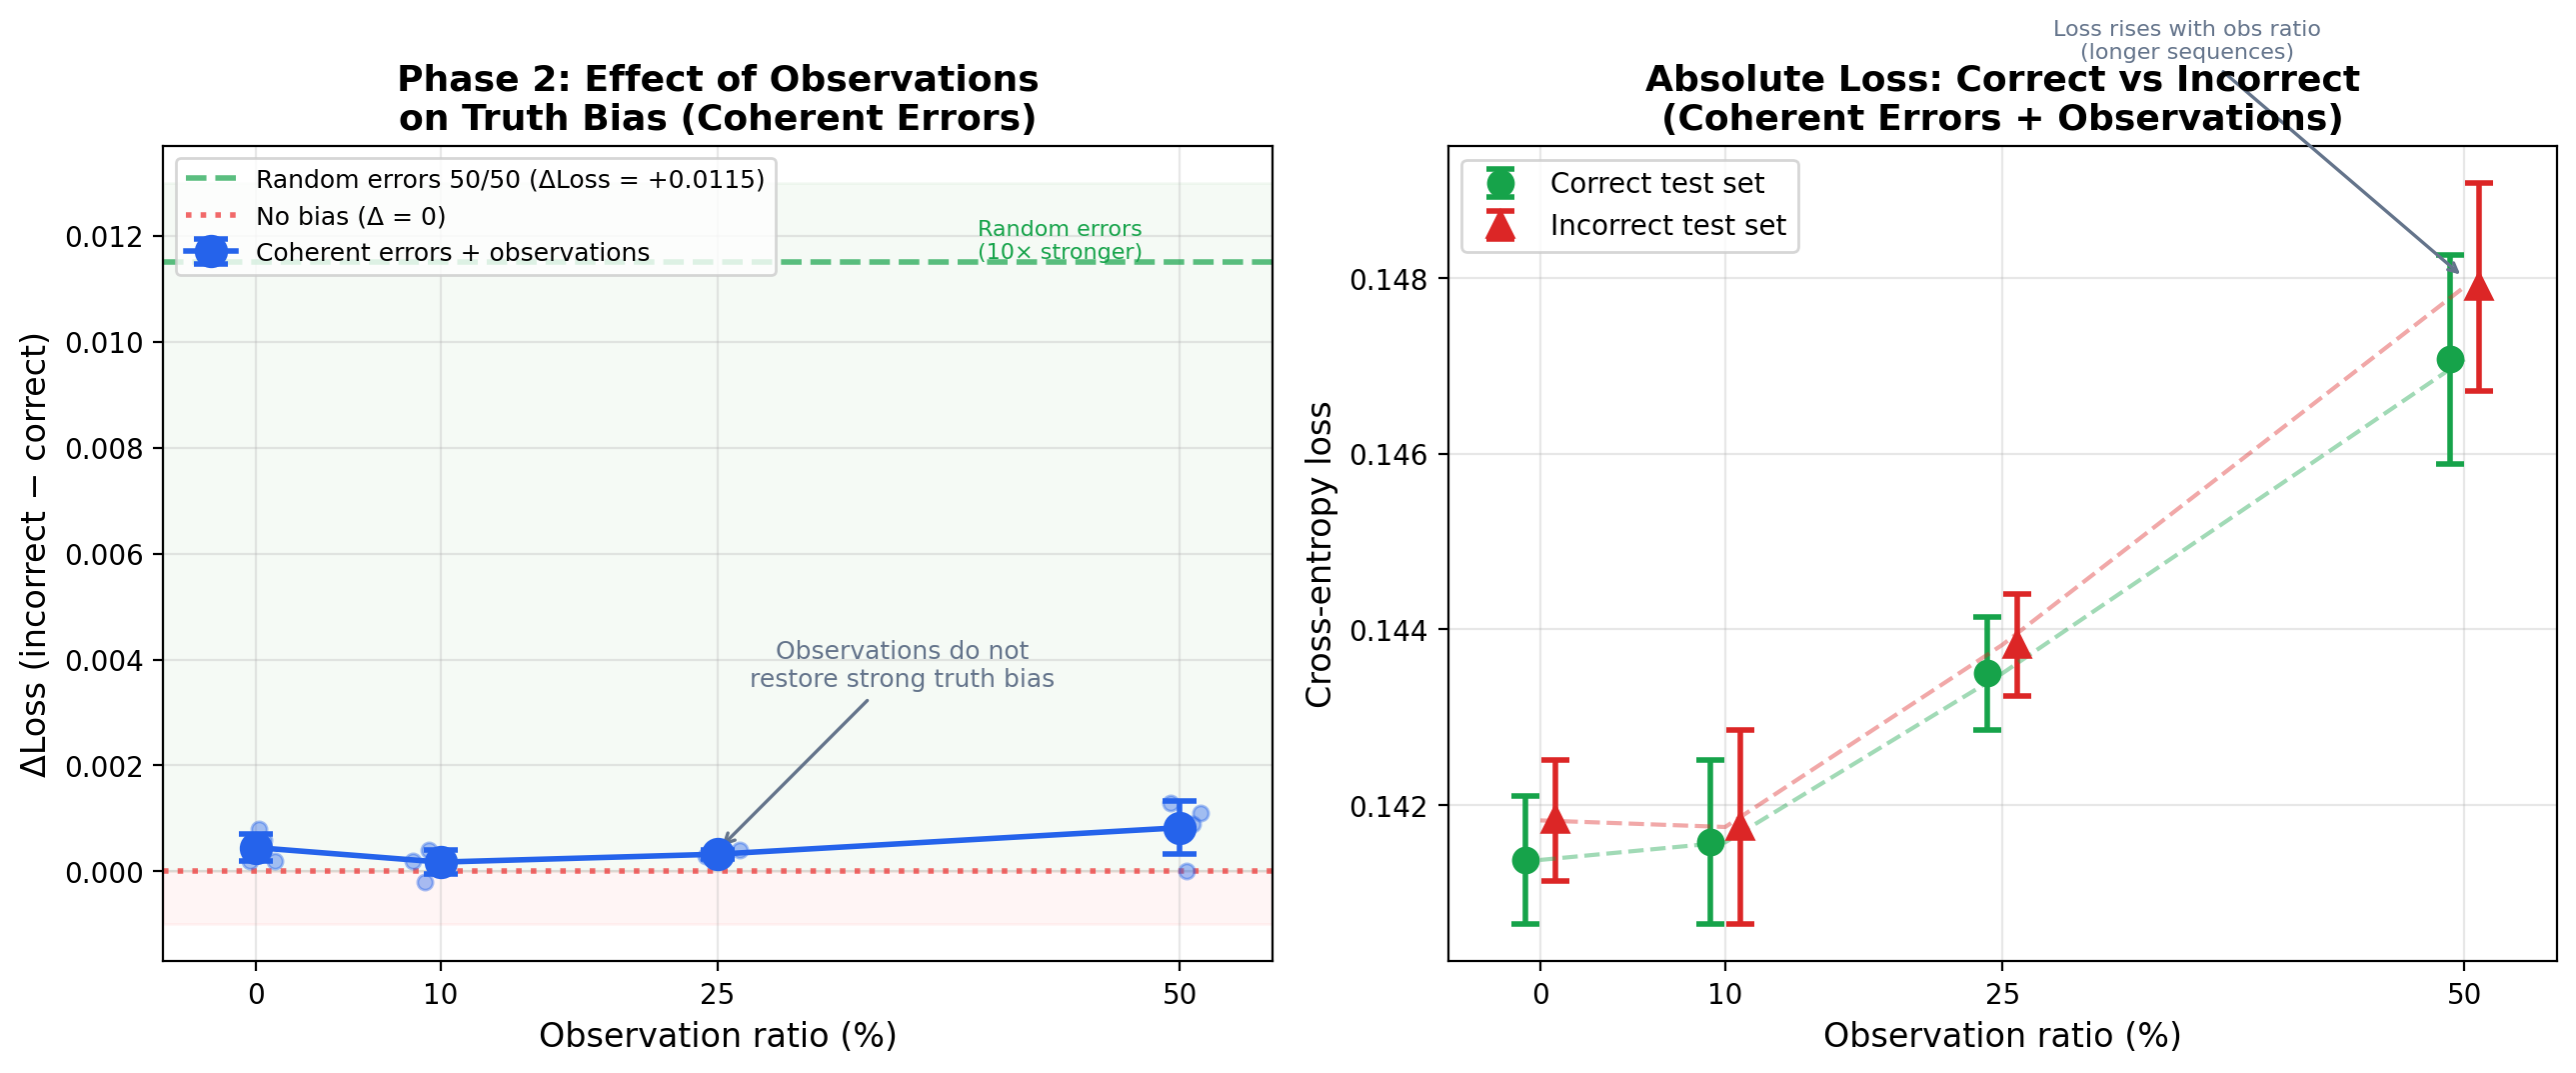
\includegraphics[keepaspectratio,alt={Figure 6}]{figure4_observations.png}}
\caption{Figure 6}
\end{figure}

\emph{Figure 6. DLoss as a function of the observation ratio. The effect
is an order of magnitude weaker than with random errors (+0.0115).}

\emph{*Note: the control condition (0\% observations) uses models from
Experiment 2, trained on a separately generated corpus with the same
50/50 ratio. Its DLoss = +0.0005 differs slightly from the -0.0004
reported for coherent errors in Table 2 (Experiment 1), because these
are different training corpora with different random problem instances.
Both values are within noise and consistent with the absence of truth
bias, as confirmed by paired evaluation (accuracy \textasciitilde49\%
for both model sets).}

\textbf{Result: the hypothesis is not supported.} Observations do not
restore strong truth bias. DLoss remains within the +0.0002 to +0.0008
range. The reason: discrepancies between the false theory and
observations are themselves \textbf{regular} (the a \ensuremath{\times} b = a \ensuremath{\times} (b\ensuremath{-}1) rule
always understates by a), and the model learns this regularity as an
additional rule.

The 100\% observations condition led to a loss explosion
(\textasciitilde0.32): the corpus became too complex for the tiny model
at 5000 steps. These results are excluded.

\subsection{6. Experiment 3: Informational Overhead of
Correction}\label{experiment-3-informational-overhead-of-correction}

\textbf{Hypothesis.} If bare discrepancies fail to produce a strong bias
due to their regularity, then ad hoc explanations -- unique for each
discrepancy -- should be incompressible and restore truth bias. Expected
ordering: C (ad hoc) \textgreater{} B (bare discrepancies)
\textgreater{} E (non-specific) \textgreater{} D (systematic correction)
\textasciitilde{} A (no observations).

Five conditions for the false theory (the correct theory is identical
across all):

\textbf{A: No observations} (baseline) -- theory without verification.

\textbf{B: Bare discrepancies} (Experiment 2, 50\% observations) --
theory with discrepancies.

\textbf{C: Ad hoc correction} -- a unique explanation for each
discrepancy:

\begin{verbatim}
Prediction: 10 \ensuremath{\times} 5 = 40. Observation: counted 50.
Explanation: In this case 5 is prime, so we add the base once more.
Corrected: 40 + 10 = 50 [check]
\end{verbatim}

Each Explanation is unique -- the model cannot compress them into a
single rule.

\textbf{D: Systematic correction} -- a single correction rule for all
discrepancies:

\begin{verbatim}
Correction rule: always add first operand.
Corrected: 40 + 10 = 50 [check]
\end{verbatim}

One rule for all problems -- compressible.

\textbf{E: Non-specific predictions} -- theory without a concrete
mapping:

\begin{verbatim}
Prediction: result is moderate. Observation: counted 50.
\end{verbatim}

\subsubsection{Results}\label{results}

To test whether conditions C/D/E produce transferable truth bias, we
begin with paired evaluation -- the most reliable metric, isolating
preference for correctness from textual confounds.

\textbf{Table 5a.} Paired evaluation of conditions C/D/E (coherent
pairs, 4 seeds).

{\def\LTcaptype{none} % do not increment counter
\begin{longtable}[]{@{}lccc@{}}
\toprule\noalign{}
Condition & Avg DLoss (paired) & Pair accuracy & Wilcoxon p \\
\midrule\noalign{}
\endhead
\bottomrule\noalign{}
\endlastfoot
C (ad hoc) & -0.0019 & 48.2\% & \textgreater0.3 \\
D (systematic) & -0.0011 & 49.7\% & \textgreater0.3 \\
E (non-specific) & -0.0007 & 49.6\% & \textgreater0.3 \\
\end{longtable}
}

\textbf{Paired evaluation reveals no truth bias for any of the C/D/E
conditions.} Pair accuracy \textasciitilde49\% -- at chance level.
Training with observations and correction \textbf{does not produce
transferable truth bias}: the model learns to process correction
patterns within the training corpus context, but does not transfer this
discrimination to pure mathematical pairs without observations.

\textbf{The corpus-level metric, by contrast, registers a non-zero
effect.} This divergence is methodologically significant:

\textbf{Table 5b.} Corpus-level DLoss across five conditions (tiny,
3.5M, 50/50, 4 seeds).

{\def\LTcaptype{none} % do not increment counter
\begin{longtable}[]{@{}
  >{\raggedright\arraybackslash}p{(\linewidth - 8\tabcolsep) * \real{0.1803}}
  >{\raggedright\arraybackslash}p{(\linewidth - 8\tabcolsep) * \real{0.2131}}
  >{\raggedright\arraybackslash}p{(\linewidth - 8\tabcolsep) * \real{0.1803}}
  >{\raggedright\arraybackslash}p{(\linewidth - 8\tabcolsep) * \real{0.1311}}
  >{\raggedright\arraybackslash}p{(\linewidth - 8\tabcolsep) * \real{0.2951}}@{}}
\toprule\noalign{}
\begin{minipage}[b]{\linewidth}\raggedright
Condition
\end{minipage} & \begin{minipage}[b]{\linewidth}\raggedright
Description
\end{minipage} & \begin{minipage}[b]{\linewidth}\raggedright
Avg DLoss
\end{minipage} & \begin{minipage}[b]{\linewidth}\raggedright
95\% CI
\end{minipage} & \begin{minipage}[b]{\linewidth}\raggedright
Seeds -\textgreater{} correct
\end{minipage} \\
\midrule\noalign{}
\endhead
\bottomrule\noalign{}
\endlastfoot
A & No observations & +0.0005 +/- 0.0003 & {[}+0.0002, +0.0007{]} &
4/4 \\
B & Bare discrepancies & +0.0008 +/- 0.0006 & {[}+0.0003, +0.0012{]} &
3/4 \\
E & Non-specific predictions & +0.0015 +/- 0.0009 & {[}+0.0008,
+0.0023{]} & 4/4 \\
C & Ad hoc correction & +0.0025 +/- 0.0008 & {[}+0.0020, +0.0033{]} &
4/4 \\
D & Systematic correction & +0.0026 +/- 0.0005 & {[}+0.0021, +0.0030{]}
& 4/4 \\
\end{longtable}
}

\begin{figure}
\centering
\pandocbounded{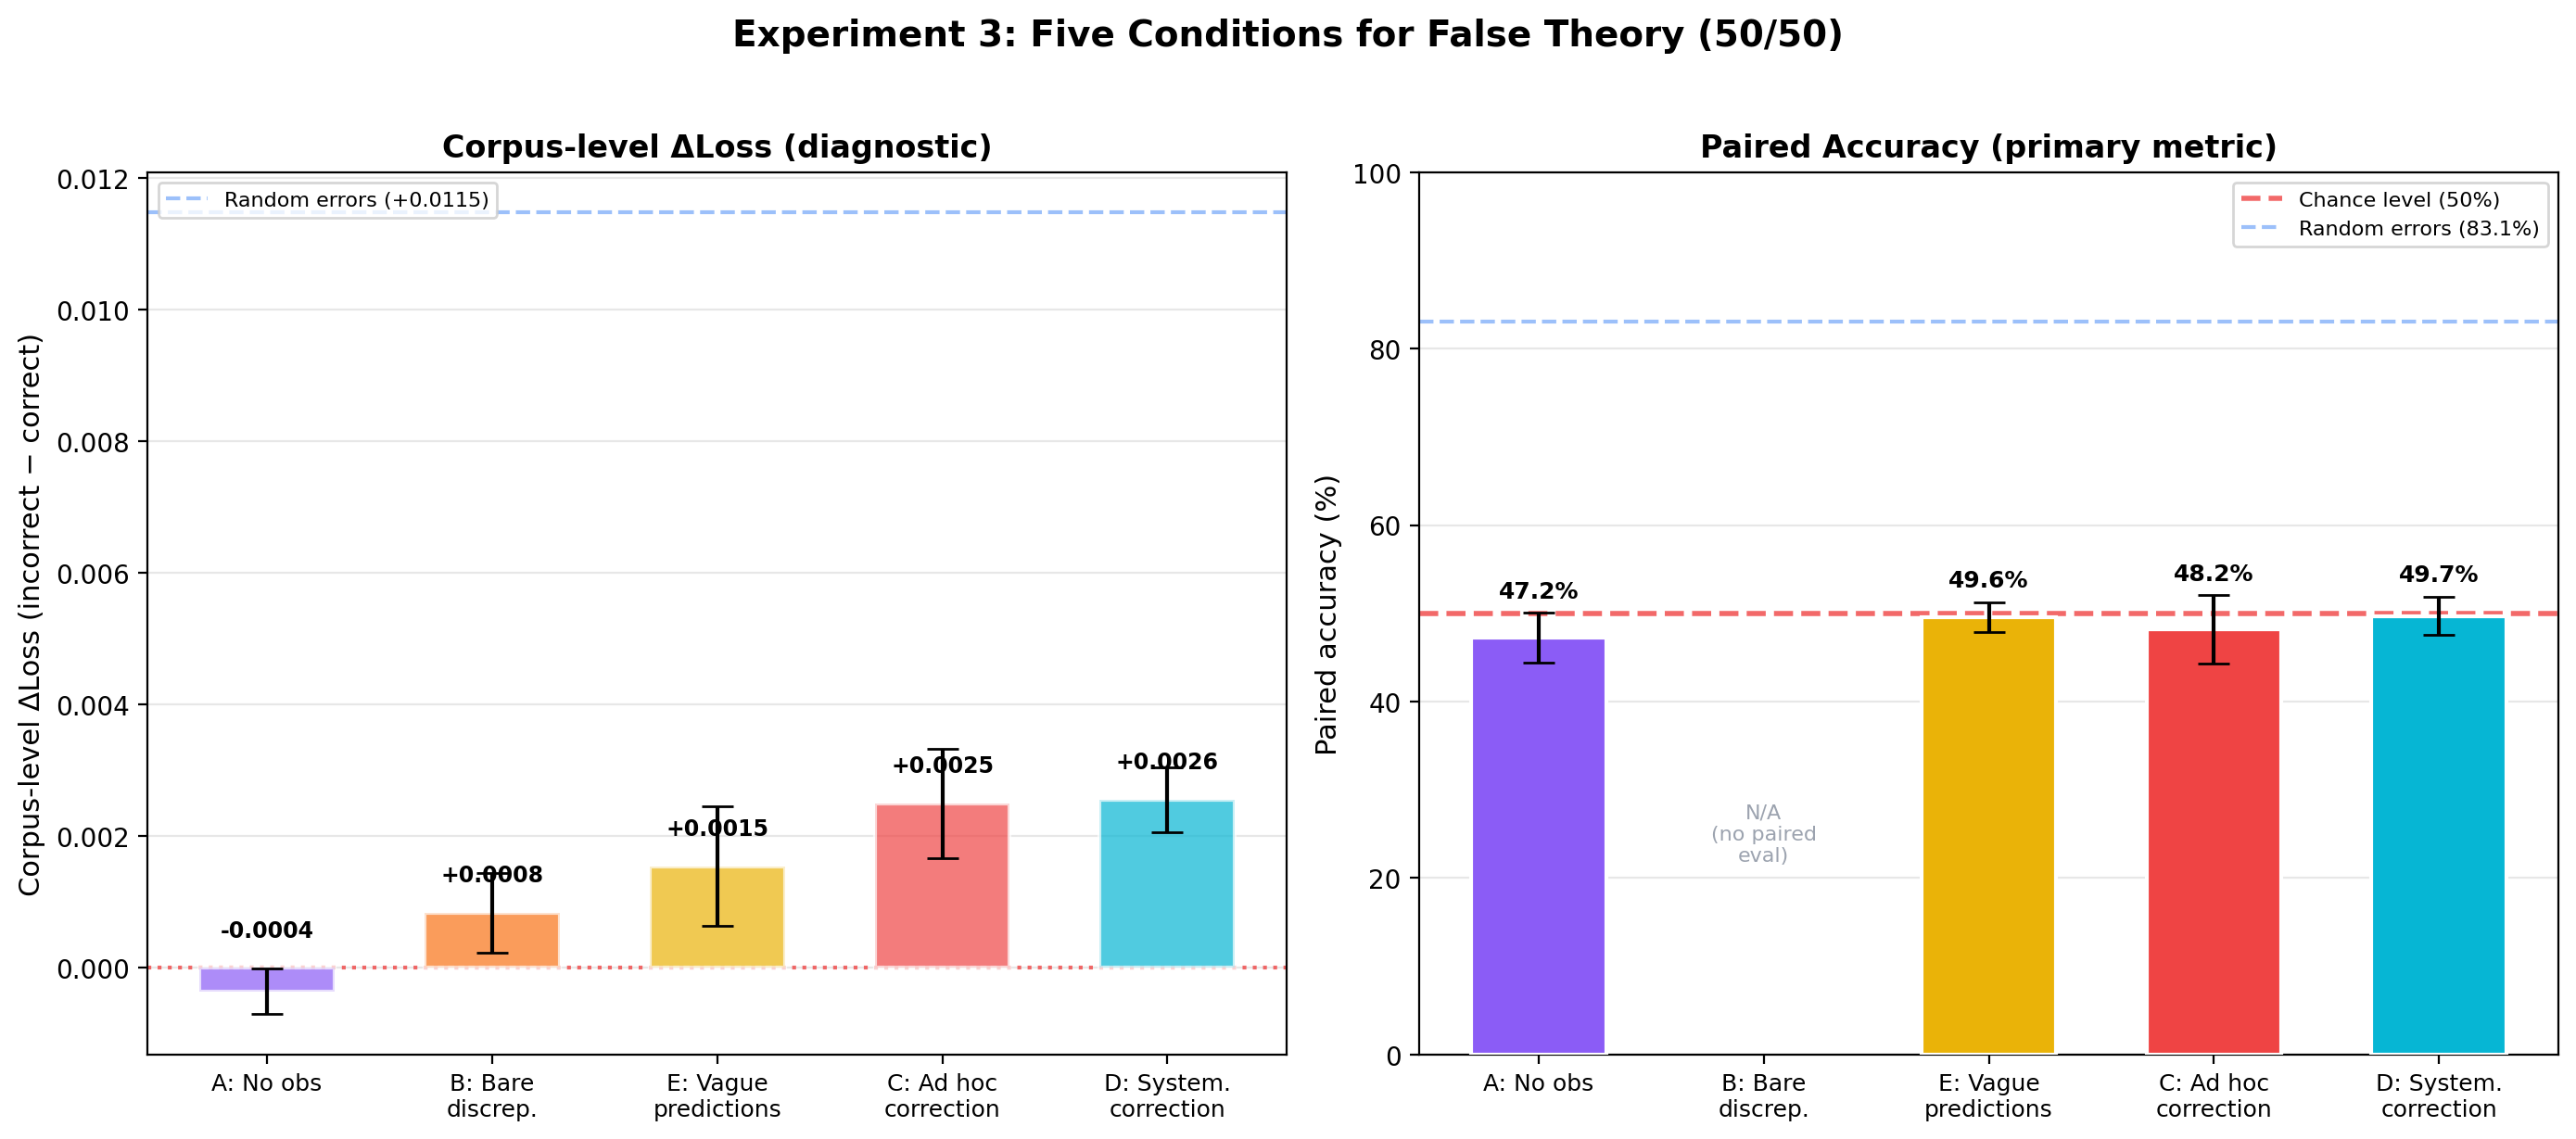
\includegraphics[keepaspectratio,alt={Figure 7}]{figure5_conditions.png}}
\caption{Figure 7}
\end{figure}

\emph{Figure 7. Corpus-level DLoss for five conditions. The ordering D
\textasciitilde{} C \textgreater{} E \textgreater{} B \textasciitilde{}
A does not reflect a preference for correctness, but is an artifact of
differences in text statistics (see Table 5a).}

The actual corpus-level ordering is D \textasciitilde{} C \textgreater{}
E \textgreater{} B \textasciitilde{} A. The predicted ordering (C
\textgreater{} B \textgreater{} E \textgreater{} D \textasciitilde{} A)
was partially confirmed: A \textasciitilde{} 0 and B \textless{} E
\textless{} C hold, but D \textasciitilde{} C instead of the expected D
\textasciitilde{} A. However, the divergence between corpus-level and
paired evaluation suggests that \textbf{most of the corpus-level effect
for conditions C/D/E is driven by differences in text statistics}
(different length and format of correct vs.~incorrect corpora), rather
than by preference for correctness given the same prompt.

\textbf{Caveat:} Absolute loss varies substantially (A: 0.14, B: 0.15,
C: 0.23, D: 0.24, E: 0.25), reflecting varying corpus lengths. Models
C/D/E are undertrained compared to A/B.

\textbf{Methodological takeaway.} This result demonstrates the
importance of paired evaluation: corpus-level DLoss can systematically
overestimate truth bias when correct and incorrect corpora differ in
format, length, or style. The only reliable source of truth bias is
\textbf{incoherence of the errors themselves} (Experiment 1, random
errors), confirmed by both metrics.

\subsection{7. Experiment 4: Scaling, Multi-Rule Errors, and Chained
Verification}\label{experiment-4-scaling-multi-rule-errors-and-chained-verification}

\textbf{Hypothesis.} If truth bias is driven by a structural advantage
in compression, then increasing model capacity may strengthen the effect
by improving learning of regularities. Coherent errors are expected to
remain difficult to distinguish from truth.

\subsubsection{7.1 Model Configurations}\label{model-configurations}

{\def\LTcaptype{none} % do not increment counter
\begin{longtable}[]{@{}lllll@{}}
\toprule\noalign{}
Size & Parameters & d\_model & Heads & Layers \\
\midrule\noalign{}
\endhead
\bottomrule\noalign{}
\endlastfoot
tiny & 3.5M & 256 & 4 & 4 \\
small & 11M & 384 & 6 & 6 \\
medium & 26M & 512 & 8 & 8 \\
large & 86M & 768 & 12 & 12 \\
\end{longtable}
}

All models trained for 5000 steps on the same corpus. Architecture:
GPT-2 (decoder-only transformer) with character-level tokenization.
Random-error and coherent scaling are both released with 4 seeds at each
size. Chained tasks use 2 large seeds due to computational constraints.

\subsubsection{7.2 Results: Fixed-Step Size Trend for Random
Errors}\label{results-fixed-step-size-trend-for-random-errors}

\textbf{Table 6.} Paired evaluation (random 50/50) by model size.

{\def\LTcaptype{none} % do not increment counter
\begin{longtable}[]{@{}
  >{\raggedright\arraybackslash}p{(\linewidth - 10\tabcolsep) * \real{0.0833}}
  >{\raggedright\arraybackslash}p{(\linewidth - 10\tabcolsep) * \real{0.1528}}
  >{\centering\arraybackslash}p{(\linewidth - 10\tabcolsep) * \real{0.2778}}
  >{\centering\arraybackslash}p{(\linewidth - 10\tabcolsep) * \real{0.1944}}
  >{\centering\arraybackslash}p{(\linewidth - 10\tabcolsep) * \real{0.1944}}
  >{\centering\arraybackslash}p{(\linewidth - 10\tabcolsep) * \real{0.0972}}@{}}
\toprule\noalign{}
\begin{minipage}[b]{\linewidth}\raggedright
Size
\end{minipage} & \begin{minipage}[b]{\linewidth}\raggedright
Parameters
\end{minipage} & \begin{minipage}[b]{\linewidth}\centering
Avg DLoss (paired)
\end{minipage} & \begin{minipage}[b]{\linewidth}\centering
Pair accuracy
\end{minipage} & \begin{minipage}[b]{\linewidth}\centering
Corpus DLoss
\end{minipage} & \begin{minipage}[b]{\linewidth}\centering
Seeds
\end{minipage} \\
\midrule\noalign{}
\endhead
\bottomrule\noalign{}
\endlastfoot
tiny & 3.5M & +0.048 & 83.1\% & +0.0115 & 4 \\
small & 11M & +0.063 & 88.4\% & +0.0129 & 4 \\
medium & 26M & +0.067 & 88.4\% & +0.0130 & 4 \\
large & 86M & +0.070 & 89.1\% & +0.0127 & 4 \\
\end{longtable}
}

\textbf{Table 6a.} Paired accuracy by problem type.

{\def\LTcaptype{none} % do not increment counter
\begin{longtable}[]{@{}lcccc@{}}
\toprule\noalign{}
Type & Tiny (3.5M) & Small (11M) & Medium (26M) & Large (86M) \\
\midrule\noalign{}
\endhead
\bottomrule\noalign{}
\endlastfoot
Algebra & 99.9\% & 100.0\% & 100.0\% & 100.0\% \\
Arithmetic & 95.2\% & 98.2\% & 98.6\% & 99.2\% \\
Derivatives & 72.4\% & 81.6\% & 82.4\% & 81.9\% \\
Equations & 65.9\% & 72.8\% & 72.1\% & 75.5\% \\
\end{longtable}
}

\begin{figure}
\centering
\pandocbounded{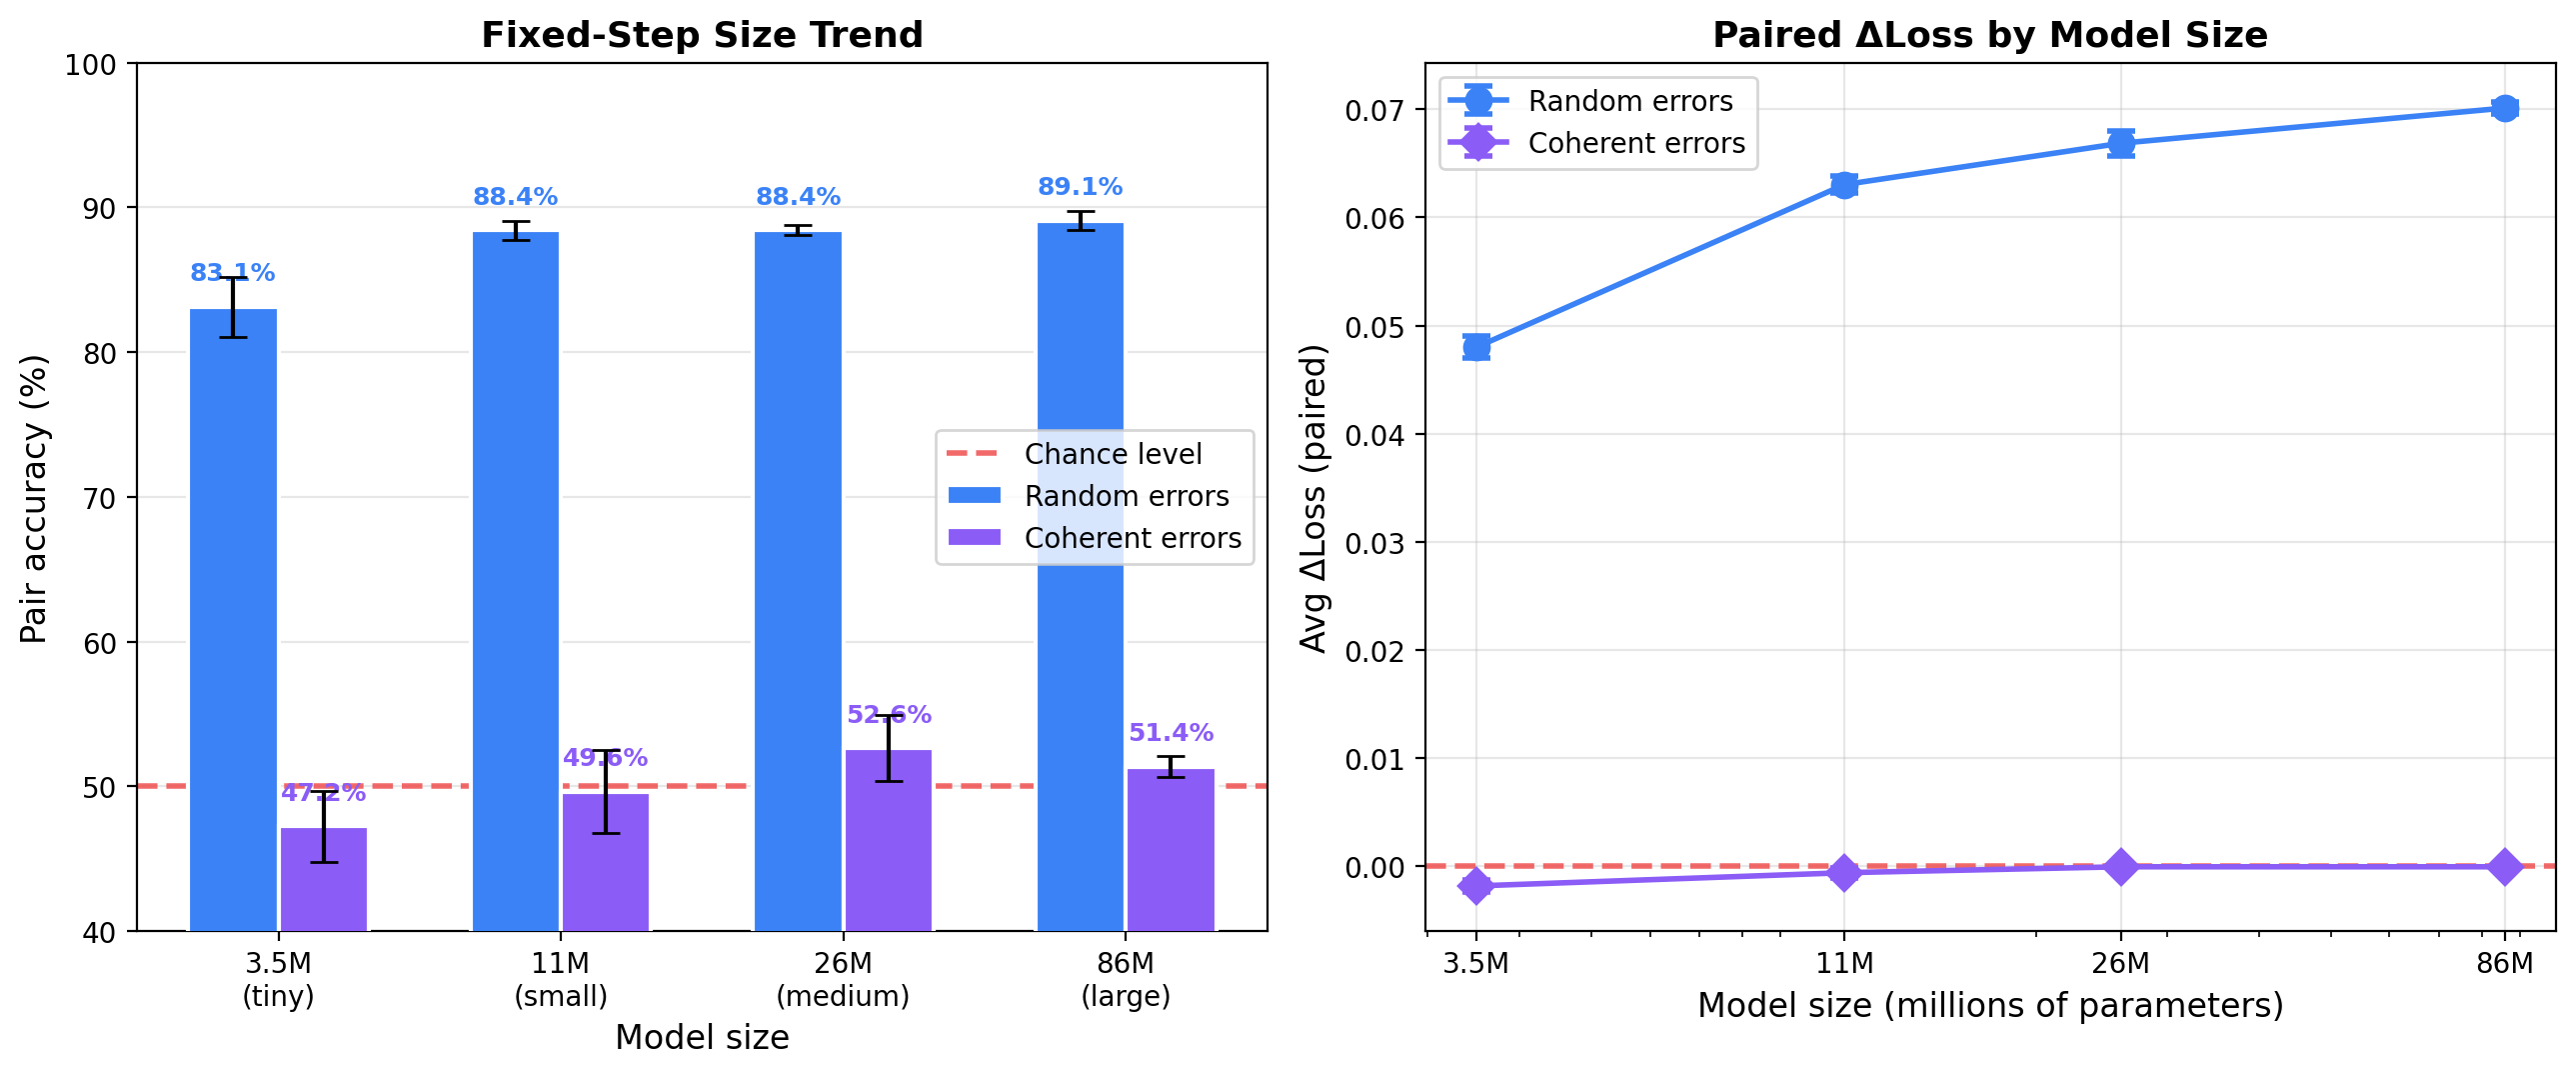
\includegraphics[keepaspectratio,alt={Figure 8}]{figure6_scaling.png}}
\caption{Figure 8}
\end{figure}

\emph{Figure 8. Fixed-step size trend. Left: pair accuracy rises from
83.1\% (tiny) to 89.1\% (large) for random errors, while coherent-error
accuracy stays near chance across the released
\texttt{3.5M}--\texttt{86M} runs. Right: paired DLoss by model size.}

In the available fixed-step runs, pair accuracy rises from 83.1\% (tiny)
to 89.1\% (large), with the largest gain between tiny and small. Between
small and medium, accuracy is nearly flat (88.4\% -\textgreater{}
88.4\%), and the large model adds a smaller further increase.
Improvement is concentrated in the harder problem types (derivatives and
equations), while algebra and arithmetic are already close to saturation
at small scale.

\textbf{Coherent errors still show no clear bias.} With full released
coverage, coherent pair accuracy remains close to chance across the
entire \texttt{3.5M}--\texttt{86M} range: \texttt{47.2\%} at tiny,
\texttt{49.6\%} at small, \texttt{52.6\%} at medium, and \texttt{51.4\%}
at large. Mean paired DLoss is correspondingly near zero at every size
(\texttt{-0.0018}, \texttt{-0.0006}, \texttt{-0.0001},
\texttt{-0.0001}). The coherent curve therefore does not show a clean
monotonic separation trend; under fixed-step training it stays
approximately flat around chance.

\textbf{Learning curves and behavioral convergence.} A potential
confound in fixed-step scaling is that larger models may be
undertrained: 86M parameters trained for 5000 steps may not have
converged. To address this, we evaluate paired accuracy at each saved
checkpoint (every 1000 steps) for all model sizes.

\begin{figure}
\centering
\pandocbounded{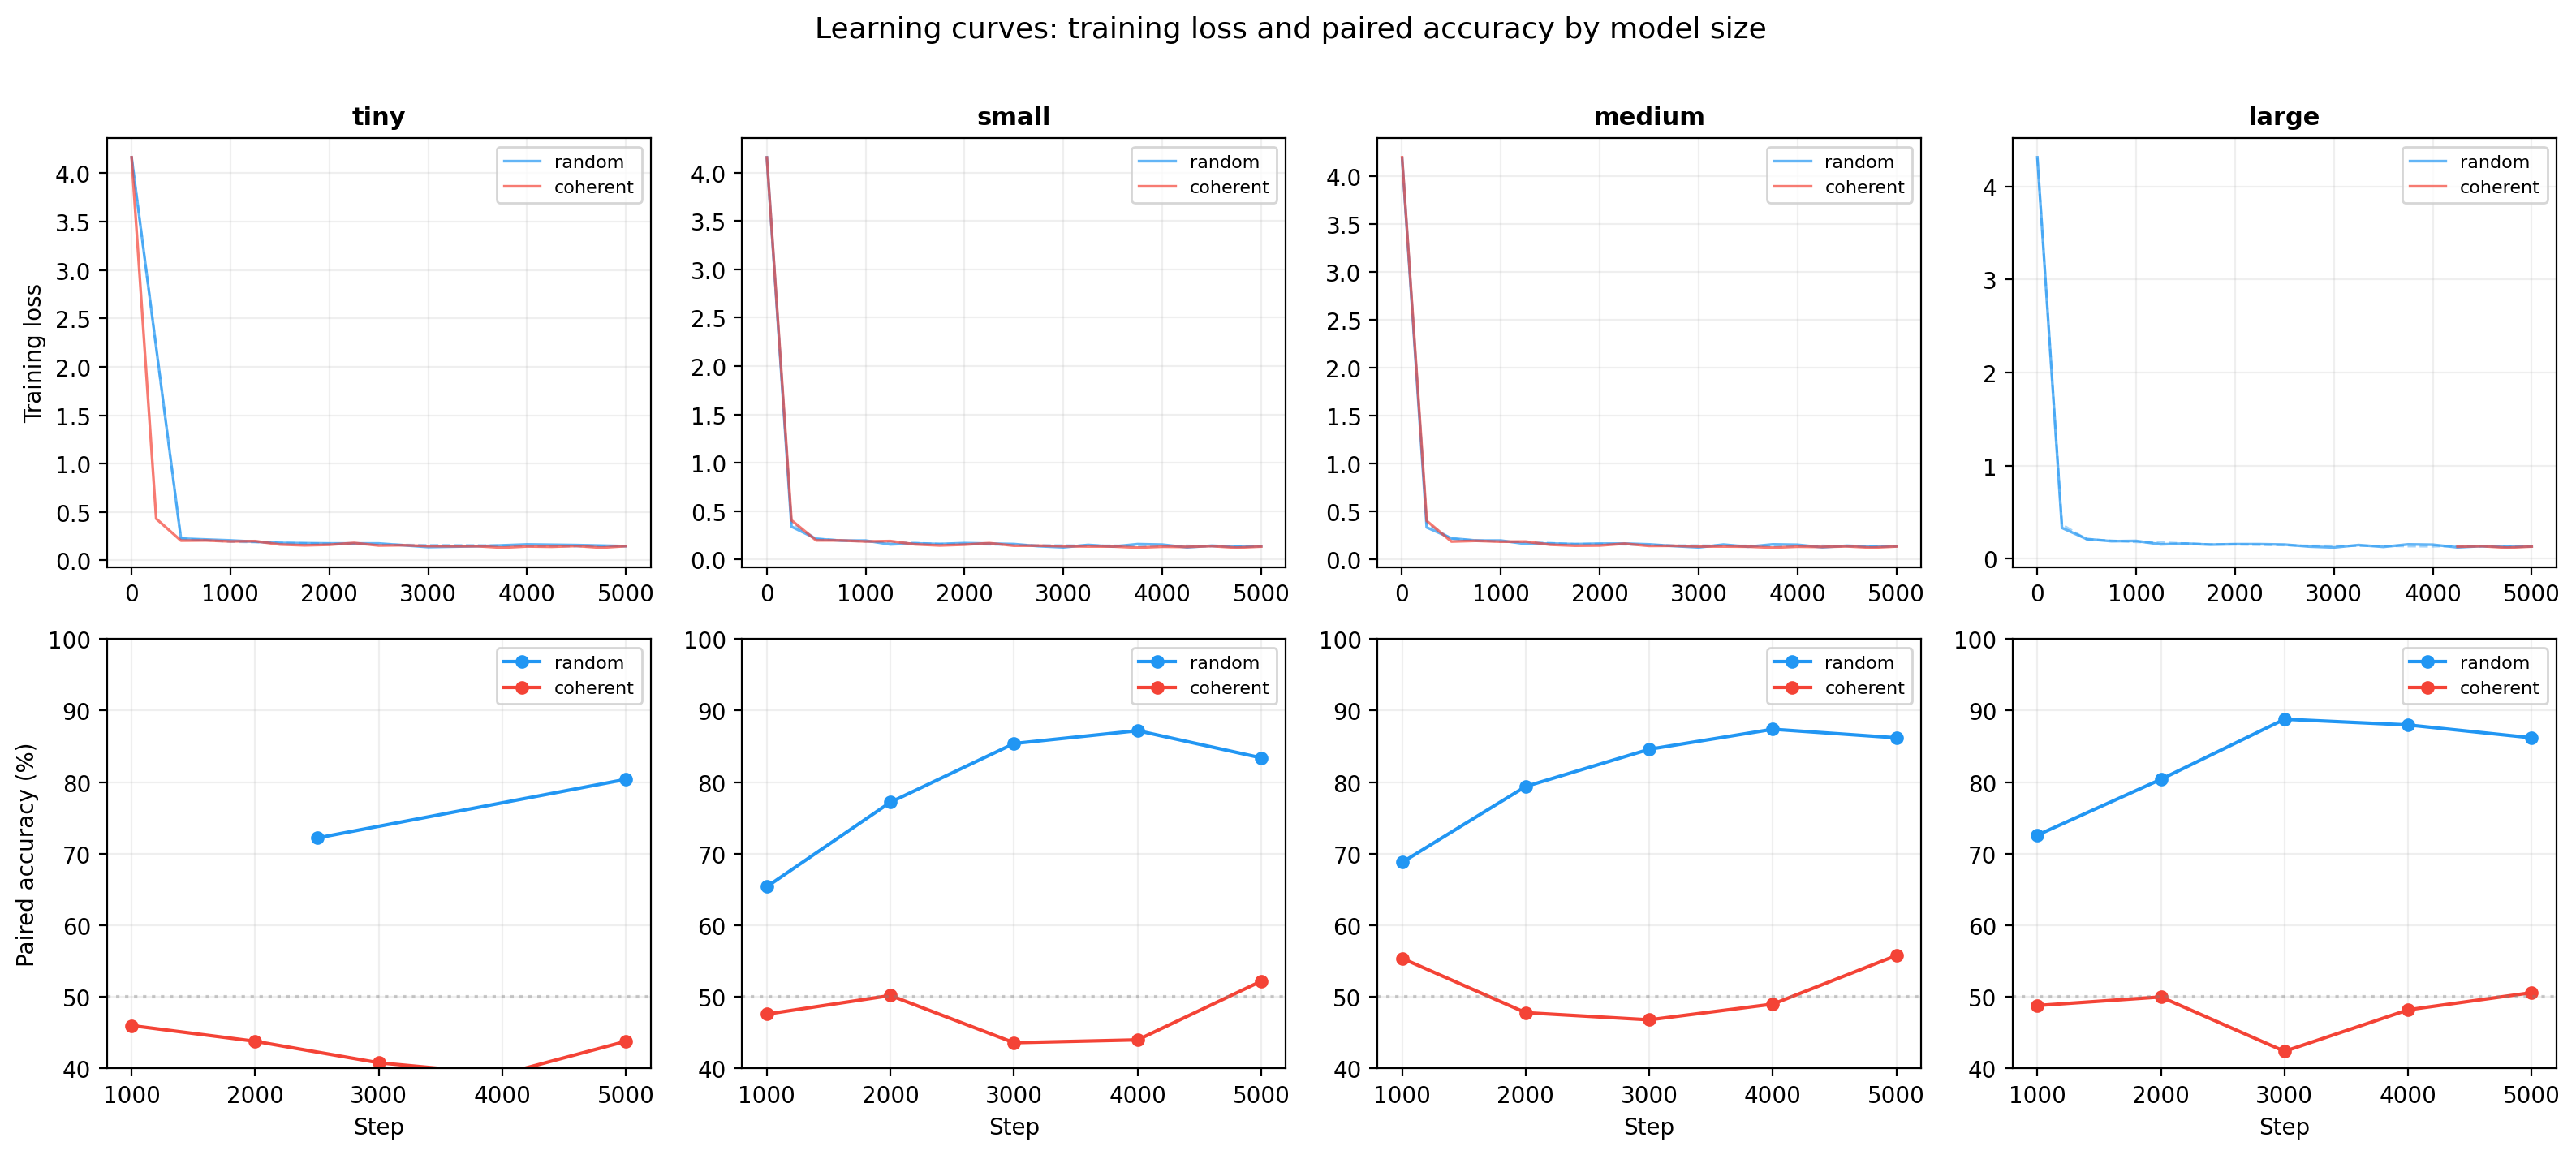
\includegraphics[keepaspectratio,alt={Figure 9}]{figure_learning_curves.png}}
\caption{Figure 9}
\end{figure}

\emph{Figure 9. Learning curves for all model sizes. Top: training loss
vs step. Bottom: paired accuracy vs step. Random-error models (blue)
show accuracy plateauing by step 3000--4000 at all sizes. Coherent-error
models (red) remain near chance throughout training.}

\textbf{Table LC1.} Paired accuracy at intermediate checkpoints (random
50/50, seed 42, 500-pair eval).

{\def\LTcaptype{none} % do not increment counter
\begin{longtable}[]{@{}lcccc@{}}
\toprule\noalign{}
Step & Tiny & Small & Medium & Large \\
\midrule\noalign{}
\endhead
\bottomrule\noalign{}
\endlastfoot
1000 & -- & 65.4\% & 68.8\% & 72.6\% \\
2000 & -- & 77.2\% & 79.4\% & 80.4\% \\
2500 & 72.2\% & -- & -- & -- \\
3000 & -- & 85.4\% & 84.6\% & 88.8\% \\
4000 & -- & 87.2\% & 87.4\% & 88.0\% \\
5000 & 80.4\% & 83.4\% & 86.2\% & 86.2\% \\
\end{longtable}
}

All sizes reach a behavioral plateau by step 3000--4000: paired accuracy
stabilizes or shows only minor fluctuation thereafter. The large model
achieves 88.8\% at step 3000 and remains within 2 percentage points
through step 5000. Coherent-error models show no trend at any
checkpoint, remaining within 40--56\% across all steps and sizes. This
rules out the hypothesis that the large model is substantially
undertrained: its behavioral convergence precedes the fixed training
endpoint, and the convergence-matched scaling concern (Section 8.4) is
therefore mitigated without requiring additional training runs.

\textbf{Scaling summary.} Under fixed-step training (5000 steps for all
sizes), the released random-error runs show a positive size trend in the
\texttt{3.5M}--\texttt{86M} range, while the released coherent runs
remain near chance across the same size range. Learning curves confirm
that behavioral convergence is reached before the 5000-step endpoint at
all sizes, so the observed size trend reflects capacity differences
rather than differential convergence. The safer conclusion remains that,
under this training setup, larger random-error models show stronger
paired preference for correct completions, whereas coherent falsehood
remains difficult to distinguish from truth.

\subsubsection{7.3 Experiment 5: Multi-Rule (Conspiratorial)
Errors}\label{experiment-5-multi-rule-conspiratorial-errors}

Experiments 1 and 4 established two poles: coherent errors (one rule per
task type) yield near-chance paired accuracy, while random errors yield
strong preference for correct completions. The question is what happens
in between.

We introduce \emph{multi-rule errors}: for each task type, a pool of N
alternative wrong rules is created, and for each problem, one rule is
chosen at random. Each rule is itself compact, but the mapping ``problem
-\textgreater{} rule'' is unpredictable. Conceptually, this should
increase the description length of the false system relative to the
one-rule coherent case.

\textbf{Table 7.} Matched paired evaluation of multi-rule errors (tiny,
3.5M, 50/50, 4 seeds).

{\def\LTcaptype{none} % do not increment counter
\begin{longtable}[]{@{}
  >{\centering\arraybackslash}p{(\linewidth - 8\tabcolsep) * \real{0.1364}}
  >{\centering\arraybackslash}p{(\linewidth - 8\tabcolsep) * \real{0.1818}}
  >{\centering\arraybackslash}p{(\linewidth - 8\tabcolsep) * \real{0.2879}}
  >{\centering\arraybackslash}p{(\linewidth - 8\tabcolsep) * \real{0.2121}}
  >{\centering\arraybackslash}p{(\linewidth - 8\tabcolsep) * \real{0.1818}}@{}}
\toprule\noalign{}
\begin{minipage}[b]{\linewidth}\centering
N rules
\end{minipage} & \begin{minipage}[b]{\linewidth}\centering
Avg Accuracy
\end{minipage} & \begin{minipage}[b]{\linewidth}\centering
Avg DLoss (paired)
\end{minipage} & \begin{minipage}[b]{\linewidth}\centering
Range of seed bootstrap CIs for DLoss
\end{minipage} & \begin{minipage}[b]{\linewidth}\centering
Wilcoxon p
\end{minipage} \\
\midrule\noalign{}
\endhead
\bottomrule\noalign{}
\endlastfoot
1 (coherent baseline) & 46.6\% & -0.0019 & {[}-0.0032, -0.0005{]} &
\textasciitilde1.0 \\
2 & 77.6\% & +0.0152 & {[}+0.0137, +0.0171{]} & \textless{} 10\^{}-6 \\
3 & 82.8\% & +0.0213 & {[}+0.0197, +0.0229{]} & \textless{} 10\^{}-6 \\
5 & 84.8\% & +0.0293 & {[}+0.0271, +0.0310{]} & \textless{} 10\^{}-6 \\
10 & 88.3\% & +0.0440 & {[}+0.0413, +0.0462{]} & \textless{} 10\^{}-6 \\
inf (random benchmark) & 83.1\% & +0.0480 & {[}+0.0460, +0.0500{]} &
\textless{} 10\^{}-6 \\
\end{longtable}
}

\begin{figure}
\centering
\pandocbounded{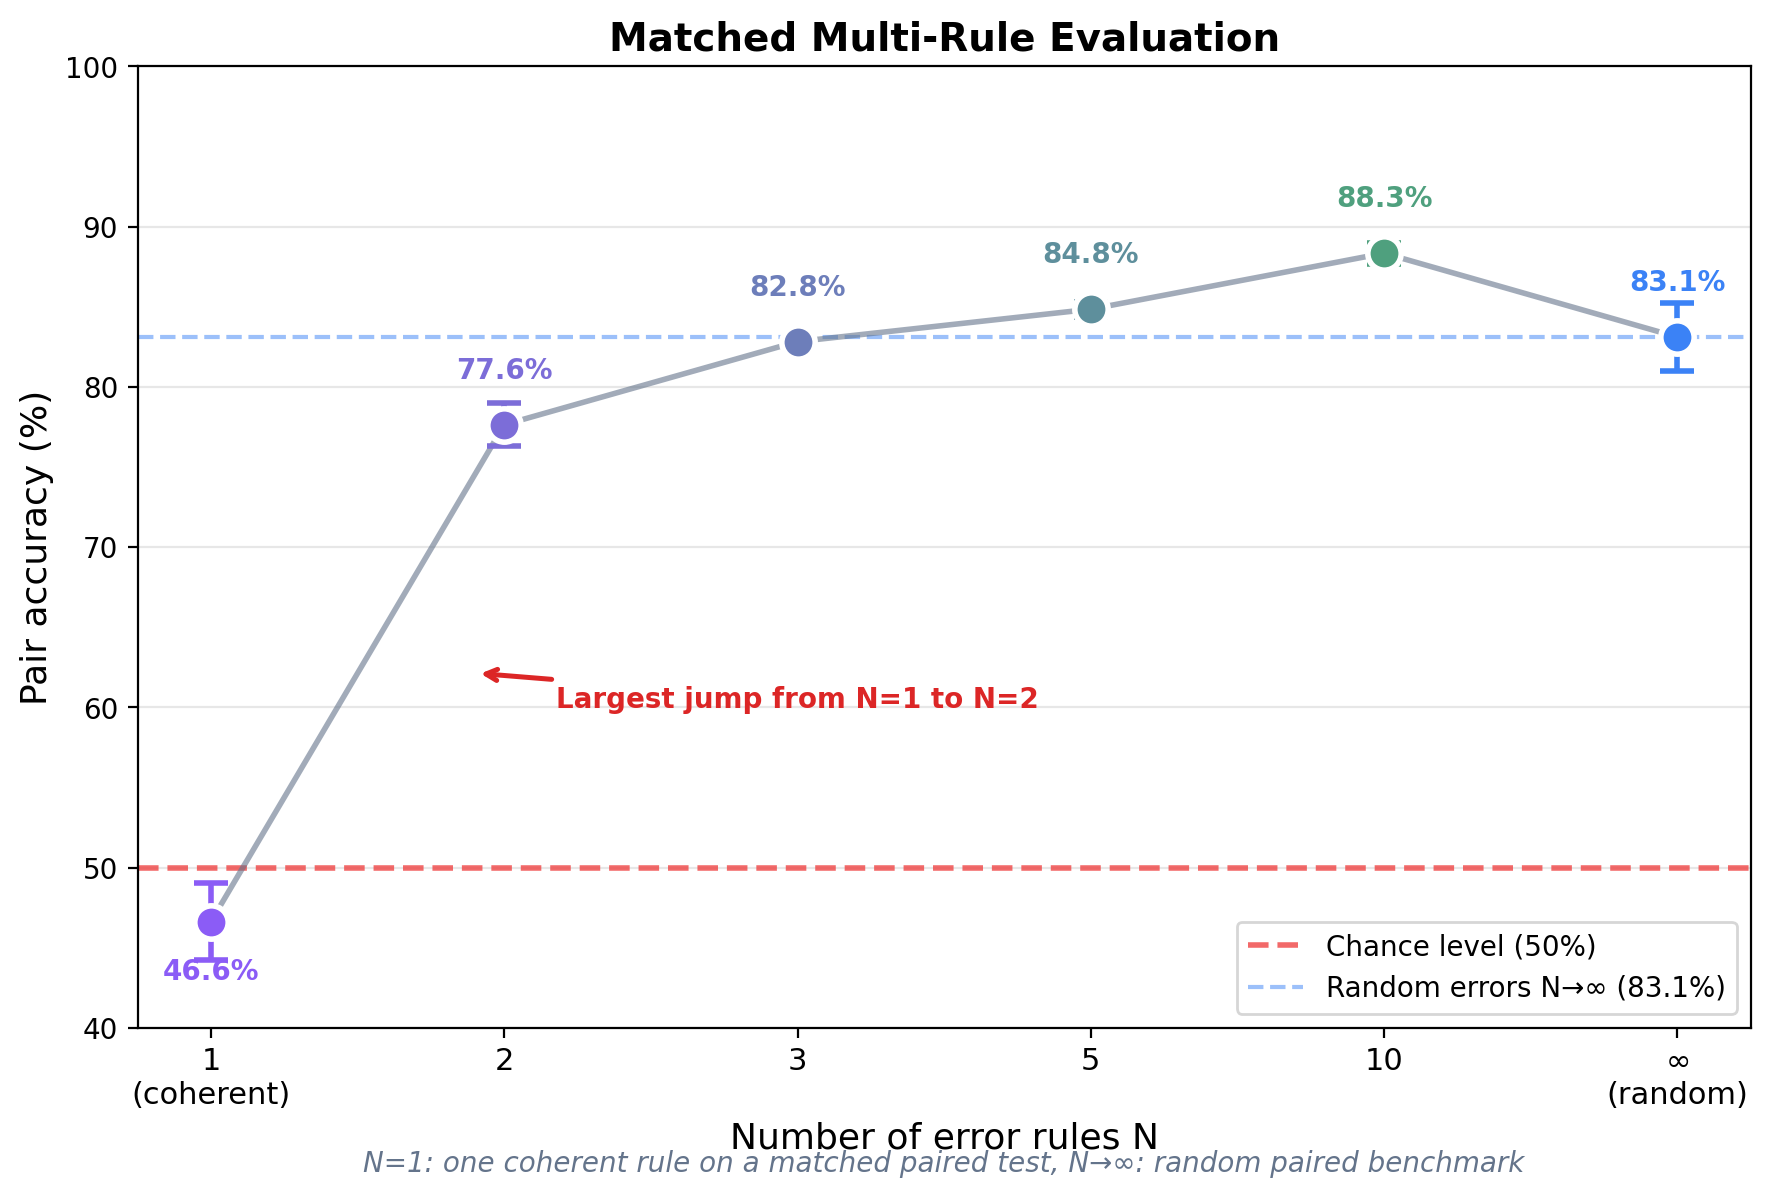
\includegraphics[keepaspectratio,alt={Figure 10}]{figure7_multirule.png}}
\caption{Figure 10}
\end{figure}

\emph{Figure 10. Matched paired evaluation for multi-rule errors. The
coherent baseline (\texttt{N=1}) is evaluated on a matched one-rule
paired test, and each \texttt{N\ \textgreater{}=\ 2} condition is
evaluated on its own multi-rule paired benchmark. The resulting curve is
steepest between \texttt{N=1} and \texttt{N=2}, but then continues to
grow gradually rather than exhibiting a single discontinuous jump.}

Three observations follow from the matched evaluation:

\begin{enumerate}
\def\labelenumi{\arabic{enumi}.}
\item
  \textbf{The effect is real under matched evaluation.} Evaluating each
  multi-rule condition on its own paired benchmark yields 46.6\% at
  \texttt{N=1}, 77.6\% at \texttt{N=2}, and 88.3\% at \texttt{N=10}.
  Comparing multi-rule models against a single-rule paired test (as done
  in the initial analysis) would overstate the effect by mixing
  evaluation families; matched tests are therefore used throughout.
\item
  \textbf{The largest increase is between one rule and two rules, but
  the curve remains graded.} The move from \texttt{N=1} to \texttt{N=2}
  produces the biggest change, yet additional rules continue to
  strengthen the effect
  (\texttt{77.6\%\ -\textgreater{}\ 82.8\%\ -\textgreater{}\ 84.8\%\ -\textgreater{}\ 88.3\%}).
\item
  \textbf{Multi-rule errors do not dominate the random benchmark at
  every \texttt{N}.} At \texttt{N=2}, the matched result is weaker than
  the random benchmark (77.6\% vs 83.1\%). By \texttt{N=10}, it exceeds
  the tiny random benchmark numerically, but the correct interpretation
  is not ``multi-rule is always harder than random.'' It is that
  increasing rule diversity can progressively erode the compressibility
  advantage of the false system.
\end{enumerate}

Three additional experiments -- a synthetic natural-language world
(Experiment 6), multi-alternative errors in natural language (Experiment
7), and cross-domain falsification with separate task types (Experiment
8) -- are reported in Appendix B. In brief: truth bias appears in
natural language but is substantially weaker (57.7\% vs 83.1\%); natural
language seems to absorb contradictions that would be easier to detect
in formal mathematics; and cross-domain data may selectively weaken the
coherence of false rules, though the effect is weak and non-monotonic.
These results extend the picture but are not required for the main
argument.

\subsubsection{7.4 Experiment 9: Chained Tasks with
Verification}\label{experiment-9-chained-tasks-with-verification}

A preliminary cross-domain experiment (Appendix B.3) showed that adding
separate correct tasks can destroy coherence, but the mechanism was
indirect. A stronger test is to embed the dependency \emph{within} the
task itself.

We construct \emph{chained tasks} in which a computation using the
coherent false rule (step A) is accompanied by arithmetic verification
(step B). For correct solutions, verification confirms the result
(residual = 0); for coherent-error solutions, it produces an
unpredictable numerical residual depending on specific problem
parameters. Six chain types:

\begin{itemize}
\tightlist
\item
  \textbf{Arithmetic -\textgreater{} reverse:} compute a chain of
  operations, then undo each step.
\item
  \textbf{Factoring -\textgreater{} evaluation:} factor an expression,
  then evaluate both sides at x = k.
\item
  \textbf{Linear equation -\textgreater{} back-substitution:} solve for
  x, substitute back.
\item
  \textbf{Quadratic equation -\textgreater{} root substitution:} find
  roots via Vieta's formulas, substitute.
\item
  \textbf{Derivative -\textgreater{} finite difference:} compute f'(a),
  compare with {[}f(a+h) - f(a){]}/h.
\item
  \textbf{Tangent -\textgreater{} prediction:} construct the tangent
  line, verify prediction at a nearby point.
\end{itemize}

The key distinction from the cross-domain experiment (Appendix B.3): the
model sees \emph{one} rule system, but with a verification step that
transforms the coherent error into an incompressible numerical residual
\emph{within} each task.

\textbf{Table 8.} Chained tasks (tiny, 3.5M, 50/50, 4 seeds). Paired
evaluation: correct vs coherent-error chains.

{\def\LTcaptype{none} % do not increment counter
\begin{longtable}[]{@{}
  >{\centering\arraybackslash}p{(\linewidth - 8\tabcolsep) * \real{0.0845}}
  >{\centering\arraybackslash}p{(\linewidth - 8\tabcolsep) * \real{0.2817}}
  >{\centering\arraybackslash}p{(\linewidth - 8\tabcolsep) * \real{0.0986}}
  >{\centering\arraybackslash}p{(\linewidth - 8\tabcolsep) * \real{0.1690}}
  >{\centering\arraybackslash}p{(\linewidth - 8\tabcolsep) * \real{0.3662}}@{}}
\toprule\noalign{}
\begin{minipage}[b]{\linewidth}\centering
Seed
\end{minipage} & \begin{minipage}[b]{\linewidth}\centering
Accuracy (chained)
\end{minipage} & \begin{minipage}[b]{\linewidth}\centering
DLoss
\end{minipage} & \begin{minipage}[b]{\linewidth}\centering
Wilcoxon p
\end{minipage} & \begin{minipage}[b]{\linewidth}\centering
Accuracy (coherent ctrl)
\end{minipage} \\
\midrule\noalign{}
\endhead
\bottomrule\noalign{}
\endlastfoot
42 & 71.4\% & +0.0116 & \textless{} 10\^{}-6 & 43.1\% \\
43 & 70.0\% & +0.0112 & \textless{} 10\^{}-6 & 47.5\% \\
44 & 72.5\% & +0.0118 & \textless{} 10\^{}-6 & 41.3\% \\
45 & 69.8\% & +0.0116 & \textless{} 10\^{}-6 & 41.4\% \\
\textbf{Avg} & \textbf{70.9\%} & \textbf{+0.0115} & -- &
\textbf{43.3\%} \\
\end{longtable}
}

\textbf{Table 8a.} Accuracy by chain type (averaged over 4 seeds).

{\def\LTcaptype{none} % do not increment counter
\begin{longtable}[]{@{}lcc@{}}
\toprule\noalign{}
Chain type & Accuracy & n \\
\midrule\noalign{}
\endhead
\bottomrule\noalign{}
\endlastfoot
Arithmetic (forward + reverse) & 95.8\% & 824 \\
Factoring (factor + evaluate) & 89.9\% & 843 \\
Linear equation (solve + substitute) & 88.2\% & 879 \\
Quadratic (roots + substitute) & 60.5\% & 869 \\
Derivative (power rule + finite diff) & 53.4\% & 784 \\
Tangent (slope + predict) & 34.8\% & 801 \\
\end{longtable}
}

\begin{figure}
\centering
\pandocbounded{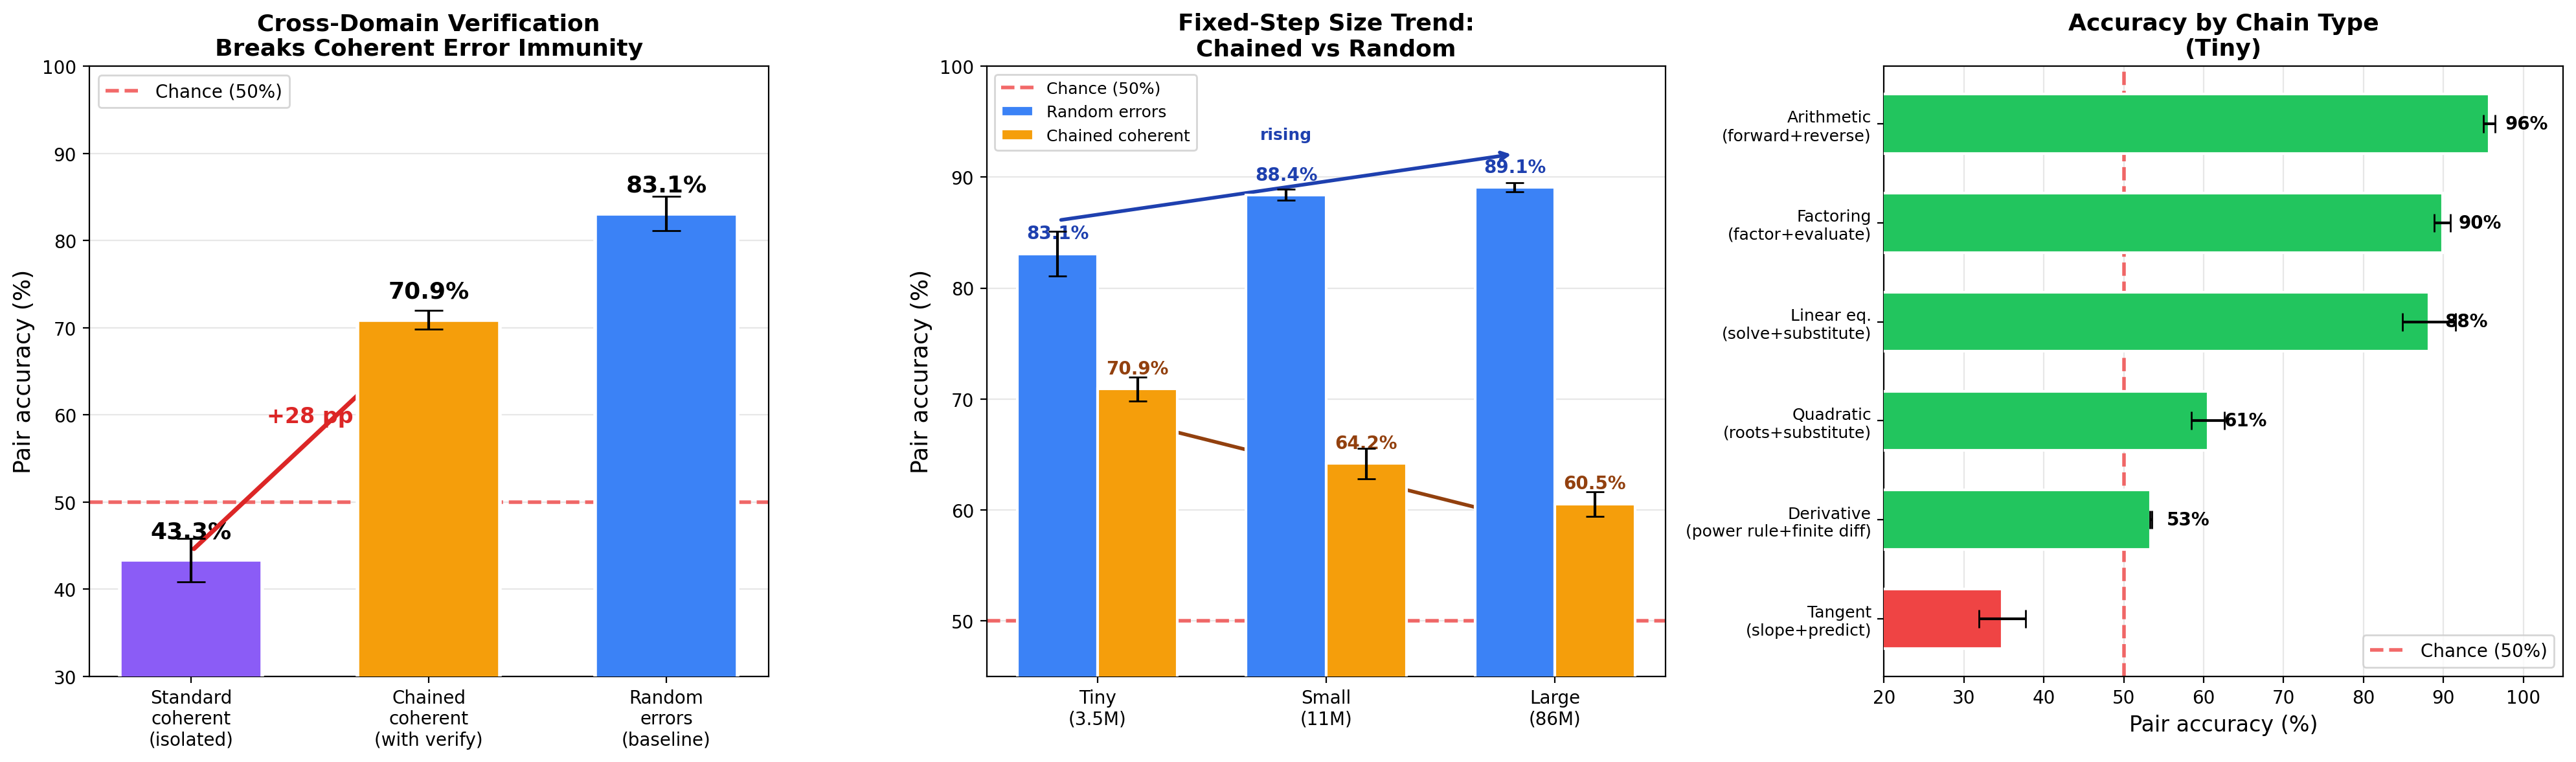
\includegraphics[keepaspectratio,alt={Figure 11}]{figure10_chained.png}}
\caption{Figure 11}
\end{figure}

\emph{Figure 11. Chained tasks. Left: verification raises accuracy from
43\% (isolated coherent) to 71\% on the tiny model. Center: under
fixed-step training, the available chained-task runs show a declining
size trend (71\% -\textgreater{} 61\%), while random-error accuracy
rises (84\% -\textgreater{} 89\%). Right: accuracy by chain type
(tiny).}

\textbf{Table 8b.} Chained tasks scaling by model size.

{\def\LTcaptype{none} % do not increment counter
\begin{longtable}[]{@{}llcccc@{}}
\toprule\noalign{}
Size & Params & Seeds & Accuracy & DLoss & Trend \\
\midrule\noalign{}
\endhead
\bottomrule\noalign{}
\endlastfoot
Tiny & 3.5M & 4 & 70.9\% +/- 1.2\% & +0.0115 & -- \\
Small & 11M & 4 & 64.2\% +/- 1.5\% & +0.0090 & down \\
Large & 86M & 2 & 60.6\% +/- 1.2\% & +0.0078 & down \\
\end{longtable}
}

For comparison, random error scaling: tiny 83.1\% -\textgreater{} small
88.4\% -\textgreater{} large 89.1\% (up).

\textbf{Table 8c.} Control experiment: truncated chains (no verification
step).

{\def\LTcaptype{none} % do not increment counter
\begin{longtable}[]{@{}lcc@{}}
\toprule\noalign{}
Condition & Accuracy (tiny, 4 seeds) & p \\
\midrule\noalign{}
\endhead
\bottomrule\noalign{}
\endlastfoot
With verification (chained) & 70.9\% +/- 1.2\% & \textless{} 10\^{}-6 \\
Without verification (truncated) & 44.3\% +/- 2.1\% &
\textasciitilde1.0 \\
Standard coherent & 43.3\% +/- 2.9\% & \textasciitilde1.0 \\
\end{longtable}
}

The control experiment with truncated chains (same task types, but
without the verification step) suggests that the observed truth bias is
produced by verification rather than by task structure alone: accuracy
of truncated chains (44.3\%) is close to standard coherent errors
(43.3\%). In this setup, truth bias with coherent errors appears only
when verification is present.

Five key observations:

\begin{enumerate}
\def\labelenumi{\arabic{enumi}.}
\item
  \textbf{Verification restores truth bias.} Accuracy of 70.9\% (p
  \textless{} 10\^{}-6 for all 4 seeds) -- significantly above chance
  and above standard coherent errors (43.3\% on the same models
  evaluated on isolated tasks). Cross-domain dependencies transform
  coherent errors into incompressible ones.
\item
  \textbf{The control is consistent with the mechanism.} The same models
  evaluated on the standard coherent test (without verification) yield
  accuracy of 43.3\% -- below chance, as in Experiment 1. This supports
  the interpretation that the verification step, rather than task
  structure alone, is what produces truth bias here.
\item
  \textbf{The type spectrum reflects verification strength.} Arithmetic
  reverse (96\%) -- the strongest signal: with incorrect multiplication,
  reverse division yields a fraction instead of an integer. Tangent
  (35\%) -- the only type below chance: the O(h\^{}2) approximation
  error in finite differences masks the coherent rule error, and the
  model learns the pattern ``with error, the prediction is closer to
  zero.''
\item
  \textbf{The effect is substantial but incomplete.} Accuracy rises to
  70.9\% compared with 83.1\% for random errors. Verification therefore
  recovers a large share of the random-error advantage without
  eliminating the gap entirely. This suggests that sufficiently dense
  cross-domain dependencies could weaken the immunity of coherent
  falsehood, but the current setup does not show complete removal.
\item
  \textbf{Declining chained-task performance under fixed training
  steps.} Unlike random errors, chained tasks show a downward trend in
  the currently available runs: 70.9\% -\textgreater{} 64.2\%
  -\textgreater{} 60.6\%. This is consistent with the possibility that
  higher-capacity models learn the coherent within-domain pattern more
  readily than the weaker verification signal, but the evidence is still
  preliminary because the large model uses only 2 seeds and all sizes
  are trained for the same number of steps.
\end{enumerate}

\subsection{8. Discussion}\label{discussion}

\subsubsection{8.1 Unified Interpretation}\label{unified-interpretation}

The experiments support three main conclusions.

\textbf{A. Compression favors consistency, not truth.} Any internally
consistent rule system -- true or false -- compresses equally well.
Truth bias with random errors (83\% paired accuracy) is explained by the
fact that each random error must be memorized individually: random
incorrect completions are measurably harder to compress than correct
ones (gzip delta = +0.0012), while coherent incorrect completions are
equally compressible (delta \textasciitilde{} 0, accuracy
\textasciitilde{} 49\%). Multi-rule errors form a graded boundary:
increasing rule diversity from N=1 to N=10 progressively erodes the
compressibility advantage of the false system (compression delta: 0
-\textgreater{} +0.0076; accuracy: 47\% -\textgreater{} 88\%). The
compression ratio gap, measured by a generic compressor on raw text
without any trained model, predicts paired accuracy across 9 conditions
(Spearman rho = 0.68, p = 0.042). This is not a claim about truth in
general -- it is a claim about error structure in synthetic corpora.

\textbf{B. Paired evaluation is necessary; corpus-level metrics
mislead.} At 10/90, corpus-level DLoss inverts (-0.0016), but paired
accuracy remains robust (67\%). For conditions C/D/E, corpus-level DLoss
is positive, but paired accuracy is \textasciitilde49\%. The per-pair
NLL difference distribution reveals why: for random errors, the
distribution is right-skewed (mean = +0.048, median = +0.025) with a
heavy tail, so outlier pairs inflate the mean beyond what the majority
of pairs would suggest. For coherent errors, the distribution is
symmetric around zero. This explains the apparent metric divergence in
the synthetic world coherent condition (Appendix B.1): pair accuracy
46.6\% but mean DLoss +0.019. Observations and correction (Experiments
2--3) increase corpus-level DLoss but do not produce transferable truth
bias at the pair level -- the only reliable mechanism is error
incoherence itself.

\begin{figure}
\centering
\pandocbounded{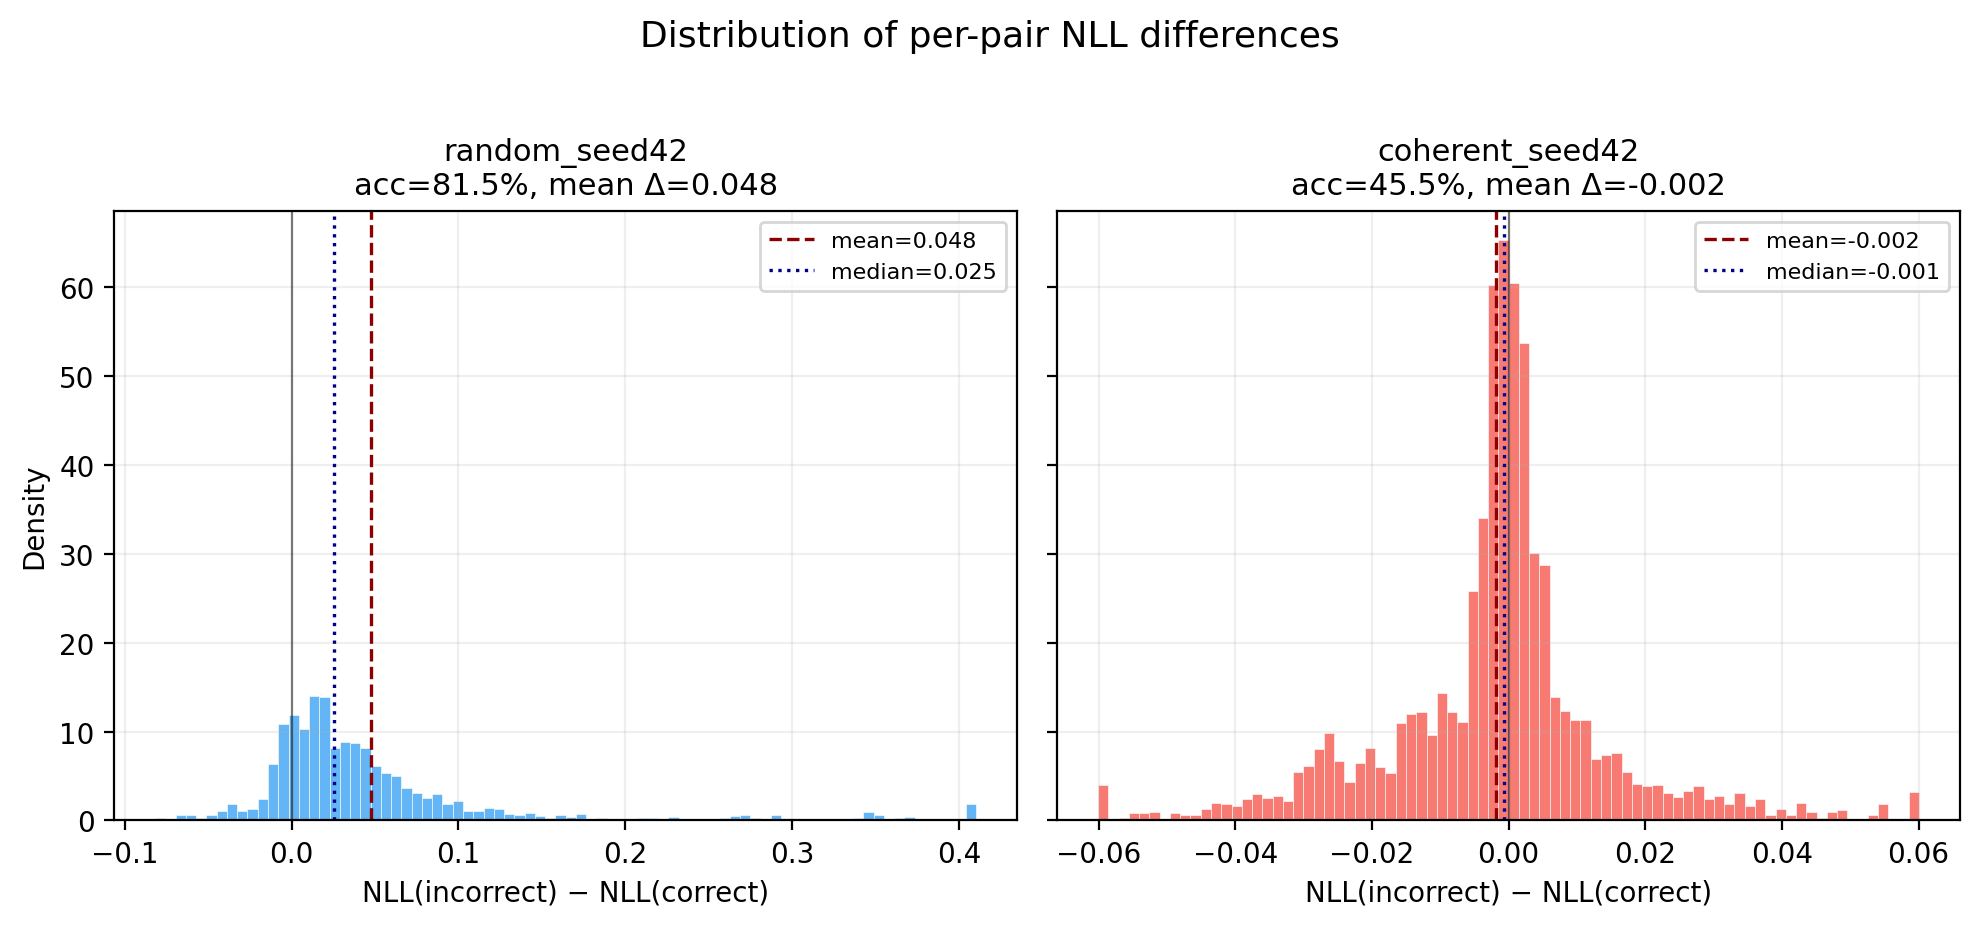
\includegraphics[keepaspectratio,alt={Figure 12}]{figure_nll_histogram.png}}
\caption{Figure 12}
\end{figure}

\emph{Figure 12. Distribution of per-pair NLL differences
(NLL(incorrect) - NLL(correct)) for random (left) and coherent (right)
error models. Random: right-skewed, 81.5\% of pairs positive, heavy tail
to +0.4. Coherent: symmetric around zero, 45.5\% positive.}

\textbf{C. Scaling, transfer, and the limits of verification.}
Random-error preference grows with model size (83\% -\textgreater{}
89\%, with learning curves confirming behavioral convergence by step
3000--4000 at all sizes), while coherent accuracy stays near chance
(47\%--53\%) across 3.5M--86M. Truth bias transfers to natural language
but weakens substantially (58\% vs 83\%), and the multi-alternative
natural-language curve rises much more slowly than the matched math
multi-rule curve. Chained tasks with embedded verification restore truth
bias from 43\% to 71\% at tiny scale, but the effect declines at larger
sizes (61\% at 86M) -- consistent with the idea that higher-capacity
models learn coherent within-domain patterns more readily than weak
verification signals. This declining trend is preliminary (2 seeds at
large) and should not be treated as an established inverse-scaling law.

\subsubsection{8.2 Analogy with Popper's
Falsifiability}\label{analogy-with-poppers-falsifiability}

Our results admit an interpretive analogy with the falsifiability
criterion (Popper, 1959). Compression pressure acts as a computational
analog: a true theory with concrete predictions requires no additional
explanations (maximal compression); a false theory whose predictions
diverge from data needs correction (poor compression); a theory with ad
hoc escape hatches expands with every observation (anti-compression).

However, the analogy has limits. First, the model does not ``test''
theories -- it simply minimizes code length. Second, our data show that
bare discrepancies alone barely help (condition B \textasciitilde{} A):
regular discrepancies are compressible. Popperian falsification assumes
that a discrepancy with observation refutes a theory; for a compressor
model, a discrepancy is merely another pattern. Moreover, paired
evaluation of conditions C/D/E showed that even ad hoc correction does
not produce transferable truth bias -- the model learns to process
correction patterns but does not transfer this to pure mathematical
pairs.

Practical analogies from the history of science are appropriate as
illustrations. The geocentric model required ever more epicycles to
reconcile with observations (a variation of condition C); phlogiston
theory needed special assumptions to explain mass increase during
combustion; miasma theory could not explain why disease spread along
waterways rather than by wind. However, our experiments use the
mathematical domain, and transfer to these real-world examples remains
an open question.

\subsubsection{8.3 Implications}\label{implications}

\textbf{For alignment.} The training objective does not by itself
provide a ``truth compass.'' Systematic falsehood can remain competitive
when internally coherent. Verification dependencies can help, but their
effectiveness at scale remains an open question.

\textbf{For understanding hallucinations.} Our results complement the
statistical hallucination bound of Kalai \& Vempala (2024) and the
compression-failure analysis of Chlon et al.~(2025): coherent
misconceptions can remain attractive to the model because they compress
well, independently of rarity. Whether this extends from synthetic
corpora to real hallucination behavior requires direct empirical work.

\subsubsection{8.4 Limitations}\label{limitations}

\textbf{Model scale and information-theoretic limits.} Experiments use
models from \texttt{3.5M} to \texttt{86M} parameters. The released
fixed-step runs show stronger random-error preference at larger sizes,
while coherent isolated falsehood remains near chance across the same
range. Chained tasks show a declining trend, not a settled
inverse-scaling result. Extrapolation to larger models requires further
experiments.

For \emph{isolated} coherent errors, there is a stronger heuristic
argument. If the false system has comparable description length to the
true system (one rule vs.~one rule) and both appear at equal frequency,
an idealized MDL learner would have little basis to prefer one over the
other. The released artifacts are consistent with near-chance coherent
performance at tiny, small, medium, and large scales, which fits this
heuristic picture under the fixed-step training budget used here.

For \emph{real corpora}, the situation is more complex. Scientific
knowledge is pervaded by cross-domain dependencies: a theorem from one
field is used in another, an engineering calculation is verified by
experiment, a conservation law connects different quantities. The
density of such connections is far higher than in our experiments (one
verification step per task). Whether a sufficiently dense web of
cross-domain verifications can compensate for the growing power of the
compressor remains an open question. The chained-task decline observed
here should therefore be interpreted as a warning sign under sparse
verification, not as a general conclusion about scaling.

\textbf{Domain specificity.} Mathematics has an unusually crisp
distinction between correct and incorrect. The synthetic world
experiment (Appendix B.1) indicates that the effect is substantially
weaker in a natural language domain (57.7\% vs 83.1\%). Moreover, the
multi-alternative experiment (Appendix B.2) suggests that even
internally contradictory errors in natural language do not produce the
steep early rise seen in the revised matched math multi-rule experiment.
Transfer to real-world domains (medicine, history, economics) requires
further experiments.

\textbf{Confounding with corpus length.} Conditions C/D/E generate
substantially longer texts (loss \textasciitilde0.24 vs
\textasciitilde0.14). DLoss may partially reflect a difference in
convergence rather than compressibility per se. Paired evaluation
mitigates but does not fully eliminate this confound.

\textbf{Training duration.} All models are trained for 5000 steps with a
fixed learning rate schedule. As models grow from tiny (\texttt{3.5M})
to large (\texttt{86M}), the number of parameters increases by an order
of magnitude, but neither the number of training steps nor the compute
budget changes. However, learning curves evaluated at intermediate
checkpoints (Section 7.2, Figure LC) show that paired accuracy plateaus
by step 3000--4000 at all sizes, including large. This mitigates the
concern that larger models are substantially undertrained: behavioral
convergence precedes the 5000-step endpoint. A compute-matched
comparison (equalizing FLOPs rather than steps) would further strengthen
the conclusions but is not strictly required given the observed plateau.
In the released artifact set, both random and coherent \texttt{50/50}
scaling now have 4 seeds at each size, while chained large still has 2
seeds, which limits the strength of broader claims about the
verification trend.

\textbf{Effect size and statistical caveats.} Corpus-level DLoss
(0.003--0.012) is small in absolute terms; its practical significance
for large models remains an open question. With 4,951 pairs per test,
Wilcoxon p-values will inevitably be minuscule (\textless{} 10\^{}-6)
even for modest effects, so statistical significance alone is
uninformative. The more relevant measure is pair accuracy, which is
equivalent to the Common Language Effect Size (CLES; McGraw \& Wong,
1992): the probability that a randomly drawn pair shows lower NLL for
the correct completion. Random errors yield CLES = 0.83 at 50/50,
coherent errors yield CLES \textasciitilde{} 0.49 -- a large and
interpretable contrast. Seed-level variability (+/-1--2 pp across 4
seeds) provides a rough bound on training instability. We report
p-values for completeness but recommend that readers focus on pair
accuracy and seed-level dispersion.

\textbf{Tokenization.} Main experiments use a character-level tokenizer
(vocab size 57). To test whether BPE segmentation eliminates the effect,
we repeat the key comparison (random and coherent 50/50, tiny, 4 seeds)
with a SentencePiece BPE tokenizer (vocab 1000).

\textbf{Table BPE1.} BPE vs char-level paired accuracy (tiny, 4 seeds).

{\def\LTcaptype{none} % do not increment counter
\begin{longtable}[]{@{}lcc@{}}
\toprule\noalign{}
Tokenizer & Random 50/50 & Coherent 50/50 \\
\midrule\noalign{}
\endhead
\bottomrule\noalign{}
\endlastfoot
Char (vocab 57) & 83.1\% +/- 2.0\% & 47.2\% +/- 2.7\% \\
BPE (vocab 1000) & \textbf{85.6\% +/- 0.2\%} & \textbf{45.9\% +/-
1.4\%} \\
\end{longtable}
}

The effect not only survives BPE tokenization but is marginally stronger
(85.6\% vs 83.1\%), with lower cross-seed variance. Coherent errors
remain below chance under BPE (45.9\%). The qualitative pattern --
random errors yield strong truth bias, coherent errors yield none -- is
identical across tokenization schemes. This rules out the concern that
character-level encoding makes errors ``trivially detectable'' and
supports the interpretation that the compressibility gap, not the
tokenization granularity, drives the effect.

\textbf{Discriminative scope and generation sanity check.} The primary
metric -- paired evaluation -- measures which of two given completions
receives lower NLL under a shared prompt. This forced-choice setting is
not equivalent to open-ended factual generation. To partially address
this gap, we conduct a generation sanity check: greedy decoding on 500
test prompts per model, with automated SymPy verification of the
generated answers.

\textbf{Table G1.} Generative accuracy (greedy decoding, tiny 3.5M, 4
seeds, 500 problems each).

{\def\LTcaptype{none} % do not increment counter
\begin{longtable}[]{@{}
  >{\raggedright\arraybackslash}p{(\linewidth - 10\tabcolsep) * \real{0.2075}}
  >{\centering\arraybackslash}p{(\linewidth - 10\tabcolsep) * \real{0.1698}}
  >{\centering\arraybackslash}p{(\linewidth - 10\tabcolsep) * \real{0.1698}}
  >{\centering\arraybackslash}p{(\linewidth - 10\tabcolsep) * \real{0.1698}}
  >{\centering\arraybackslash}p{(\linewidth - 10\tabcolsep) * \real{0.1698}}
  >{\centering\arraybackslash}p{(\linewidth - 10\tabcolsep) * \real{0.1132}}@{}}
\toprule\noalign{}
\begin{minipage}[b]{\linewidth}\raggedright
Condition
\end{minipage} & \begin{minipage}[b]{\linewidth}\centering
Seed 42
\end{minipage} & \begin{minipage}[b]{\linewidth}\centering
Seed 43
\end{minipage} & \begin{minipage}[b]{\linewidth}\centering
Seed 44
\end{minipage} & \begin{minipage}[b]{\linewidth}\centering
Seed 45
\end{minipage} & \begin{minipage}[b]{\linewidth}\centering
Mean
\end{minipage} \\
\midrule\noalign{}
\endhead
\bottomrule\noalign{}
\endlastfoot
Random-trained & 27.8\% & 31.6\% & 30.2\% & 32.2\% & \textbf{30.5\% +/-
1.7\%} \\
Coherent-trained & 19.0\% & 26.6\% & 16.8\% & 20.8\% & \textbf{20.8\%
+/- 3.6\%} \\
\end{longtable}
}

Pooled (N=2000 each): random 30.4\% vs coherent 20.8\%, chi-squared p
\textless{} 10\^{}-6. Paired t-test across seeds: p = 0.013.
Random-trained models generate correct solutions 1.5x more often than
coherent-trained ones. Per-type: arithmetic = 0\% for both (multi-digit
computation exceeds the tiny model's generative capacity), algebra
51--64\% (random) vs 22--38\% (coherent), derivatives 34--45\% vs
13--33\%.

The generation gap is smaller than the paired evaluation gap (30\% vs
20\% generative, compared with 83\% vs 47\% discriminative), confirming
that generation is a harder task. But the directional result holds: the
truth bias observed in paired evaluation is not an artifact of the
forced-choice setting -- it reflects a genuine advantage of
random-trained models in producing correct solutions.

\subsubsection{8.5 Future Work}\label{future-work}

Key open directions: (1) \textbf{verification density} -- increasing
cross-domain checks per task to assess whether denser verification
compensates for the compressor's growing power; (2) \textbf{linear
probing} -- extracting ``truth directions'' vs ``coherence directions''
from model activations (Marks \& Tegmark, 2023); (3) \textbf{real-world
domains} -- extending to domains with competing knowledge systems (e.g.,
phlogiston vs oxygen theory, evidence-based medicine vs homeopathy)
where the correct/incorrect boundary is well-established historically;
(4) \textbf{scale} -- extending beyond 86M parameters with
compute-matched training budgets.

\subsection{9. Conclusion}\label{conclusion}

In controlled synthetic corpora, compression favors consistency, not
truth: models trained on mixtures of correct and incorrect derivations
prefer correct completions only when errors are structurally incoherent
(83\% paired accuracy for random errors vs \textasciitilde49\% for
coherent). The compression ratio gap between correct and incorrect
completions, measurable by a generic compressor, predicts this behavior
across 9 experimental conditions. Embedding verification steps within
coherent tasks can partially restore truth bias (43\% -\textgreater{}
71\%), but the immunity of coherent falsehood is not fully removed, and
the effect weakens at larger model sizes under the current training
setup. The main implication for alignment is that the training objective
alone does not provide a reliable ``truth compass'' -- a compressor
model behaves more like a consistency-seeking system than a
truth-seeking one. The main limitations are domain specificity (the
effect is weaker in natural language, 58\% vs 83\%) and scale (3.5M--86M
parameters with character-level tokenization). Extending to subword
tokenizers, larger models, and real-world domains with dense
cross-domain dependencies is the priority for future work.

\subsection{References}\label{references}

Azaria, A., \& Mitchell, T. (2023). The Internal State of an LLM Knows
When It's Lying. \emph{Findings of EMNLP 2023}.

Bhattamishra, S., Patel, A., Kamath, S., \& Blunsom, P. (2023).
Simplicity Bias in Transformers and their Ability to Learn Sparse
Boolean Functions. \emph{ACL 2023}.

Bürger, L., Hamprecht, F. A., \& Nadler, B. (2024). Truth is Universal:
Robust Detection of Lies in LLMs. \emph{NeurIPS 2024}.

Burns, C., Ye, H., Klein, D., \& Steinhardt, J. (2023). Discovering
Latent Knowledge in Language Models Without Supervision. \emph{ICLR
2023}.

Chlon, L., Karim, A., Chlon, M., \& Awada, M. (2025). Predictable
Compression Failures: Why Language Models Actually Hallucinate.
\emph{arXiv:2509.11208} {[}September 2025{]}.

Deletang, G., Ruoss, A., Grau-Moya, J., Genewein, T., Wenliang, L. K.,
Catt, E., \ldots{} \& Legg, S. (2024). Language Modeling Is Compression.
\emph{ICLR 2024}.

DeMoss, B., Sapora, S., Foerster, J., Hawes, N., \& Posner, I. (2024).
The Complexity Dynamics of Grokking. \emph{arXiv:2412.09810}.

Elazar, Y., Kassner, N., Ravfogel, S., Ravichander, A., Hovy, E.,
Schütze, H., \& Goldberg, Y. (2022). Measuring Causal Effects of Data
Statistics on Language Model's Factual Predictions.
\emph{arXiv:2207.14251}.

Goldblum, M., Finzi, M., Rowan, K., \& Wilson, A. G. (2024). The No Free
Lunch Theorem, Kolmogorov Complexity, and the Role of Inductive Biases
in Machine Learning. \emph{ICML 2024}.

Grünwald, P. D. (2007). The Minimum Description Length Principle.
\emph{MIT Press}.

Gurnee, W., \& Tegmark, M. (2024). Language Models Represent Space and
Time. \emph{ICLR 2024}.

Halawi, D., Denain, J.-S., \& Steinhardt, J. (2024). Overthinking the
Truth: Understanding how Language Models Process False Demonstrations.
\emph{ICLR 2024}.

Huang, Y., Zhang, J., Shan, Z., \& He, J. (2024). Compression Represents
Intelligence Linearly. \emph{COLM 2024}.

Hutter, M. (2005). Universal Artificial Intelligence: Sequential
Decisions Based on Algorithmic Probability. \emph{Springer}.

Joshi, N., Rando, J., Saparov, A., Kim, N., \& He, H. (2024). Personas
as a Way to Model Truthfulness in Language Models. \emph{EMNLP 2024}.

Kadavath, S., Conerly, T., Askell, A., Henighan, T., Drain, D., Perez,
E., \ldots{} \& Kaplan, J. (2022). Language Models (Mostly) Know What
They Know. \emph{arXiv:2207.05221}.

Kalai, A. T., \& Vempala, S. S. (2024). Calibrated Language Models Must
Hallucinate. \emph{STOC 2024}.

Kandpal, N., Deng, H., Roberts, A., Wallace, E., \& Raffel, C. (2023).
Large Language Models Struggle to Learn Long-Tail Knowledge. \emph{ICML
2023}.

Kang, J., \& Choi, J. (2023). Impact of Co-occurrence on Factual
Knowledge of Large Language Models. \emph{Findings of EMNLP 2023}.

Li, K., Hopkins, A. K., Bau, D., Viegas, F., Pfister, H., \& Wattenberg,
M. (2023a). Emergent World Representations: Exploring a Sequence Model
Trained on a Synthetic Task. \emph{ICLR 2023}.

Li, K., Patel, O., Viegas, F., Pfister, H., \& Wattenberg, M. (2023b).
Inference-Time Intervention: Eliciting Truthful Answers from a Language
Model. \emph{NeurIPS 2023}.

Lin, S., Hilton, J., \& Evans, O. (2022). TruthfulQA: Measuring How
Models Mimic Human Falsehoods. \emph{ACL 2022}.

Liu, Z., Zhong, Z., \& Tegmark, M. (2023). Grokking as Compression: A
Nonlinear Complexity Perspective. \emph{arXiv:2310.05918}.

Marks, S., \& Tegmark, M. (2023). The Geometry of Truth: Emergent Linear
Structure in Large Language Model Representations of True/False
Datasets. \emph{arXiv:2310.06824}.

McGraw, K. O., \& Wong, S. P. (1992). A Common Language Effect Size
Statistic. \emph{Psychological Bulletin}, 111(2), 361-365.

Mészáros, A., Grau-Moya, J., Orseau, L., \& Deletang, G. (2024). Rule
Extrapolation in Language Models: A Study of Compositional
Generalization on OOD Prompts. \emph{NeurIPS 2024}.

Mingard, C., Valle-Perez, G., Sherrington, D., \& Louis, A. A. (2021).
Is SGD a Bayesian Sampler? Well, Almost. \emph{JMLR 2021}.

Nanda, N., Chan, L., Lieberum, T., Smith, J., \& Steinhardt, J. (2023).
Progress Measures for Grokking via Mechanistic Interpretability.
\emph{ICLR 2023}.

Ortu, F., Jin, Z., Doimo, D., Sachan, M., \& Yun, C. (2024). Competition
of Mechanisms: Tracing How Language Models Handle Facts and
Counterfactuals. \emph{ACL 2024}.

Pan, Z., Wang, S., \& Li, J. (2025). Understanding LLM Behaviors via
Compression: Data Generation, Knowledge Acquisition and Scaling Laws.
\emph{arXiv:2504.09597}.

Popper, K. (1959). The Logic of Scientific Discovery. \emph{Hutchinson}.

Ravfogel, S., Yehudai, G., Linzen, T., Bietti, A., \& Bruna, J. (2025).
Emergence of Linear Truth Encodings in Language Models. \emph{NeurIPS
2025}.

Rissanen, J. (1978). Modeling by Shortest Data Description.
\emph{Automatica}, 14(5), 465-471.

Rolnick, D., Veit, A., Belongie, S., \& Shavit, N. (2017). Deep Learning
is Robust to Massive Label Noise. \emph{arXiv:1705.10694}.

Shannon, C. E. (1948). A Mathematical Theory of Communication.
\emph{Bell System Technical Journal}, 27(3), 379-423.

Solomonoff, R. J. (1964). A Formal Theory of Inductive Inference.
\emph{Information and Control}, 7(1), 1-22.

Valle-Perez, G., Camargo, C. Q., \& Louis, A. A. (2019). Deep Learning
Generalizes Because the Parameter-Function Map Is Biased Towards Simple
Functions. \emph{ICLR 2019}.

Wan, J., \& Mei, L. (2025). Large Language Models as Computable
Approximations to Solomonoff Induction. \emph{arXiv:2505.15784}.

Zhang, C., Bengio, S., Hardt, M., Recht, B., \& Vinyals, O. (2017).
Understanding Deep Learning Requires Rethinking Generalization.
\emph{ICLR 2017}.

\subsection{Appendix A:
Reproducibility}\label{appendix-a-reproducibility}

All code, data generation scripts, and evaluation scripts are available
at https://github.com/Rai220/compression-drives-truth. Experiments were
conducted on an Apple Mac M4 with 36GB of unified memory using the MLX
framework (v0.31.0). Large model training (86M) was performed on cloud
GPU instances. Total computational cost for the full project artifact
set was approximately 65 hours of wall-clock time.

\subsection{Appendix B: Natural Language and Cross-Domain
Experiments}\label{appendix-b-natural-language-and-cross-domain-experiments}

The experiments in this appendix are exploratory extensions of the main
mathematical results. They probe whether the observed patterns transfer
beyond formal math, but the effect sizes are smaller, the metric
agreement is sometimes mixed, and the conditions are less tightly
controlled. These results are not required for the central argument;
they serve as directional evidence for future work.

\subsubsection{B.1 Experiment 6: Synthetic World (Natural
Language)}\label{b.1-experiment-6-synthetic-world-natural-language}

All main experiments use the mathematical domain with character-level
tokenization. To test transferability, we create a synthetic world with
50 entities of four types (animals, plants, minerals, potions) and 15
deterministic rules linking entity properties to observable outcomes.
Examples are described in natural language:

\begin{quote}
The fire crystal has temperature 250 and clarity 7. Since temperature
exceeds 150, the fire crystal glows brightly.
\end{quote}

The corpus contains 100,000 examples. As in the mathematical experiment,
we train models under two conditions: random 50/50 (half of observations
with inverted outcomes) and coherent 50/50 (half follow an alternative
rule system with inverted thresholds).

\textbf{Table B1.} Paired evaluation of the synthetic world (tiny, 3.5M,
50/50, 4 seeds).

{\def\LTcaptype{none} % do not increment counter
\begin{longtable}[]{@{}
  >{\raggedright\arraybackslash}p{(\linewidth - 8\tabcolsep) * \real{0.1618}}
  >{\centering\arraybackslash}p{(\linewidth - 8\tabcolsep) * \real{0.1765}}
  >{\centering\arraybackslash}p{(\linewidth - 8\tabcolsep) * \real{0.2794}}
  >{\centering\arraybackslash}p{(\linewidth - 8\tabcolsep) * \real{0.2059}}
  >{\centering\arraybackslash}p{(\linewidth - 8\tabcolsep) * \real{0.1765}}@{}}
\toprule\noalign{}
\begin{minipage}[b]{\linewidth}\raggedright
Condition
\end{minipage} & \begin{minipage}[b]{\linewidth}\centering
Avg Accuracy
\end{minipage} & \begin{minipage}[b]{\linewidth}\centering
Avg DLoss (paired)
\end{minipage} & \begin{minipage}[b]{\linewidth}\centering
Range of seed bootstrap CIs for DLoss
\end{minipage} & \begin{minipage}[b]{\linewidth}\centering
Wilcoxon p
\end{minipage} \\
\midrule\noalign{}
\endhead
\bottomrule\noalign{}
\endlastfoot
Random errors & 57.7\% & +0.034 & {[}+0.027, +0.040{]} & \textless{}
10\^{}-6 \\
Coherent errors & 46.6\% & +0.019 & {[}+0.008, +0.030{]} &
\textasciitilde{} 0.05 \\
\end{longtable}
}

\textbf{Table B1a.} Paired accuracy by entity type (random errors).

{\def\LTcaptype{none} % do not increment counter
\begin{longtable}[]{@{}lcc@{}}
\toprule\noalign{}
Type & Accuracy & DLoss \\
\midrule\noalign{}
\endhead
\bottomrule\noalign{}
\endlastfoot
mineral & 68.7\% & +0.056 \\
plant & 62.2\% & +0.057 \\
animal & 51.4\% & +0.003 \\
potion & 49.1\% & +0.029 \\
\end{longtable}
}

Three key observations:

\begin{enumerate}
\def\labelenumi{\arabic{enumi}.}
\item
  \textbf{Truth bias reproduces in natural language.} Pair accuracy of
  57.7\% for random errors is significantly above chance (p \textless{}
  10\^{}-6 for all 4 seeds). The compression effect in favor of truth is
  not limited to formal mathematics.
\item
  \textbf{The effect is substantially weaker than in mathematics.}
  57.7\% vs 83.1\% with identical architecture and corpus proportion.
  The likely reason: natural language contains more variability in
  formulations (synonymous constructions, diversity of entity names),
  weakening the statistical separation between correct and incorrect
  conclusions.
\item
  \textbf{The coherent natural-language result is mixed.} Pair accuracy
  is 46.6\%, which is below chance and directionally similar to the
  mathematical coherent condition. However, the mean DLoss is positive,
  so the two summary metrics disagree. The safer conclusion is that this
  condition is inconclusive rather than a clean replication.
\end{enumerate}

\textbf{Note on metrics.} For coherent errors in Table B1, pair accuracy
(46.6\%) and mean DLoss (+0.019) diverge in sign. One plausible
explanation is distributional asymmetry: many pairs show a slight
preference for the incorrect conclusion, while a smaller number of pairs
with larger margins pull the mean DLoss positive. The Wilcoxon test
yields p \textasciitilde{} 0.05, so the result should be treated as
mixed or inconclusive rather than as a clean coherent-falsehood
replication in natural language.

\subsubsection{B.2 Experiment 7: Multi-Alternative Errors in the
Synthetic
World}\label{b.2-experiment-7-multi-alternative-errors-in-the-synthetic-world}

In the mathematical domain (Section 7.3), moving from one coherent error
rule to several alternative rules produces a steep early rise in matched
pair accuracy (46.6\% at \texttt{N=1}, 77.6\% at \texttt{N=2}, 88.3\% at
\texttt{N=10}). Does a similar pattern reproduce in the natural language
domain? We create a pool of 16 alternative conclusions for each of the
15 rules in the synthetic world and vary \texttt{N} -- the number of
alternatives used during training. For each erroneous example, one of
the \texttt{N} pre-selected alternatives is assigned at random. At
\texttt{N=1}, this is equivalent to coherent errors; at \texttt{N=16},
it represents maximum internal inconsistency.

\textbf{Table B2.} Multi-alternative errors in the synthetic world
(tiny, 3.5M, 50/50, 4 seeds). Paired accuracy: correct vs multi-alt
(same alternatives as in training) and correct vs random (baseline).

{\def\LTcaptype{none} % do not increment counter
\begin{longtable}[]{@{}ccc@{}}
\toprule\noalign{}
N alternatives & Acc vs multi-alt & Acc vs random \\
\midrule\noalign{}
\endhead
\bottomrule\noalign{}
\endlastfoot
1 (coherent) & 46.6\% & 57.7\% \\
2 & 39.8\% & 97.3\% \\
4 & 50.2\% & 96.4\% \\
8 & 51.4\% & 86.4\% \\
16 & 60.0\% & 81.5\% \\
\end{longtable}
}

\begin{figure}
\centering
\pandocbounded{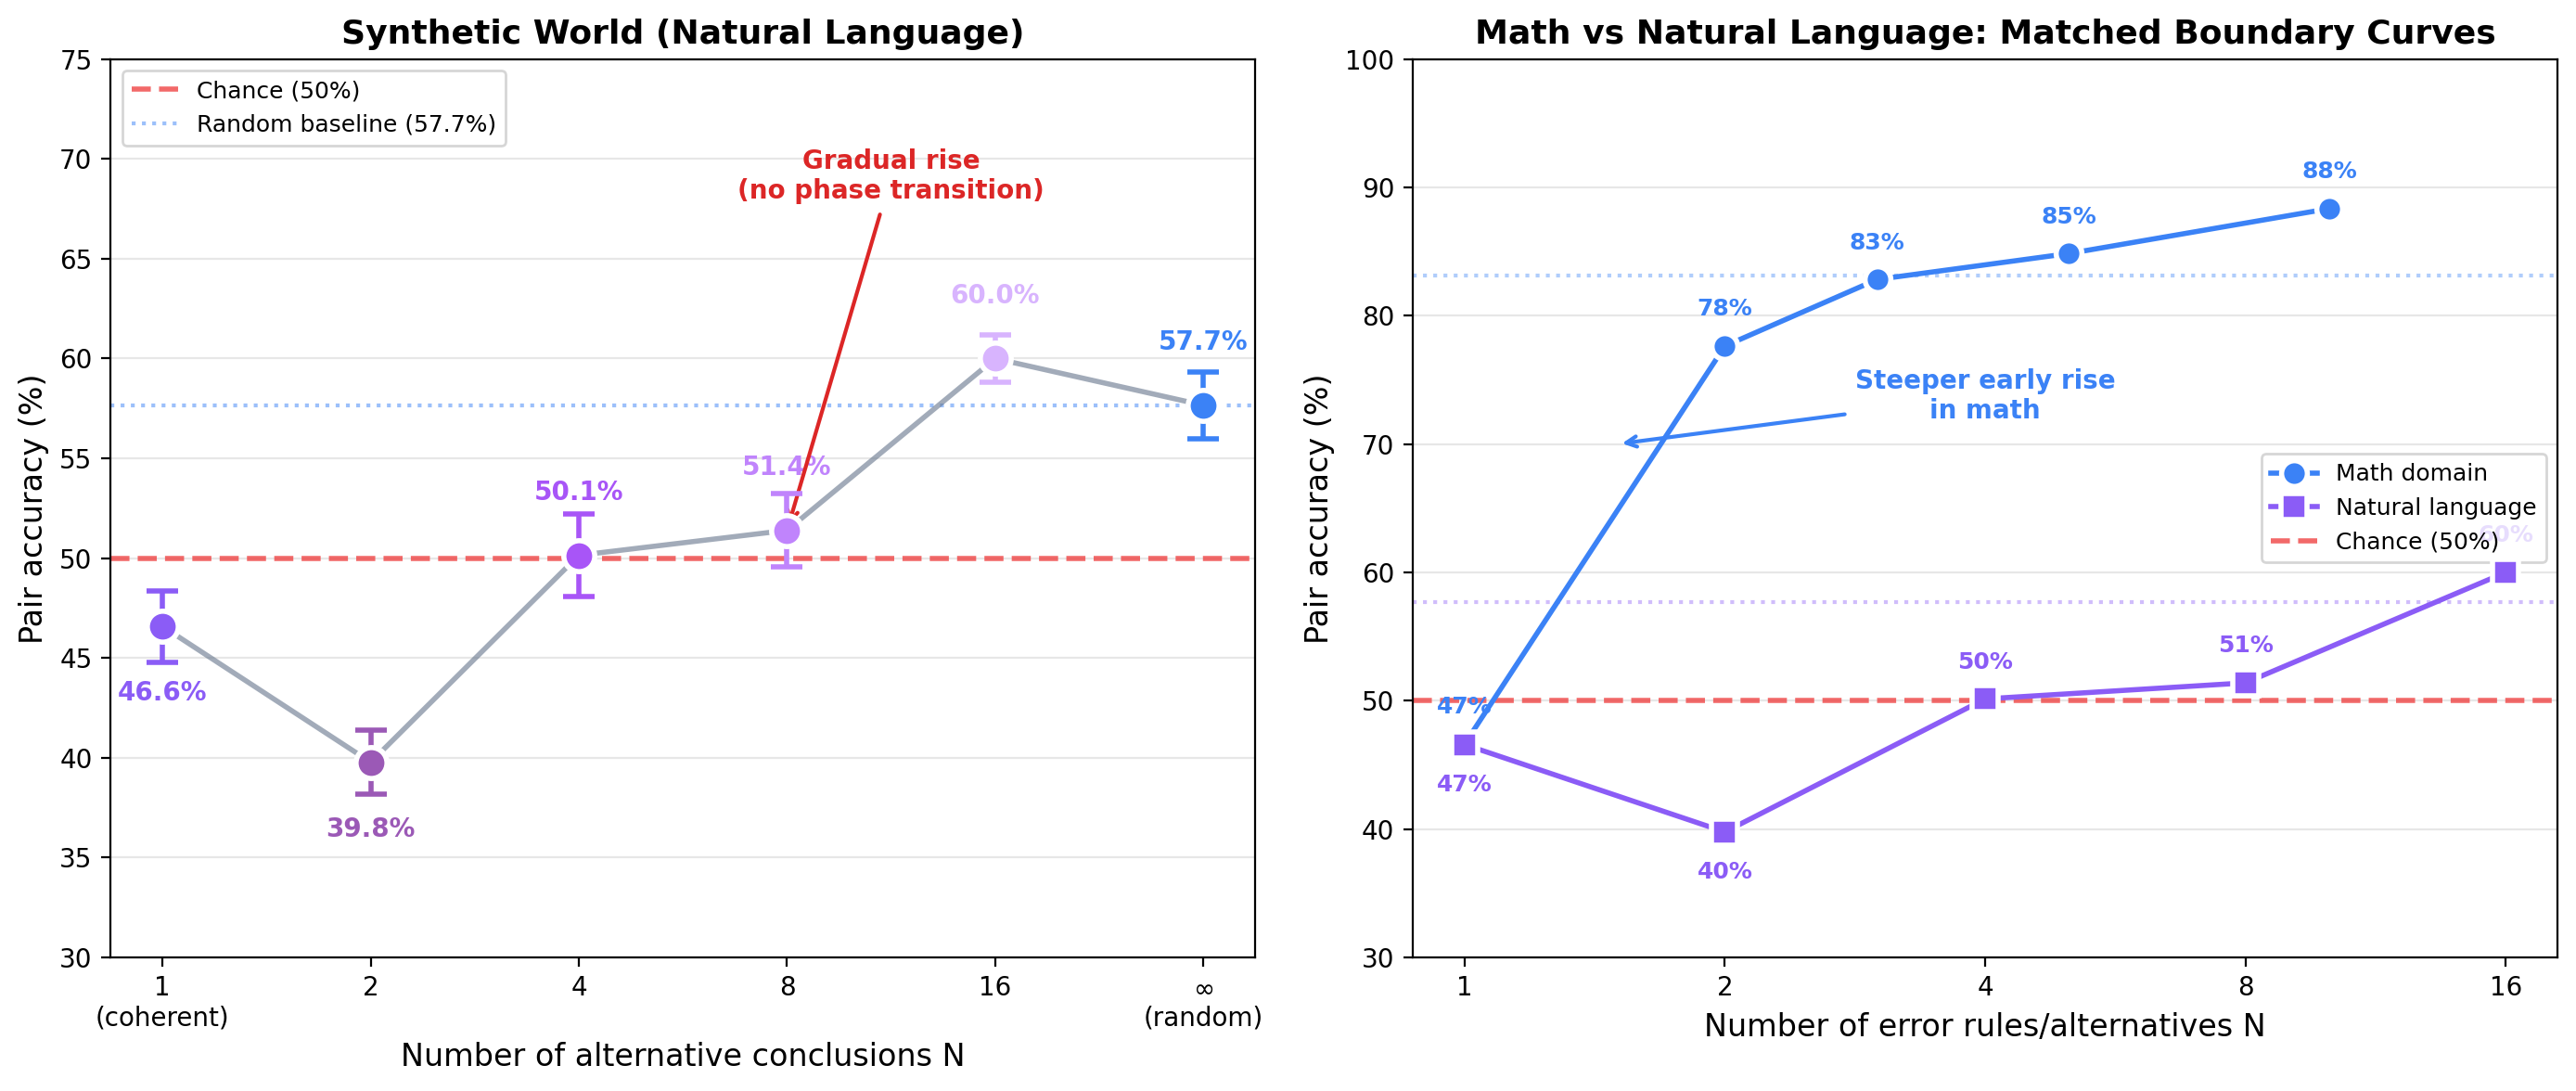
\includegraphics[keepaspectratio,alt={Figure B1}]{figure9_world_multialt.png}}
\caption{Figure B1}
\end{figure}

\emph{Figure B1. Multi-alternative errors in the synthetic world. Left:
pair accuracy as a function of the number of alternatives \texttt{N} --
gradual rise with no steep early jump. Right: comparison with the
revised matched math multi-rule curve, which rises much faster at low
\texttt{N} than the natural-language curve.}

Four observations:

\begin{enumerate}
\def\labelenumi{\arabic{enumi}.}
\item
  \textbf{No comparable early rise.} Unlike mathematics, where the
  matched multi-rule curve already reaches 77.6\% at \texttt{N=2}, the
  natural-language growth is gradual: 47\% -\textgreater{} 40\%
  -\textgreater{} 50\% -\textgreater{} 51\% -\textgreater{} 60\%. Even
  at \texttt{N=16}, accuracy is only 60\%, close to the result for fully
  random errors (57.7\%).
\item
  \textbf{N = 2 worsens the result.} With two alternatives, the model
  \emph{prefers} erroneous conclusions (39.8\% \textless{} 50\%), worse
  than a single coherent alternative (46.6\%). The likely reason: two
  alternatives create a distribution (each at \textasciitilde25\% of the
  corpus) that collectively competes with the correct conclusion (50\%)
  while remaining compressible.
\item
  \textbf{High accuracy vs random masks weak truth bias.} The same
  models trained on N = 2 show 97.3\% accuracy when compared against
  fully random errors. The model successfully learns all N alternative
  patterns but cannot distinguish them from truth -- both sets are
  equally well compressible.
\item
  \textbf{Natural language absorbs contradictions.} In formal
  mathematics, two contradictory rules (N = 2) immediately destroy
  compressibility: for arithmetic, \texttt{a\ +\ b\ =\ a\ +\ b\ +\ 1}
  and \texttt{a\ +\ b\ =\ a\ +\ b\ -\ 1} cannot be captured by a single
  function. In natural language, the phrases ``has thin scales'' and
  ``has dense armor plates'' are simply two textual patterns, each of
  which is easily memorized. The structure of text provides sufficient
  degrees of freedom to compress incompatible statements.
\end{enumerate}

This result has practical significance: \textbf{in domains with natural
language structure, compression pressure weakly distinguishes truth from
plausible misinformation}, even when the latter is internally
contradictory. This may help explain why LLMs readily memorize and
reproduce coherent misconceptions.

\subsubsection{B.3 Experiment 8: Cross-Domain
Falsification}\label{b.3-experiment-8-cross-domain-falsification}

One motivating finding of our experiments is that coherent falsehood can
become difficult to distinguish from truth under compression in isolated
domains: false derivative rules are tested only on derivative tasks. In
the real world, a false theory of derivatives conflicts with adjacent
domains (integration, tangent lines, numerical evaluation). We test
whether adding \emph{cross-domain} tasks -- correct tasks linking
derivatives with arithmetic -- can weaken the coherence of the false
rule.

Base corpus: coherent 50/50 (Section 4.2). We add correct cross-domain
tasks of five types: derivative evaluation at a point, antiderivative
check, tangent line equation, chain rule evaluation, and product rule
evaluation. All cross-domain tasks use the true differentiation rules.
We vary the proportion of cross-domain tasks: 0\%, 10\%, 25\%, 50\%.

\textbf{Table B3.} Cross-domain falsification (tiny, 3.5M, 4 seeds).
Paired evaluation on coherent paired test.

{\def\LTcaptype{none} % do not increment counter
\begin{longtable}[]{@{}
  >{\centering\arraybackslash}p{(\linewidth - 6\tabcolsep) * \real{0.3333}}
  >{\centering\arraybackslash}p{(\linewidth - 6\tabcolsep) * \real{0.2267}}
  >{\centering\arraybackslash}p{(\linewidth - 6\tabcolsep) * \real{0.2667}}
  >{\centering\arraybackslash}p{(\linewidth - 6\tabcolsep) * \real{0.1733}}@{}}
\toprule\noalign{}
\begin{minipage}[b]{\linewidth}\centering
Cross-domain proportion
\end{minipage} & \begin{minipage}[b]{\linewidth}\centering
Overall accuracy
\end{minipage} & \begin{minipage}[b]{\linewidth}\centering
Derivative accuracy
\end{minipage} & \begin{minipage}[b]{\linewidth}\centering
Other types
\end{minipage} \\
\midrule\noalign{}
\endhead
\bottomrule\noalign{}
\endlastfoot
0\% (baseline) & 47.0\% & 35.2\% & 51.1\% \\
10\% & 45.8\% & 39.4\% & 47.9\% \\
25\% & 50.6\% & \textbf{56.0\%} & 48.8\% \\
50\% & 47.1\% & 45.4\% & 47.6\% \\
\end{longtable}
}

\begin{figure}
\centering
\pandocbounded{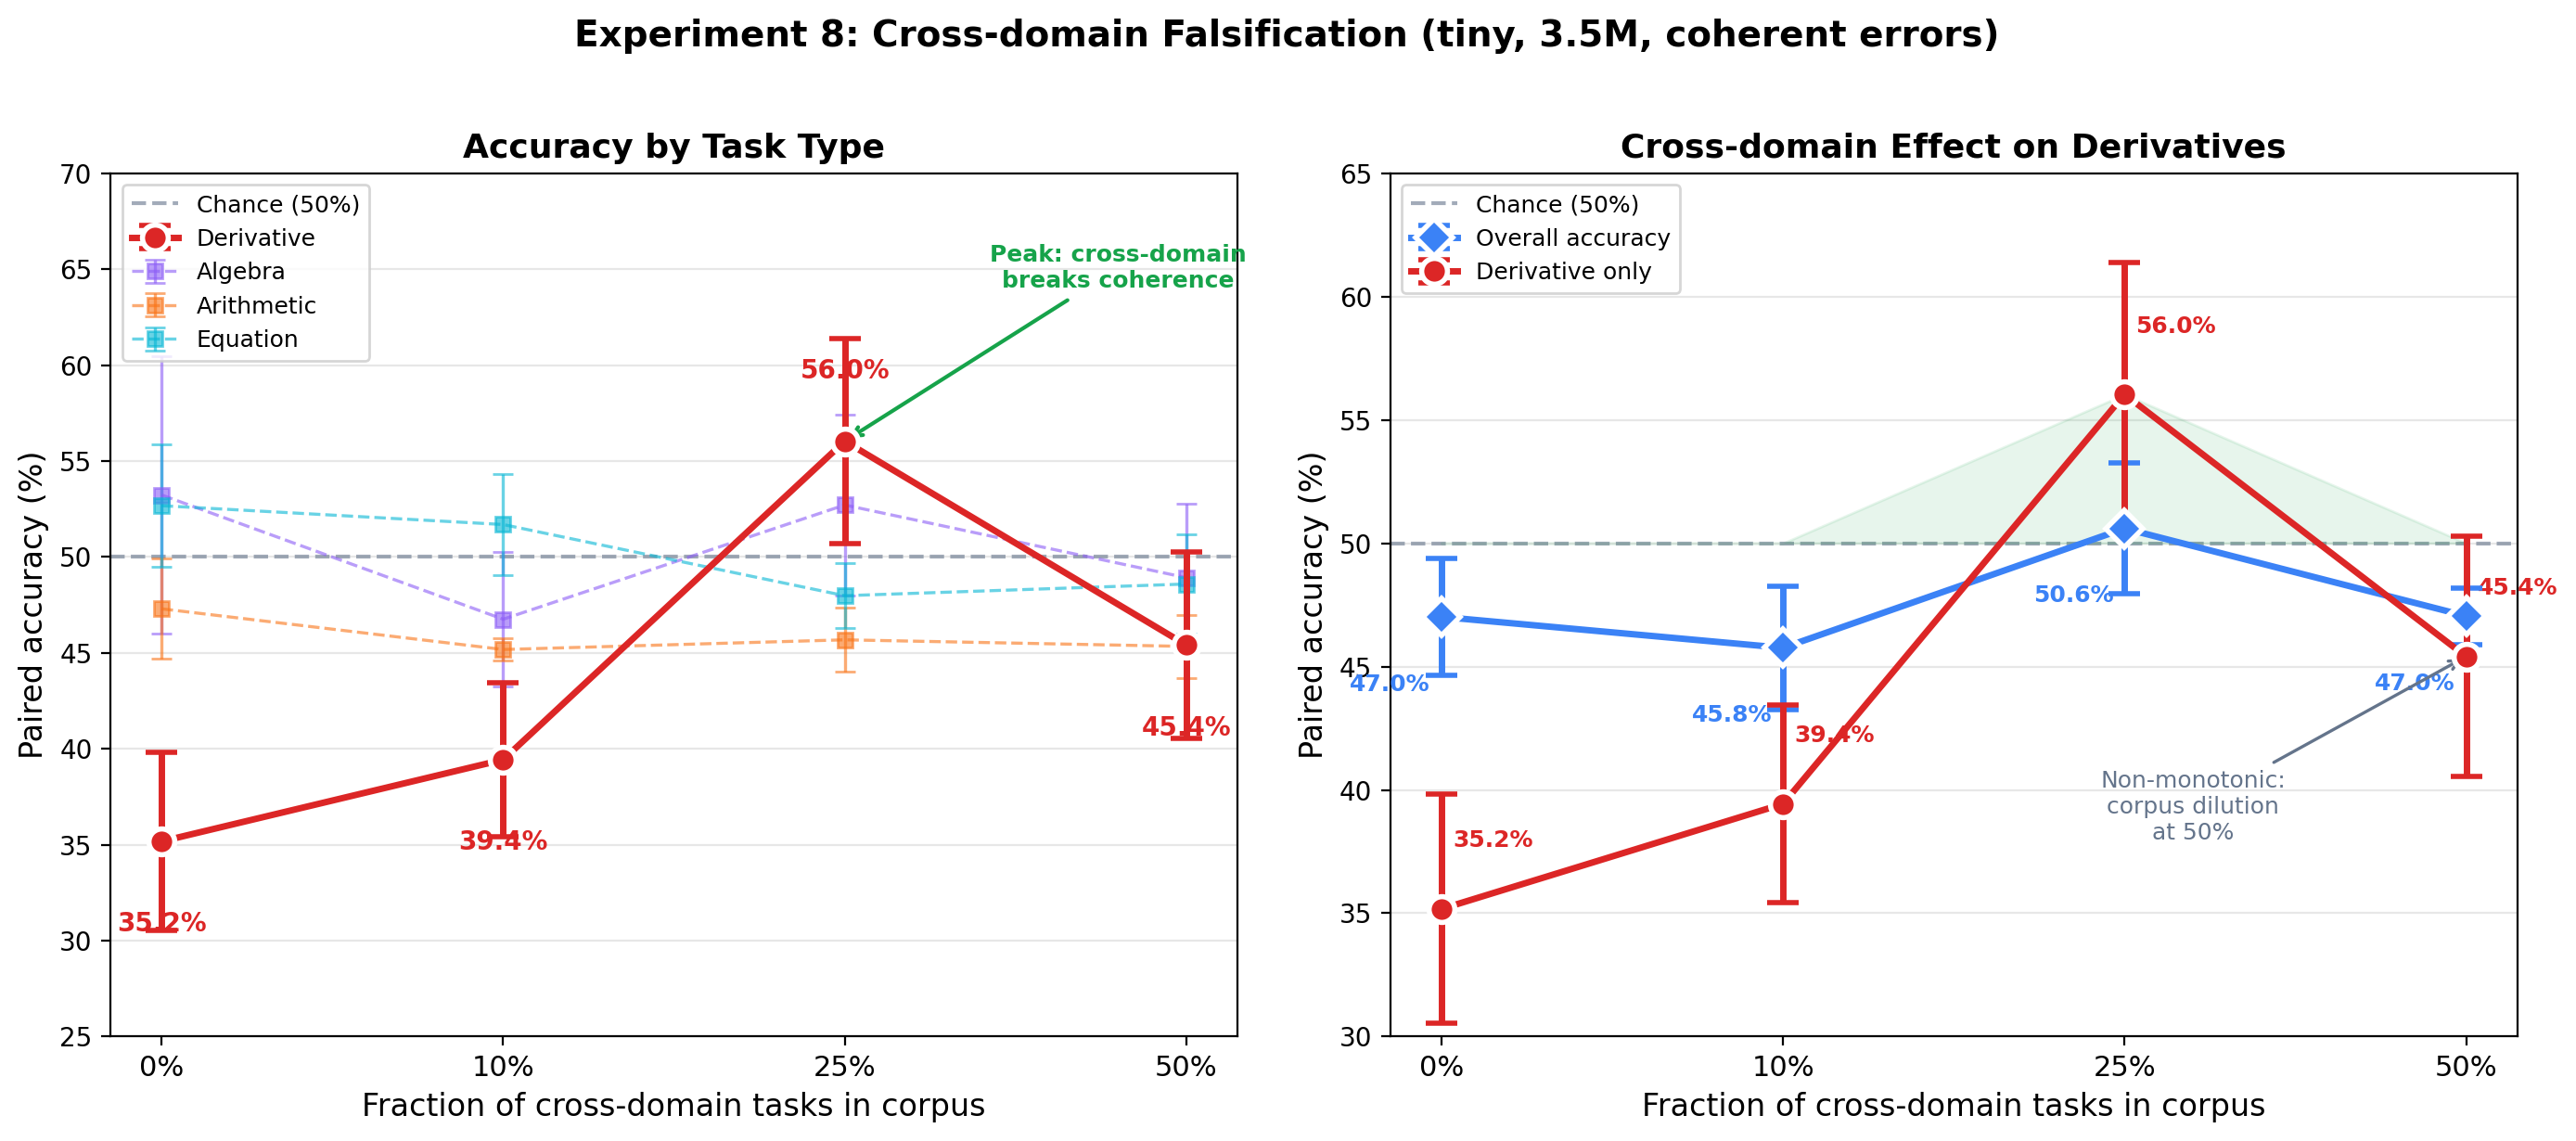
\includegraphics[keepaspectratio,alt={Figure B2}]{figure8_crossdomain.png}}
\caption{Figure B2}
\end{figure}

\emph{Figure B2. Cross-domain falsification. Left: accuracy by task type
--- only derivatives respond to cross-domain tasks. Right: non-monotonic
effect --- peak at 25\%, decline at 50\% due to corpus dilution.}

The result is directionally consistent with the hypothesis: accuracy on
\textbf{derivatives} increases from 35.2\% to 56.0\% at 25\%
cross-domain tasks, suggesting a shift toward correct derivatives in
that slice of the data. However, the effect is non-monotonic: at 50\%,
accuracy drops to 45.4\%, likely due to dilution of standard patterns.
Other task types (algebra, arithmetic, equations) remain at chance,
since the cross-domain tasks address only contradictions with
derivatives.

This experiment provides preliminary evidence that cross-domain data can
\emph{selectively} weaken the coherence of false rules. The effect is
still weak (derivative accuracy: 56\% vs 50\% chance), as expected for a
tiny model (3.5M). Scaling to larger models and expanding the set of
cross-domain tasks is a priority for future work.

\end{document}
